\documentclass[12pt]{article}
\RequirePackage{lineno}
\usepackage{fullpage}
\usepackage{breqn}
\usepackage{epsfig}
\usepackage{longtable}
\usepackage{fontenc}
\usepackage{graphicx}
\usepackage{times}
\usepackage{rotating}
\usepackage{psfrag}
\usepackage{graphics}
\usepackage{lscape}
\usepackage{xspace}
\usepackage{hyperref}
\usepackage{titlesec}

\setcounter{secnumdepth}{5}
\setcounter{tocdepth}{5}

\usepackage[firstpage]{draftwatermark}


\bibliographystyle{input/prsty}

\makeatletter
\renewcommand{\thefootnote}{\fnsymbol{footnote}}
\newcommand{\boldsymbol}[1]{\mbox{\boldmath $#1$}}
\makeatother

\def\totaldays{44.3~}
\def\productiondays{34~}
\def\overheaddays{10.3~}

\def\QMIN{0.2}
\def\QMAX{2.9}
\def\XMIN{0.30}
\def\XMAX{2.0}
\def\WMIN{1.8}
\def\WMAX{3.1}
\def\QMINT20{0.2}
\def\QMAXT20{1.8}
\def\Azz{$A_{zz}$}

\def\need{\textcolor{blue}{\textsuperscript{~[citation~needed]}}}

\def\SPOKES{1}
\def\CONTACT{2}

\def\PZ{50}     % Vector target polarization
\def\PZZ{30}
\def\PF{0.65}   % Packing Factor
\def\DF{0.285}   % Dilution Factor
\def\TARGET{ND$_3$ }
\def\CURRENT{80 } % nanoAmps
\def\LUMI{$1.2\times 10^{35}~\mathrm{cm}^{-2}\mathrm{s}^{-1}$}

\def\be{\begin{eqnarray*}}
\def\ee{\end{eqnarray*}}
\def\bn{\begin{eqnarray}}
\def\en{\end{eqnarray}}
\def\nn{\nonumber}

\def\ks{\vspace{1.1cm}\\}
\def\ls{\vspace{0.1cm}}

\def\n{\large}




%%%%%%%%%%%%%%%

\begin{document}
\SetWatermarkLightness{0.8}
\linenumbers
\pagestyle{empty}
 
\begin{center}
 \LARGE{
  Measurements of the Quasi-Elastic and Elastic Deuteron Tensor Asymmetries
%  Measurements of the Tensor Asymmetry $A_{zz}$ from $0.3<x<1.9$ and Elastic $T_{20}$
 }
- v 0.912
\end{center}
%
\hrule \vspace{.05cm}\hrule
%
\begin{center}
A Proposal to Jefferson Lab PAC 43

(Update to LOI12-14-002)

%\vspace{1.5cm}
\vspace{15px}

\setcounter{footnote}{\SPOKES}
%
{~~E. Long,\setcounter{footnote}{\SPOKES}
\setcounter{footnote}{\SPOKES}\footnotemark \footnotetext{Spokesperson}
\setcounter{footnote}{\CONTACT}\footnotemark\footnotetext{Contact: \href{mailto:ellie@jlab.org}{ellie@jlab.org}}
~~K. Slifer,\setcounter{footnote}{\SPOKES}\footnotemark
~~P. Solvignon,\setcounter{footnote}{\SPOKES}\footnotemark
~~T. Badman,
~~S. Li,
~~K. McCarty,
~~C. Meditz,
~~M. O'Meara,
~~R. Paremuzyan,
~~S. Santiesteban,
~~B. Yale,
~~R. Zielinski
}\\
\ls
{\normalsize\it{University of New Hampshire, Durham, NH 03861}}

\vspace{10px}

{~~D. Day,\setcounter{footnote}{\SPOKES}\footnotemark
~~D. Keller,\setcounter{footnote}{\SPOKES}\footnotemark
~~D. Crabb,
~~S. Liuti,
~~O. A. Rondon,
~~V. Sulkosky}\\
\ls
{\normalsize\it{University of Virginia, Charlottesville, VA 22903}}

\vspace{10px}

{~~D. Higinbotham\setcounter{footnote}{\SPOKES}\footnotemark,
~~A. Camsonne,
~~S. Covrig Dusa,
~~D. Gaskell,
~~C. Keith,
~~P. Nadel-Turonski}\\
\ls
{\normalsize\it{Thomas Jefferson National Accelerator Facility, Newport News, VA 23606}}

\vspace{10px}

{~~Z. Ye}\\
\ls
{\normalsize\it{Duke University, Durham, NC 27708}}

\vspace{10px}

{~~N. Kalantarians}\\
\ls
{\normalsize\it{Hampton University, Hampton, VA 23668}}

\vspace{10px}

{~~A. Ahmidouch,~~S. Danagoulian}\\
\ls
{\normalsize\it{North Carolina A\&T State University, Greensboro, NC 27411}}

\vspace{10px}

{~~M. Sargsian,
~~P. Markowitz}\\
\ls
{\normalsize\it{Florida International University, Miami, FL 33199}}

\vspace{10px}

{~~W. Cosyn}\\
\ls
{\normalsize\it{Ghent University, 9000 Ghent, Belgium}}

\vspace{10px}

{~~M. Strikman}\\
\ls
{\normalsize\it{Pennsylvania State University, University Park, PA 16802}}

\vspace{10px}

{~~G. A. Miller}\\
\ls
{\normalsize\it{University of Washington, Seattle, WA 98195}}

\vspace{10px}

{~~J. Beri\v{c}i\v{c}, 
~~T. Brecelj, 
~~S. \v{S}irca, 
~~S. \v{S}tajner} \\
\ls
{\normalsize\it{Jo\v{z}ef Stefan Institute and University of Ljubljana, Slovenia}}

\vspace{10px}

{~~K. J. Park}\\
\ls
{\normalsize\it{Old Dominion University, Norfolk, VA 23529}}

\vspace{10px}

{~~M. Elaasar}\\
\ls
{\normalsize\it{Southern University and New Orleans, New Orleans, LA 70126}}

\vspace{10px}

{~~W. van Oers}\\
\ls
{\normalsize\it{University of Manitoba, Winnipeg, MB, Canada}}

\vspace{10px}

{~~B. Bertozzi,
~~S. Gilad}\\
\ls
{\normalsize\it{Massachusetts institute of Technology, Cambridge, MA 02139}}

\vspace{10px}

{~~K. Adhikari}\\
\ls
{\normalsize\it{Mississippi State University, Mississippi State, MS 39762}}
\ks

%



\end{center}

%\footnotetext{Co-spokesperson}
%\footnotetext{Contact person}

\setcounter{footnote}{0}


\newpage

\begin{abstract}
  We propose the first measurement of the tensor asymmetry $A_{zz}$ in the quasi-elastic region through the tensor polarized D($e,e'$)X channel; an asymmetry that is sensitive to the nucleon-nucleon potential.  Previous measurements of $A_{zz}$ have been used to extract $b_1$ in the DIS region and $T_{20}$ in the elastic region. In the quasi-elastic region, $A_{zz}$ data will be used to compare light cone calculations with variation nucleon-nucleon calculations, and is an important quantity to determine for understanding tensor effects, such as the dominance of $pn$ correlations in nuclei.


In the quasi-elastic region, $A_{zz}$ was first calculated in 1988 by Frankfurt and Strikman, using the Hamada-Johnstone and Reid soft-core wave functions~\cite{Frankfurt:1988nt}. Recent calculations by
M. Sargsian revisit $A_{zz}$ in the $x > 1$ range using virtual-nucleon and light-cone methods, which differ by up to a factor of two~\cite{MISAK} and can be discriminated experimentally at the $3-6\sigma$ level. This potential measurement has stirred the interest of a number of theorists, and will be proposed in full as calculations solidify.

We propose an experimental determination of $A_{zz}$  utilizing the same equipment as the E13-12-011 $b_1$ experiment.  Three different $Q^2$ values will be measured over the course of \productiondays days, with \overheaddays additional days of overhead. The measurements are less sensitive to systematic uncertainties than E13-12-011, so this experiment would be utilized in parallel to better understand the in-beam conditions and time-dependent systematic effects of a tensor polarized target for the $b_1$ experiment.




%We propose the first measurement of the tensor asymmetry $A_{zz}$ in the quasi-elastic region through the $\stackrel{\leftrightarrow}{\mathrm{D}}$($e,e'$)X channel to determine information on the tensor portion of the deuteron wavefunction. Previous measurements of $A_{zz}$ have been used to extract $b_1$ in the DIS region and $T_{20}$ in the elastic region. In the quasi-elastic region,  $A_{zz}$ can be used to extract the ratio of the S and D-states in the deuteron wave function. This ratio is currently not well constrained experimentally and is an important quantity to determine for understanding tensor effects, such as NN short range correlations, and is most clearly manifested in the scattering off the polarized deuteron due to a strong dependence of the S/D ratio on the nucleon momentum.

%In the quasi-elastic region, $A_{zz}$ was first calculated in 1988 by Frankfurt and Strikman, using the Hamada-Johnstone and Reid soft-core wave functions \cite{Frankfurt:1988nt}. Recent calculations by {M.~Sargsian} revisit $A_{zz}$ in the $x>1$ range using virtual-nucleon and light-cone methods, which differ by up to a factor of two \cite{MISAK} and can be discriminated experimentally at the $3-6 \sigma$ level.

%An experimental determination of $A_{zz}$ could be performed utilizing identical equipment identical as the E13-12-011 $b_1$ experiment at three different $Q^2$ values over the course of \productiondays days, with \overheaddays additional days of overhead. The measurements are less sensitive to systematic uncertainties than E13-12-011, such that this experiment could additionally be utilized to understand the in-beam conditions and time-dependent systematic effects of a tensor polarized target.

\end{abstract}

\newpage

%\section*{Foreword}

%This proposal is an update to PR12-11-110 which was submitted to PAC38.  For convenience, we reproduce the PAC report on the next page.   We provide here an overview of the actions we've taken to address the PAC concerns. Full details are available in the main text.

As suggested by PAC38, we have modified our experimental technique to measure the tensor asymmetry instead of the cross section difference.  This takes the simplified form of the ratio of tensor polarized to unpolarized cross-sections shown in Eq.~\ref{3}.   While this cancels the largest first order effects\footnote{For example, the target magnetic field will be oriented along the beamline during both polarized and unpolarized data taking, which greatly reduces the sensitivity to changes in acceptance in the two configurations.}, special care will be needed to control the sensitivity of the integrated counts in each state to time dependent drifts in detector response, charge measurement and luminosity. 

We have assumed a tensor polarization (P$_{zz}$=\PZZ\%) which is larger than the previous proposal. This assumption is based on the documentation of tensor polarized targets previously discussed in publications, and is supported by the experience of the collaboration's polarized target groups.   This will require incremental development of existing DNP techniques.  We acknowledge that less established methods, such as the `hole-burning' technique recommended by the PAC, hold very good potential to produce significantly higher tensor polarization, but this will require significant R\&D.  We have initiated this process, although from a practical perspective, the funding for this development will likely remain limited until an approved experiment demonstrates the need for these novel tensor polarized targets. 

The $x_B$-coverage has been expanded, although we note that a significantly non-zero value of $b_1$ at any $x_B$ would unambiguously confirm its non-conventional behavior.  Finally, we have engaged several theorists for calculations and to confirm that our interpretation of the relationship between the measured asymmetry and the tensor structure function $b_1$ is valid.



\newpage
\subsection*{PAC38 Report}
{
\noindent
{\bf PR12-11-110} ``The Deuteron Tensor Structure Function b1''

\vspace{0.1cm}
\noindent
{\bf Motivation}: This proposal, a follow-up of LOI-11-003 submitted to PAC37, is dedicated to the measurement of the deuteron tensor structure function $b_1$ by measuring deep inelastic scattering from a tensor polarized deuterium target. All available models predict a small or vanishing value of $b_1$ at low x, however the first pioneering measurement of $b_1$ at HERMES revealed a crossover to an anomalously large negative value, albeit with a relatively large experimental uncertainty. This justifies the intention to make a precise measurement: confirmation that $b_1$ is relatively large may then require an explanation based on more exotic models for the deuteron, such as hidden color due to a 6-quark configuration.

%\vspace{1cm}
\noindent
{\bf Measurement and Feasibility}: The collaboration proposes to carry out this experiment in Hall C, using the polarized UVa/JLab ND$_3$ target, the HMS/SHMS spectrometers and an unpolarized 115 nA electron beam. The tensor structure function $b_1$ is derived from the measurement of the difference between the transversely and longitudinally tensor polarized cross-sections, which is directly proportional to $b_1$ itself. From the measured value of $b_1$ the tensor asymmetry $A_{zz}$ can be calculated, provided the structure function $F_1$ is known. The collaboration proposes to perform the measurement in 28 days of data taking at 11 GeV at the two x values of 0.3 and 0.5, which cover the range in which the HERMES data display the crossover of $b_1$ to large negative values.



%\vspace{1cm}
\noindent
{\bf Issues}: Despite the interesting physics case presented, the PAC has identified several issues with this proposal.
\begin{enumerate}
\item One obvious problem is the theoretical interpretation of the results of this kind of experiments. Following the recommendation of PAC37 the collaboration has partially addressed this question by expanding the discussion of the expected behavior of $b_1(x)$ in various theoretical models. However to draw significant conclusions from this measurement, also given the limited kinematical coverage (see below) chosen, would require further work.
\item The chosen x range, although overlapping with the region in which the HERMES results were obtained, does not seem sufficient to determine $b_1(x)$ in such a way as to unambiguously establish its conventional or exotic behavior. The PAC encourages the collaboration to explore the possibility to carry out the measurement using a large acceptance spectrometer covering a wider x range.
\item The PAC has concerns about the proposed experimental method using the cross section difference between the transversely and longitudinally tensor polarized target configurations. Given a 5-tesla field for this type of target, the effect on the acceptance due to the target field for these configurations can be quite different, and such systematic uncertainties due to the acceptance and other effects may well be larger than the effect that the proponents are trying to measure.
\item The proponents should pursue the tensor asymmetry measurement technique. Currently, the proposed target has a rather low tensor polarization ($\sim$10\%). It is crucial and important to pursue more vigorously techniques such as the RF ``hole’’ burning technique to improve the tensor polarization of the target.
%}
\end{enumerate}
}




\clearpage


\tableofcontents


\pagestyle{plain}

\clearpage

%\section{Quotes (To be removed)}
%\input{input/0_quotes.tex}

\section{$A_{zz}$ Motivation}

%For decades~\cite{PhysRev.81.165}, it has been known that the nucleon-nucleon potential has a short-range repulsive core, which is responsible for the stability of strongly interacting matter. However, a description of the repulsive core remains largely unconstrained and our understanding of QCD dynamics at short distances ($\leq 0.5\mathrm{~fm}$) largely incomplete~\cite{Sargsian:2014bwa}. 

The deuteron is the simplest composite nuclear system, and in many ways it is as important to understanding bound states in QCD as the hydrogen atom was to understanding bound systems in QED.  Our experimental and theoretical understanding of the deuteron remains unsatisfying, which we will address by measuring the tensor asymmetry $A_{zz}$ for the first time in a kinematic region where theoretical understanding of the deuteron is weak.

Due to their small size and simple structure, tensor polarized deuterons are ideal for studying nucleon-nucleon interactions. Tensor polarization enhances the D-state contribution, which compresses the deuteron~\cite{Forest:1996kp}, 
%in a toroid as shown in Fig.~\ref{fig:dpol-shape}, 
making the system more sensitive to short-range QCD effects. Understanding the nucleon-nucleon potential of the deuteron is essential for understanding short-range correlations as they are largely dependent on the tensor force~\cite{Arrington:2011xs}. We can resolve the short-range structure of nuclei on the level of nucleon and hadronic constituents by utilizing processes that transfer to the nucleon constituents both energy and momentum larger than the scale of the NN short-range correlations, particularly at $Q^2>1~(\mathrm{GeV}/c)^2$.


By taking a ratio of cross sections from electron scattering from tensor-polarized and unpolarized deuterons, 
\begin{equation}
A_{zz}=\frac{2}{fP_{zz}}\left(\frac{\sigma_p}{\sigma_u}-1\right),
\end{equation}
the S and D-wave states can be disentangled, leading to a fuller understanding of the repulsive nucleon core. A measurement of $A_{zz}$ is sensitive to the ratio $\frac{D^2-SD}{S^2+D^2}$ and it's evolution with increasing minimal momentum of the struck nucleon. Originally calculated by L.~Frankfurt and M.~Strikman~\cite{Frankfurt:1988nt}, this has recently been revisited by M.~Sargsian and M.~Strikman, who calculated $A_{zz}$ in this region using light cone and virtual nucleon approaches with multiple NN potentials~\cite{Sargsian:2014fla}. The calculations vary by up to a factor of 2, and can be experimentally determined at the $3-6\sigma$ level as discussed in this proposal. In this same region, effects from final state interactions have been calculated and are expected to have a significant effect at large $x$~\cite{cosyn-convo}.


For the lower $Q^2$ region, W. Van Orden has calculations in progress using different nucleon-nucleon potentials, as well as different prescriptions for handling the reaction mechanisms in tensor polarization observables in the low $Q^2$ region~\cite{vanorden-convo}. Although it is difficult to disentangle reaction mechanisms from NN potentials using cross section measurements, previous low $Q^2$ results have indicated that asymmetries are far less sensitive to the reaction mechanisms~\cite{Passchier:2001uc}. Similar calculations have recently been finalized for the D($e,e'p)n$ at high $Q^2$, high $p_m$ experiment~\cite{Ford:2014yua}. 

Additionally, measuring $A_{zz}$ in the quasi-elastic region will fill a gap in measurements performed on deuterium scattering. It is directly proportional to the elastic deuteron tensor analyzing powers by $A_{zz} = \sqrt{2} \left[ d_{20} T_{20} + d_{21} T_{21} + d_{22} T_{22}\right]$. Due to the large acceptance of the SHMS spectrometer, we will be taking data in the $x = 2$ elastic range as well, allowing us to measure $T_{20}$ at a large range in $Q^2$ (as contributions from $T_{21}$ and $T_{22}$ are small). In the deep inelastic region, $A_{zz}$ will soon be measured to extract the tensor structure function $b_1$ by the relation $A_{zz} \propto \frac{b_1}{F_1^D}$. Not only will measuring $A_{zz}$ in the quasi-elastic region provide information necessary for understanding the fundamental properties of the deuteron, but it will be the first experiment to bridge a gap in measurements of electron scattering from tensor-polarized deuterons. We emphasize that this measurement is pushing the limits of understanding the deuteron by going to kinematics where no no current measurements exist and where current theoretical understanding remains unsatisfying.





\subsection{Probing the Deuteron Wavefunction}

It was suggested for some time~\cite{Frankfurt:1981mk} that to resolve the microscopic structure of nuclei one needs to study scattering at sufficiently large momentum transfer and large relative momenta of the produced nucleons. This logic was confirmed~\cite{Arrington:2011xs} by a series of experiments at SLAC~\cite{Frankfurt:1993sp} and JLab~\cite{Arrington:1998ps,Fomin:2011ng} that directly observed short-range correlations (SRC) in a series of nuclei, and established a similar effect of SRC in the deuteron and in heavier nuclei with $pn$ correlations giving the dominant contribution.  Hence, the deuteron serves as a ``hydrogen atom" for the studies of the microscopic short-range structure of the nuclei since it is the simplest nuclei that follows SRC scaling.

To achieve further progress, it is necessary to improve our knowledge of the deuteron wave function at high momenta, and to separate the S and D contributions to the high momentum component of the deuteron. The dominance of the D-wave at a large range of the nucleon momenta is expected in a range of the theoretical models, as demonstrated in Fig.~\ref{sd-wf}, but experimentally it was probed in a rather indirect way via measurement of $T_{20}$ for the deuteron form factor~\cite{Garcon:2001sz}. Still, the knowledge of S/D ratio for large momenta is rather poor. Indeed, all wavefunctions are constrained by low energy data to reproduce the S/D ratio at small momenta while the overall probability of the D-wave in the deuteron differs by a factor up to 1.5, leading to a large difference of the S/D ratio at large momenta.

The S and D-states are related to the tensor asymmetry $A_{zz}$ by~\cite{Frankfurt:1988nt}
\begin{equation}
	A_{zz} \propto \frac{\frac{1}{2}w^2(k)-u(k)w(k)\sqrt{2}}{u^2(k)+w^2(k)},
\end{equation}
where $u(k)$ is the S-state wave function and $w(k)$ is the D-state wave function. Additionally, measuring $A_{zz}$ at lower $Q^2$ will map out the transition from hadronic to partonic degrees of freedom.

\begin{figure}
\begin{center}
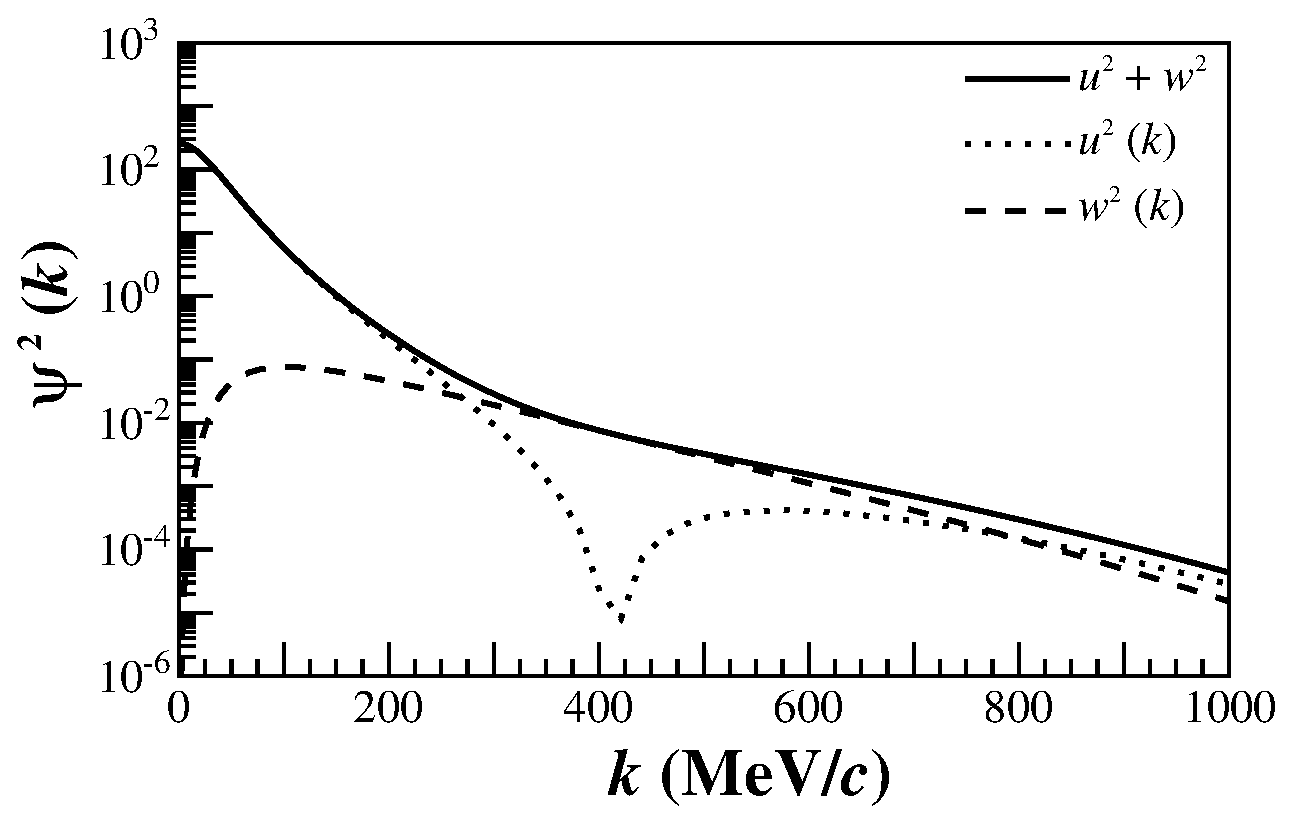
\includegraphics[width=0.55\textwidth]{figs/sd_wf_av18.eps}
\caption{\label{sd-wf} The AV18~\cite{PhysRevC.84.034003} deuteron wave-function, showing the dominance of the D-state (dashed) in comparison to the S-state (dotted) in the full wavefunction (solid) at high momentum ($k>300\mathrm{~Mev}/c$).}
\end{center}
\end{figure}

Ratios of inclusive cross sections at $x>1$ has demonstrated an early onset of the scaling of the ratios when plotted as a function of the light-cone fraction of the struck nucleon momentum.  As a result, the ratios provide a direct measurement of the ratio of the high momentum components in nuclei.  Similarly, one can expect that in the case of scattering from the polarized deuteron we expect the early scaling for the asymmetry when plotted as a function of the minimal struck nucleon momentum or the light cone fraction in the A($e,e'$) case.
It was observed at JLab that the scaling of the ratios set in starting at $Q^2 \sim 1 \mathrm{~GeV}^2$~\cite{Arrington:1998ps} so covering the range of $Q^2$ up to 2~GeV$^2$ will be sufficient to  measure the S/D ratios in an interesting momentum range. 





%For decades~\cite{PhysRev.81.165}, it has been known that the nucleon-nucleon potential has a short-range repulsive core, which is responsible for the stability of strongly interacting matter. However, a description of the repulsive core remains largely unconstrained and our understanding of QCD dynamics at short distances ($\leq 0.5\mathrm{~fm}$) largely incomplete~\cite{Sargsian:2014bwa}. 


It is worth noting here that in addition to comparing predictions for the different wave functions, one expects to be able to distinguish between non-relativistic and light cone quantum mechanic models.  The principal difference between the models is the relation between the spectator momentum and momentum in the wave function. In the nonrelativistic model they coincide, while in the light cone model the relation is non-linear starting at $k \sim 250 \mathrm{~MeV}/c$. This difference is most clearly manifested in the scattering from the polarized deuteron due to a strong dependence of the S/D ratio on the nucleon momentum.



\subsection{Study of the Relativistic NN Bound System}

One of the important issues in studying nuclear structure  at short distances is the 
relativistic description of the bound system.  This is an important issue also in 
understanding the QCD medium effect with recent studies indicating that  parton distribution 
modifications  in nuclei are proportional to the high momentum component of nuclear wave function~\cite{Weinstein:2010rt}.

The deuteron is the simplest bound system and naturally any self-consistent attempt  to understand the 
relativistic effects in the bound nuclear systems  should start with the deuteron. 
The issue of the relativistic description of the deuteron has a long history with extensive research that started in the late 1970's~\cite{Gross:1982nz,Buck:1979ff,Frankfurt:1977vc,Frankfurt:1981mk}.

Experimental studies of relativistic effects in the deuteron  up to now include the large $Q^2$ elastic 
$ed$ scattering~\cite{Alexa:1998fe}, however  
due to complexities  in the reaction mechanism~\cite{VanOrden:1995eg} the relativistic effects were 
difficult to isolate.

Inclusive D$(e,e')$X experiments from tensor-polarized deuterons at  $Q^2>1$~GeV$^2$ and in the $x>1$ region gives 
a new possibility to probe the relativistic structure of the deuteron.  In this case the use of the tensor polarized
deuteron allows us to prepare the nucleus in the most compact state in which, due to the absence of the 
pure S-wave contribution, the system in average is sensitive to the higher nucleon momenta in the deuteron.
At large $Q^2>1$ GeV$^2$ kinematics, the probed longitudinal momenta of the bound nucleon is given by $p_z \approx m_N(1-x)$, 
or the light cone momentum fraction $\alpha \ge x$. Because of these kinematic conditions and the enhancement of the 
D-wave contribution from tensor polarization, a measurable relativistic effects is expected already at $x\approx 1.2$.  Such an early onset of the relativistic effects indicates that they can be separated from the choice of NN potentials, which dominate at $x>1.4$. 

%The biggest advantage is that one expects less uncertainty at $x<1.3$ due to the choice of the NN potential and reaction dynamics due to relatively small values of the bound nucleon momenta involved ($\ge 200~\mathrm{MeV}/c$).

The sensitivity to relativistic effects is estimated using the theoretical calculations based on two 
very different approaches.   The first approach treats the  virtuality of the bound nucleon within a
description of the deuteron in the lab frame by treating the interacting nucleon as being 
virtual (virtual nucleon, or VN approximation). This is accomplished by taking the residue over the energy of the spectator nucleon.
In this case, the deuteron wave function satisfies the covariant equation of the two-nucleon bound system 
with one spectator being on energy shell~\cite{Sargsian:2009hf,Gross:2010qm}.

Another approach is based on the observation that high energy processes
evolve along the light-cone (LC).  Therefore, it is natural to describe the 
reaction within the light-cone non-covariant framework \cite{Frankfurt:1981mk}. 
Negative energy states do not enter in this case, though one has to take into 
account so called instantaneous interactions.
In the approximation when non-nucleonic degrees of freedom 
%in the deuteron wave function 
can be neglected, assuming rotational invariance of the LC deuteron wave function around its quantization axis, the relativistic wave function can be related to the nonrelativistic wave function through the introduction of LC $pn$ relative momentum~\cite{Frankfurt:1981mk, Miller:2009fc},

%one can relate the light-cone wave functions to those calculated in the lab frame by introducing the LC $pn$ relative three momentum,
\begin{equation}
k=\sqrt{{m^2+p_t^2\over \alpha(2-\alpha)} - m^2}.
\end{equation}

In Fig.~\ref{fig:misak}, the prediction for VN~\cite{Sargsian:2009hf} and LC~\cite{Frankfurt:1993sp} approximations are given 
for the highest $Q^2$ kinematics proposed. As was previously mentioned, a measurable 
difference is predicted to be observable already at $x\ge 1.2$.
% where one expects little uncertainty due to the choice of the wave function.  
 
 

\begin{figure}
\begin{center}
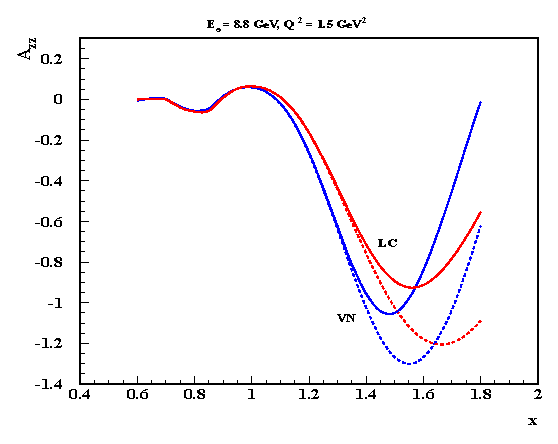
\includegraphics[width=0.49\textwidth]{figs/mark_misak_azz.eps}  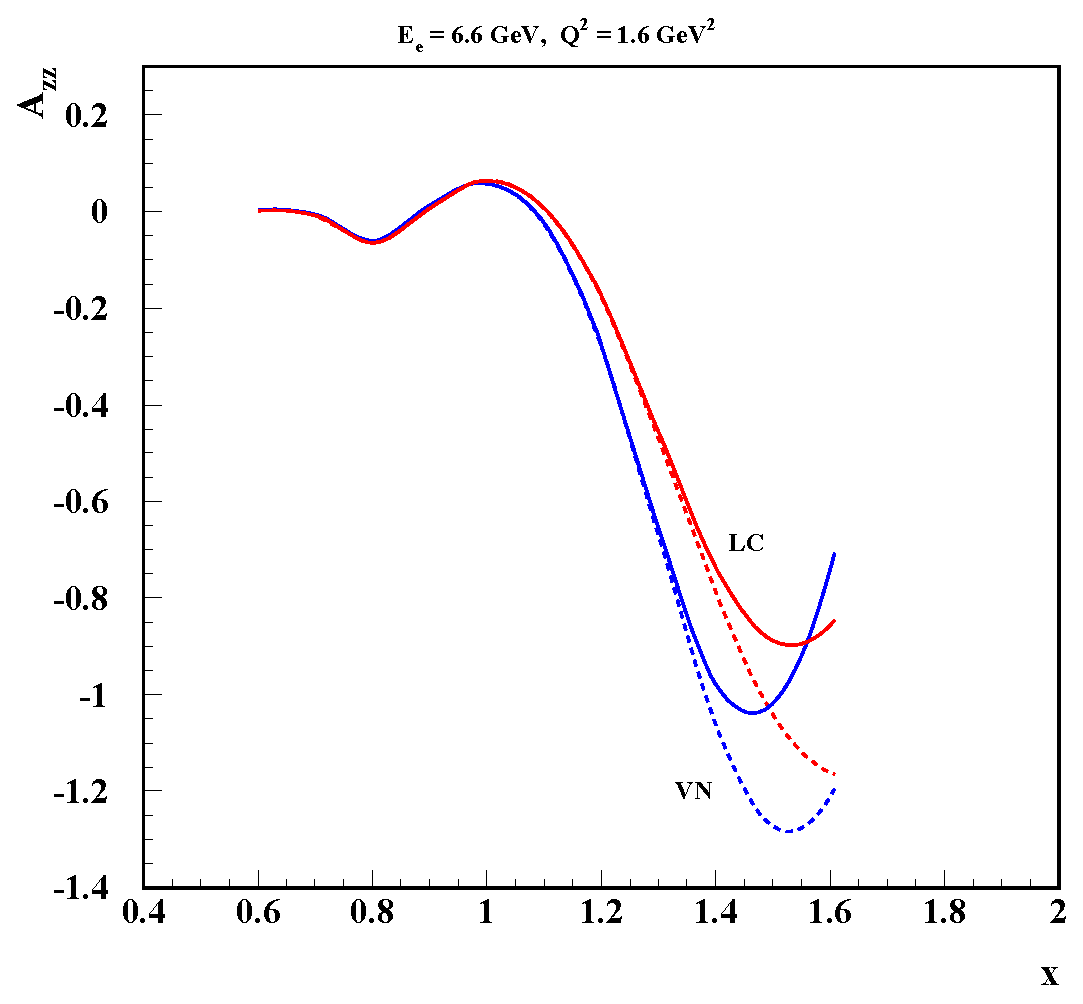
\includegraphics[width=0.49\textwidth]{figs/h2_ratio_t20_sigma.eps}
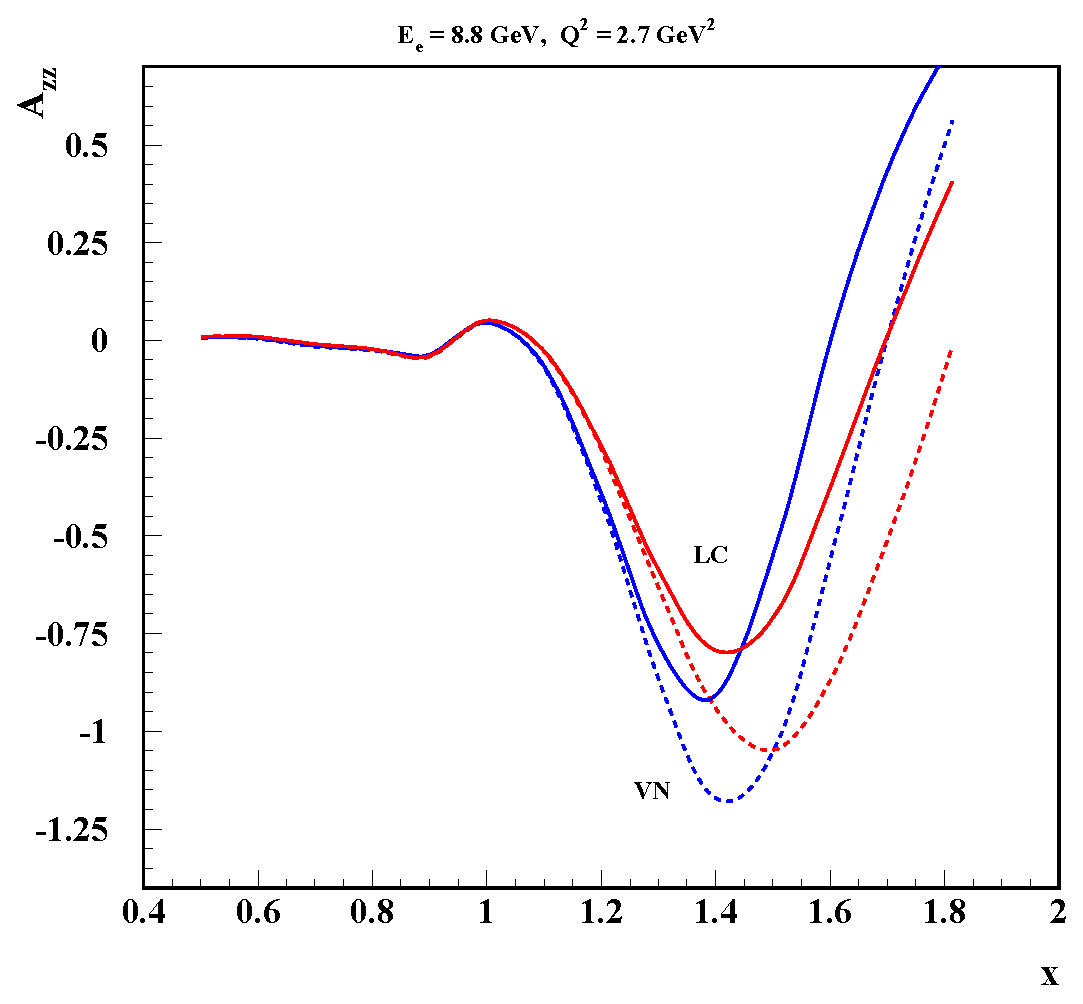
\includegraphics[width=0.49\textwidth]{figs/h1_ratio_t20_sigma.eps}
\caption{\label{fig:misak} The $A_{zz}$ observable calculated at $Q^2=1.5$, 1.8, and $2.9~(\mathrm{GeV}/c)^2$ using the light-cone (red) and virtual nucleon (blue) models with NN potential inputs of AV18 (solid) and CDBonn (dotted). Calculations provided by M. Sargsian and M. Strikman~\cite{Sargsian:2014fla,misak-convo}.}
\end{center}
\end{figure}




\subsection{Final State Interactions}

In order to accurately determine the nucleonic components of the deuteron's wave function, it is vital that final state interactions (FSI) are understood. As demonstrated below, FSI can introduce a significant component to $A_{zz}$, particularly in the large $x>1.2$ region. Including these effects is necessary for further constraining our theoretical understanding of the deuteron through $A_{zz}$.

The effects of FSI on $A_{zz}$ have recently been modeled by W. Cosyn in the deep-inelastic region~\cite{Cosyn:2014sqa} and in the quasi-elastic region discussed in this proposal~\cite{cosyn-convo}, which is an on-going area of research. Results are shown in Fig.~\ref{fig:fsi-kin1}-\ref{fig:fsi-kin2}. The calculations use the virtual nucleon (VN) approximation to compute inclusive observables in electron-induced scattering off the deuteron including the 
effect of final-state interactions. Amplitudes and observables are computed in an unfactorized manner.   

Current calculations include on-shell and off-shell contributions to the FSI amplitudes, but the off-shell contribution is calculated by neglecting any  possible singularities of the EM current in the complex plane.  Calculations 
including these are forthcoming.  The inclusive observables are computed using 
the optical theorem in a manner analogous to Ref.~\cite{Cosyn:2013uoa}.  The 
rescattering of the struck nucleon with the spectator is modeled using an 
eikonal amplitude.  For the calculations included in this proposal, the off-shell 
contribution to the FSI amplitude has not been suppressed in any manner, such that the maximum possible effect of FSI are estimated.

\begin{figure}[htb]
\begin{center}
  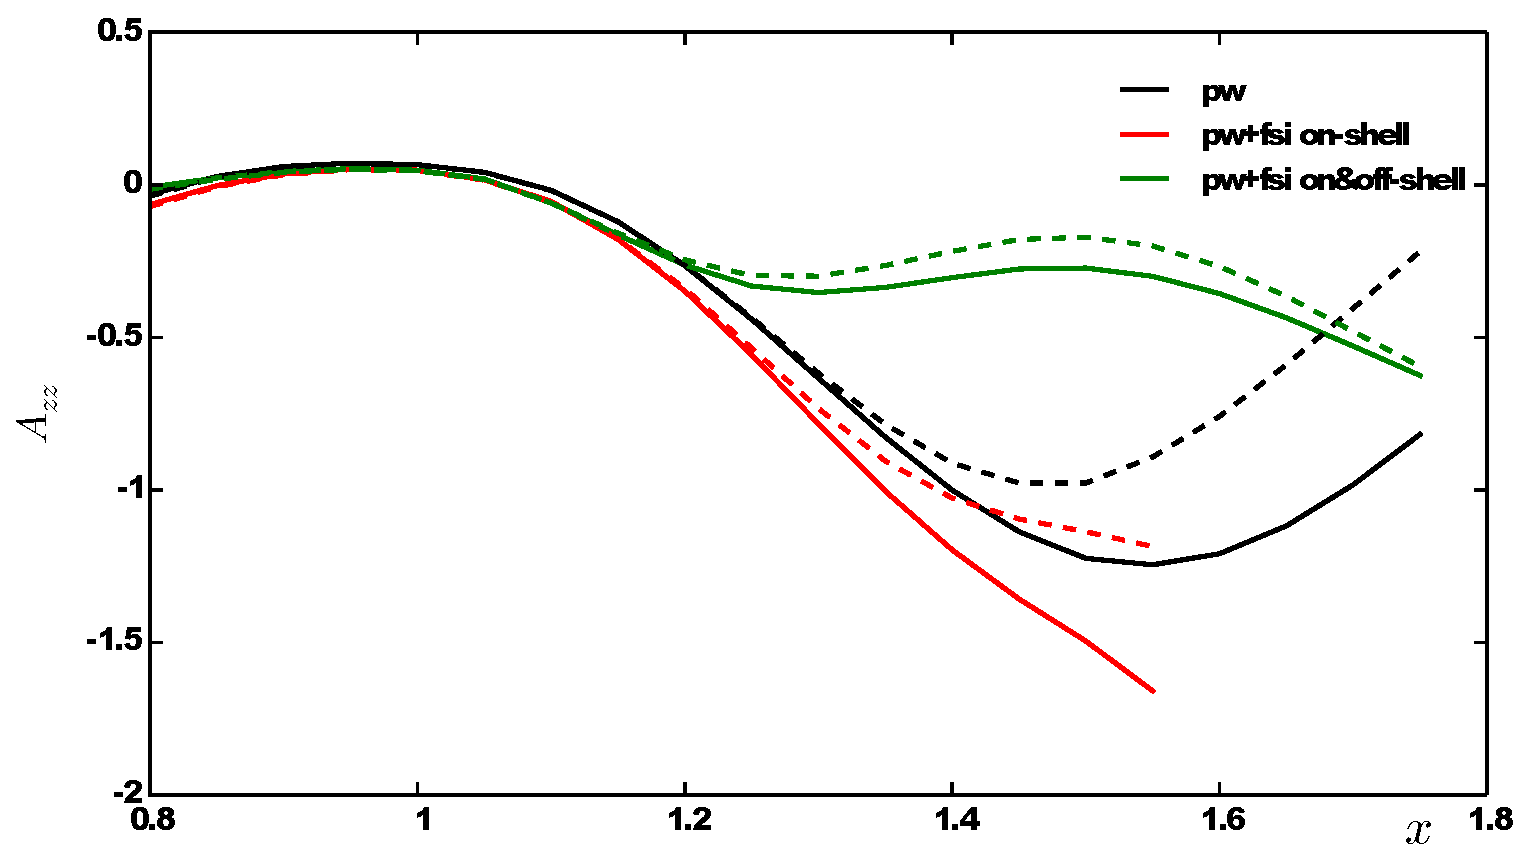
\includegraphics[width=0.5\textwidth]{figs/kin1_cdbonn_av18.eps}
\caption{$A_{zz}$ calculation for $E_0=8.8\mathrm{~GeV}^2$ and $Q^2=1.5\mathrm{~(GeV/}c)^2$ including contributions from final state interactions.  
Solid curves were calculated using the CDBonn deuteron wave function, dashed curves using the AV18 
deuteron wave function.}
\label{fig:fsi-kin1}       % Give a unique label
\end{center}
\end{figure}

\begin{figure}[htb]
\begin{center}
  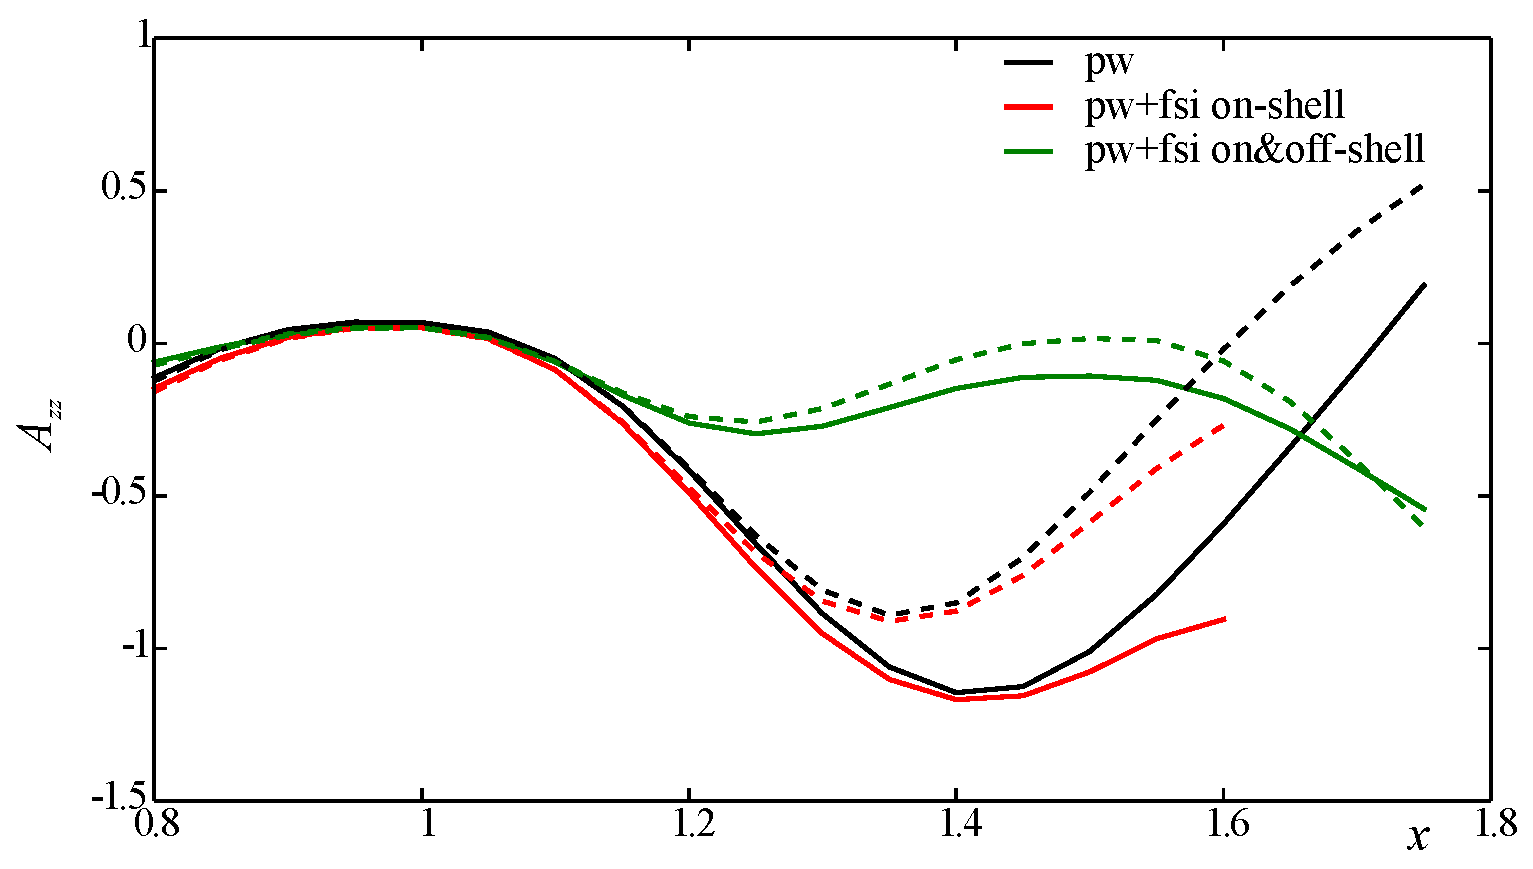
\includegraphics[width=0.5\textwidth]{figs/kin2_cdbonn_av18.eps}
\caption{Same as Fig.~\ref{fig:fsi-kin1}, but for $E_0=8.8\mathrm{~GeV}^2$ and $Q^2=2.9\mathrm{~(GeV/}c)^2$.}
\label{fig:fsi-kin2}       % Give a unique label
\end{center}
\end{figure}

%Note: strange bumps in the red curves (plane-wave+on-shell fsi) is due to contributions almost cancelling each other in combination with numerical errors.  Which means the numerical noise gets enhanced bigtime.  I suggest dropping these for now, since the off-shell contribution dominates anyway.

\iffalse
Most theory calculations calculate Azz with a deuteron polarized along the  virtual photon momentum direction as this limits the number of response  functions included in the cross section.  For a deuteron polarized along the  electron beam direction, an extra rotation of the deuteron density matrix needs  to be accounted for and extra response functions contribute~\cite{Cosyn:2014sqa}.  The next figures show how $A_{zz}$ changes  when accounting for this.

\begin{figure}[htb]
\begin{center}
  \includegraphics[width=0.5\textwidth]{figs/beampol_av18_kin1.eps}
\caption{$A_{zz}$ calculation for kinematic S1 including FSI contributions 
using the AV18 wave function.  
Full curves use have a deuteron polarized along the photon direction, dashed 
ones along the electron beam.}
\label{fig:beampol1}       % Give a unique label
\end{center}
\end{figure}

\begin{figure}[htb]
\begin{center}
  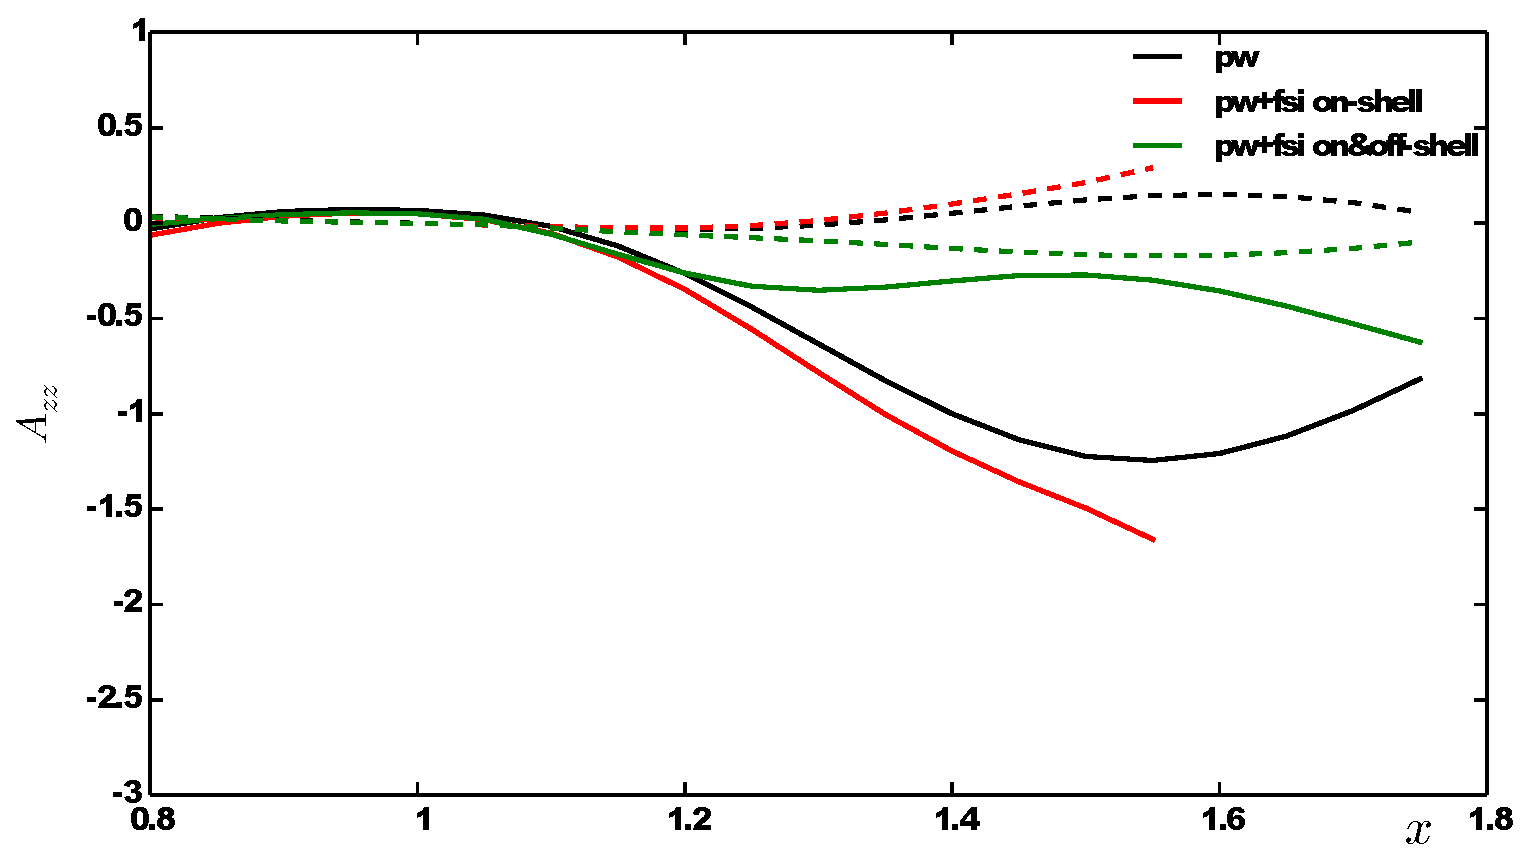
\includegraphics[width=0.5\textwidth]{figs/beampol_cdbonn_kin1.eps}
\caption{Same as Fig.~\ref{fig:beampol1}, but for cdbonn wave function.}
\label{fig:beampol2}       % Give a unique label
\end{center}
\end{figure}

\begin{figure}[htb]
\begin{center}
  \includegraphics[width=0.5\textwidth]{figs/beampol_av18_kin1.eps}
\caption{Same as Fig.~\ref{fig:beampol1}, but H1 kinematics and AV18 wave 
function.}
\label{fig:beampol3}       % Give a unique label
\end{center}
\end{figure}

\begin{figure}[htb]
\begin{center}
  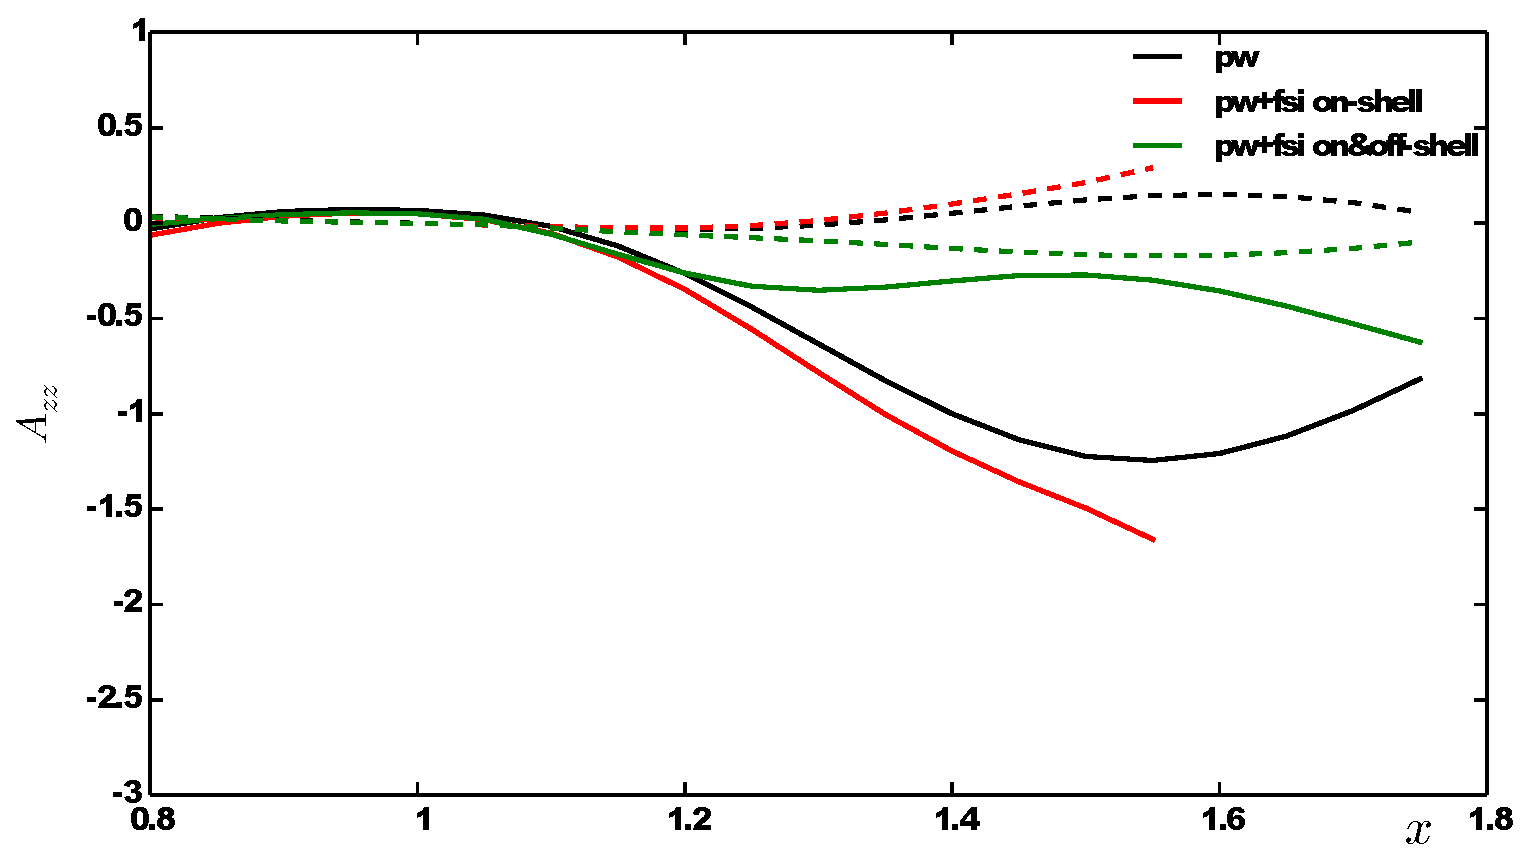
\includegraphics[width=0.5\textwidth]{figs/beampol_cdbonn_kin1.eps}
\caption{Same as Fig.~\ref{fig:beampol1}, but H1 kinematics and cdbonn wave 
function.}
\label{fig:beampol4}       % Give a unique label
\end{center}
\end{figure}
\fi



\subsection{Interest from Theorists}

The measurement proposed has stirred interest in a number of theorists who either have provided or are currently working on calculations. Many of these are on-going and are expected to be completed in the coming year.

The light cone and virtual nucleon calculations of M.~Sargsian~\cite{misak-convo} and M.~Strikman~\cite{strikman-convo} are already available for $A_{zz}$ and are presented in this document. Calculations have been done with difference NN potentials and have found significant differences at large $x$.

Continuing his interest from DIS $b_1$ calculations~\cite{Cosyn:2014sqa}, W.~Cosyn has developed calculations of the quasi-elastic contribution to inclusive deuteron scattering, which will be the dominant contribution in the $x>1$ regime~\cite{cosyn-convo}. His calculations, which include final-state interactions, have been modified to include $A_{zz}$ and are presented in this proposal.

Although not completed at the time of submission, W. Van Orden has calculations in progress using different nucleon-nucleon potentials, as well as different prescriptions for handling the reactions mechanisms in the low $Q^2$ region for tensor polarization observables. In his words, ``Recent studies have shown that it is extremely challenging to disentangle reaction mechanisms from nucleon-nucleon potential effects using cross section information~\cite{Ford:2014yua}. This group is now in the process of extending their studies to vector and tensor asymmetries. Previous low $Q^2$ measurements seemed to indicate that the asymmetries are far less sensitive to reaction 
mechanisms than the cross sections~\cite{Passchier:2001uc}; so while the 
new calculations are not yet available, it is clear that the asymmetries will produce unique constraints 
on our understanding of the deuteron."~\cite{vanorden-convo}

G.~A.~Miller~\cite{miller-convo} has developed an interest in this measurement, and is working on calculations that involve 6-quark effects in the elastic region. In his own words, he states ``This proposal really challenges theorists to better understand the meaning of nuclear wave functions in a situation that demands a relativistic treatment. I plan on working to understand this reaction during the upcoming summer."

S.~Liuti also affirms the importance of understanding the structure of the deuteron in the kinematics presented in this proposal, stating ``This is an important measurement and should be calculated more thoroughly."~\cite{liuti-convo}


% Similar calculations have recently been done for the approved D($e,e'p)n$ at high $Q^2$, high $p_m$ experiment~\cite{Ford:2014yua}. 

In summary, we are encouraged that several theorists have been and continue to be engaged in serious efforts to calculate $A_{zz}$ in the $x>1$ region using a variety of models.

\section{$T_{20}$ Motivation}

[[ Need to fill in background information on $T_{20}$ ]]

\section{The Proposed Experiment}

We propose to measure the tensor asymmetry $A_{zz}$ and tensor analyzing power $T_{20}$ from inclusive electron scattering from polarized deuterons in the quasi-elastic and elastic region of $\XMIN<x<\XMAX$, $\QMIN$~(GeV/$c)^2 < Q^2 <\QMAX$~(GeV/$c)^2$, and $\WMIN < W_{NN} < \WMAX$~GeV using the Hall C HMS and SHMS spectrometers at forward angle from a solid polarized ND$_3$ target.


\subsection{$A_{zz}$ Experimental Method} %Measurement of $A_{zz}$ }

The measured double differential cross section for electron scattering from a spin-1 target is characterized by a vector polarization $P_{z}$ and tensor polarization $P_{zz}$. With an unpolarized beam and the target field oriented along the beam, the cross section is expressed as~\cite{Leidemann:1991qs}
\begin{equation}
\frac{d^2\sigma_p}{d\Omega dE'}=\frac{d^2\sigma_u}{d\Omega dE'}\left(1+\frac{1}{2}P_{zz}A_{zz}) \right),
\label{eq:one}
\end{equation}
where $\sigma_p$ ($\sigma_u$) is the polarized (unpolarized) cross section and $A_{zz}$ is the
tensor asymmetry of the virtual-photon deuteron cross section.  This allows us to write
the polarized tensor asymmetry with positive tensor polarization using an unpolarized electron beam as
\begin{eqnarray}
\label{Azz}
A_{zz} = \frac{2}{P_{zz}}\left(\frac{\sigma_p - \sigma_u}{\sigma_u}\right).
\end{eqnarray}
The tensor polarization is given by 
\begin{equation}
P_{zz}=(p_++p_-)-2p_0,
\end{equation}
where $p_m$ represents the population in the $m_J=+1$,~$-1$,~or $0$ state.

Eq. \ref{Azz} reveals that the asymmetry $A_{zz}$ compares two different cross sections measured under different polarization conditions of the target: positively tensor polarized and unpolarized.  
To obtain the relative cross section measurement in the same configuration, the same target cup and material will be used at alternating polarization states (polarized vs. unpolarized),  and the magnetic field providing the quantization axis will be oriented along the beamline at all times.
This field will always be held at the same value, regardless of the target material polarization state. 
This process, identical to that used for the already-approved $b_1$ measurement~\cite{b1prop}, ensures that the acceptance remains consistent within the stability of the super conducting magnet.  


Since many of the factors involved in the cross sections cancel in
the ratio, Eq. \ref{Azz} can be expressed in terms 
of the charge normalized, efficiency corrected numbers of tensor polarized ($N_p$) and unpolarized ($N_u$) counts, 
\begin{eqnarray} \label{3}
A_{zz}&=&\frac{2}{fP_{zz}}\left(\frac{N_p - N_u}{N_u}\right) .
\end{eqnarray}

The dilution factor $f$ corrects for the presence of unpolarized nuclei in the target and is defined by
\begin{equation}
f=\frac{N_D\sigma_D}{N_N\sigma_N+N_D\sigma_D+\sum\limits_{A} N_A\sigma_A},
\end{equation}
where $N_D$ is the number of deuterium nuclei in the target and $\sigma_D$ is the corresponding inclusive double differential scattering cross 
section, $N_N$ is the nitrogen number of scattered nuclei with cross section $\sigma_N$, and $N_A$ is the number of other scattering nuclei of mass number $A$ with cross section $\sigma_A$. As has been noted in previous work~\cite{Frankfurt:1988nt}, the dilution factor at high $x$ drops off considerably until the SRC plateau region, as shown in Fig.~\ref{fdil}. By using a high-luminosity solid target at a small scattering angle $\theta_{e'}$, this effect will be counteracted. The dilution factor is a much smaller problem for elastic deuteron scattering at $x=2$.

\begin{figure}
\begin{center}
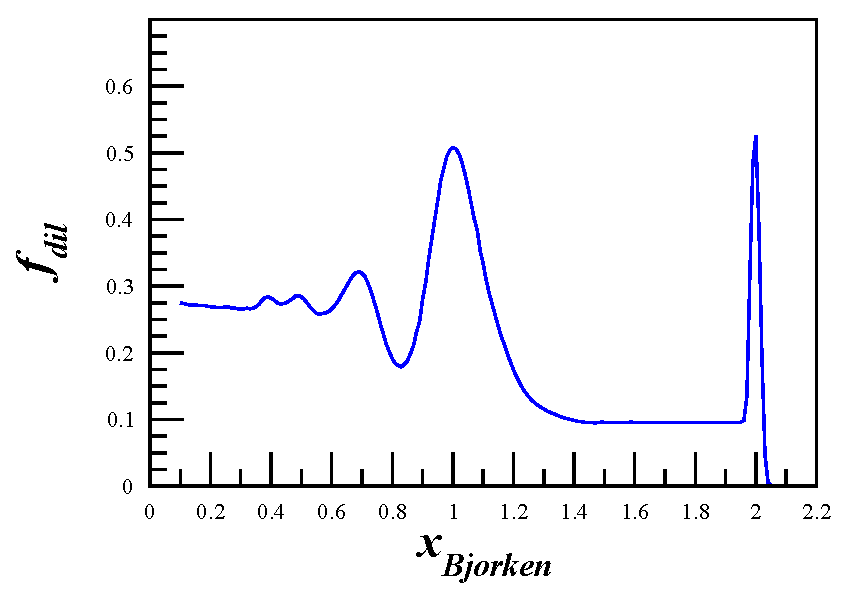
\includegraphics[width=0.45\textwidth]{figs/fdil_q2_15.eps}
\caption{\label{fdil}The estimated dilution factor, in this case at $Q^2=1.5 \mathrm{~(GeV}/c)^2$, is expected to drop off at high $x$ until it reaches the SRC plateau region and then the elastic peak at $x=2$. The low dilution factor of $1.1<x<1.95$ will be counteracted by using a high-luminosity target.}
\end{center}
\end{figure}

The dilution factor can be written in terms of the relative volume ratio of ND$_3$ to LHe in the target cell, otherwise known as the packing fraction $p_f$.  
In our case of a cylindrical target cell oriented along the magnetic field,the packing fraction is exactly equivalent to the percentage of the cell length filled with ND$_3$.  
%The dilution factor is discussed in further detail in Sec. \ref{dil}.

If the time is evenly split between scattering off of polarized and unpolarized ND$_3$, the time necessary to achieve the desired precision $\delta A$ is:
\begin{equation}
t=\frac{N_p}{R_p}+\frac{N_u}{R_u}=\frac{8}{f^2P_{zz}^2}\left(\frac{R_p(R_u+R_p)}{R_u^3}\right)\frac{1}{\delta A_{zz}^2}
\end{equation} 
where $R_{p(u)}$ is the polarized (unpolarized) rate and $N_{p(u)}$ is the total estimated 
number of polarized (unpolarized) counts to achieve the uncertainty $\delta A_{zz}$.  

%See Sec.~\ref{stat} for full details of the statistical uncertainty.


\subsection{$T_{20}$ Experimental Method} %Measurement of $A_{zz}$ }
\label{t20_exp}

A measurement of $T_{20}$ will be extracted from $A_{zz}$ on the elastic peak for each $Q^2$ mentioned in Section~\ref{kinematics}. We will follow the method described by the NIKHEF measurements~\cite{Bouwhuis:1998re}, which also used a tensor polarized target. Our methods differ in that we will use the high resolution of the HMS and SHMS to determine the elastic peak through kinematic cuts, where NIKHEF utilized a second spectrometer for that purpose. 
%It should also be noted that the Boden measurement used a beam current of $<0.4$~nA. The current for these proposed $T_{20}$ measurements at \CURRENT~nA is $200\times$ the exploratory Boden measurement.

The analyzing powers of a tensor-polarized target are described by the cross-section
\begin{equation}
\sigma = \sigma_0\left[ 1 + \frac{A_d^T P_{zz}}{\sqrt{2}} \right],
\label{cs-ana}
\end{equation}
where
\begin{equation} A^T_d = \sum_{i=0}^{2}d_{2i}T_{2i}
\end{equation}
and
\begin{equation} d_{20} = \frac{3 \cos^2 \theta^* -1}{2},~~d_{21} = -\sqrt{\frac{3}{2}}\sin2\theta^*\cos\phi^*,~~d_{22}=\sqrt{\frac{3}{2}}\sin^2\theta^*\cos 2\phi^*.
\end{equation}
$\theta^*$ and $\phi^*$ are in the frame where the $z$ axis is along the $\vec{q}$ and the $x$ axis is perpendicular to $z$ in the scattering plane, as described in~\cite{Donnelly:1985ry} and shown in Fig.~\ref{coords}. For this proposal, $\theta^* \approx 70^{\circ}$ and $\phi^* \approx 0^{\circ}$, as our target field will be oriented along the beamline and $\theta_{\vec{q}}\approx 70^{\circ}$ on the elastic peak.

\begin{figure}
\begin{center}
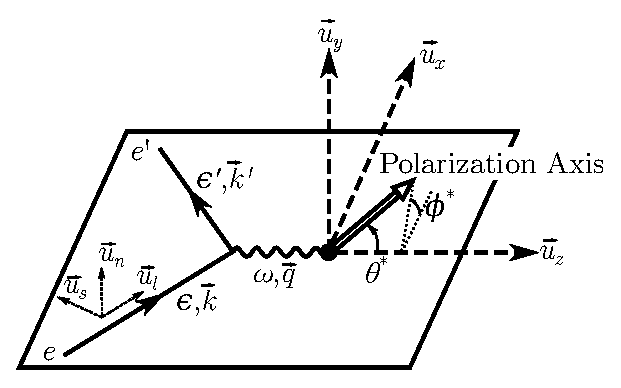
\includegraphics[width=0.4\textwidth]{figs/coordinate_system.eps} 
\caption{\label{coords}Coordinate system used in determining the tensor analyzing powers.
}
\end{center}
\end{figure}

%If that's the case, the $d_{21}\approx -0.787,~~d_{22}\approx 1.08~~$ and $d_{20} \approx -0.3245$.

We rearrange Eq.~\ref{cs-ana} to be defined as our observable $A_{zz} = \frac{2}{P_{zz}}\left( \frac{\sigma}{\sigma_0} - 1 \right)$,
\begin{equation}A_{zz} = \sqrt{2} \left[ d_{20} T_{20} + d_{21} T_{21} + d_{22} T_{22}\right],
\end{equation}
\begin{equation}
T_{20} = \frac{A_{zz}}{d_{20}\sqrt{2}}-\frac{d_{21}}{d_{20}}T_{21}-\frac{d_{22}}{d_{20}}T_{22}.
\end{equation}
Contributions from $T_{21}$ and $T_{22}$ are expected to be small but not negligible, and will be calculated from models that best match world data. Uncertainties from $T_{21}$ and $T_{22}$ are expected to be $10\%$ and are included within the $T_{20}$ systematic calculations.




\subsection{Kinematics}
\label{kinematics}

\label{EXP}
We propose to measure the tensor asymmetry $A_{zz}$ for $\XMIN<x<\XMAX$, $\QMIN$~(GeV/$c)^2 < Q^2 <\QMAX$~(GeV/$c)^2$, and $\WMIN < W_{NN} < \WMAX$~GeV and extract the tensor analyzing power $T_{20}$ for $\QMINT20$~(GeV/$c)^2 < Q^2 <\QMAXT20$~(GeV/$c)^2$. Central kinematics of the spectrometers are given in Table~\ref{RATES1}
%, estimates for the uncertainties of $A_{zz}$ are given in Tables~\ref{RATES2}-\ref{RATES3}, and estimates for the uncertainties of $T_{20}$ are given in Table\need
. Fig.~\ref{kincov} shows the planned kinematic coverage utilizing the Hall C HMS and SHMS spectrometers at forward angles. 

\begin{table}
\begin{center}
\begin{tabular}{cc|c|c|c|c|c|c}
 & & $E_0$ & $Q^2$    	& $E'$  &    $\theta_{e'}$  &  Rates   & PAC Time   \\
%& (GeV) & (GeV$^2$)  & (GeV)  &     (deg.)   &   (kHz)  & (hours) \\
& & (GeV) & (GeV$^2$)  & (GeV)  &     ($^{\circ}$)   &   (kHz)  & (Days) \\
%\multicolumn{2}{|c|}{$\times 10^{-2}$}
\hline\hline
SHMS & (S1) & 8.8	&  1.5	&  8.36	&    8.2  	&    0.38	&   25 \\
HMS  & (H1) & 8.8	&  2.9	&  7.26	&    12.2	&    0.04	&   25 \\  
SHMS & (S2) & 6.6	&  0.7	&  6.35	&    7.5 	&    3.57	&   8 \\
HMS  & (H2) & 6.6	&  1.8	&  5.96	&    12.3	&    0.09	&   8 \\  
SHMS & (S3) & 2.2	&  0.2	&  2.15	&    10.9 	&    10.5	&   1 \\
HMS  & (H3) & 2.2	&  0.3	&  2.11	&    14.9	&    3.23	&   1 \\  
\hline\hline
\end{tabular}
\caption{\label{RATES1}Summary of the central kinematics and physics rates using the Hall C  spectrometers.}
\end{center}
\end{table}









\begin{figure}
\begin{center}
%\includegraphics[width=\textwidth]{figs/Pzz_30_all_q2_w.eps}
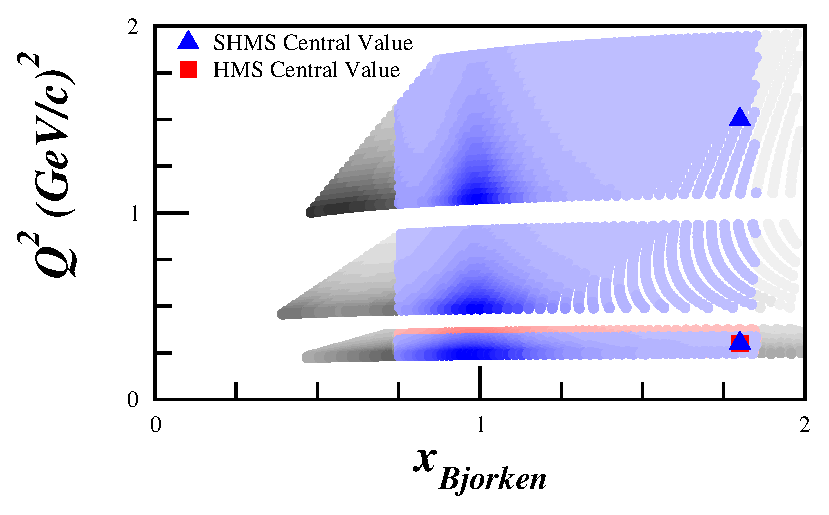
\includegraphics[width=0.49\textwidth]{figs/Pzz_30_all_q2.eps}

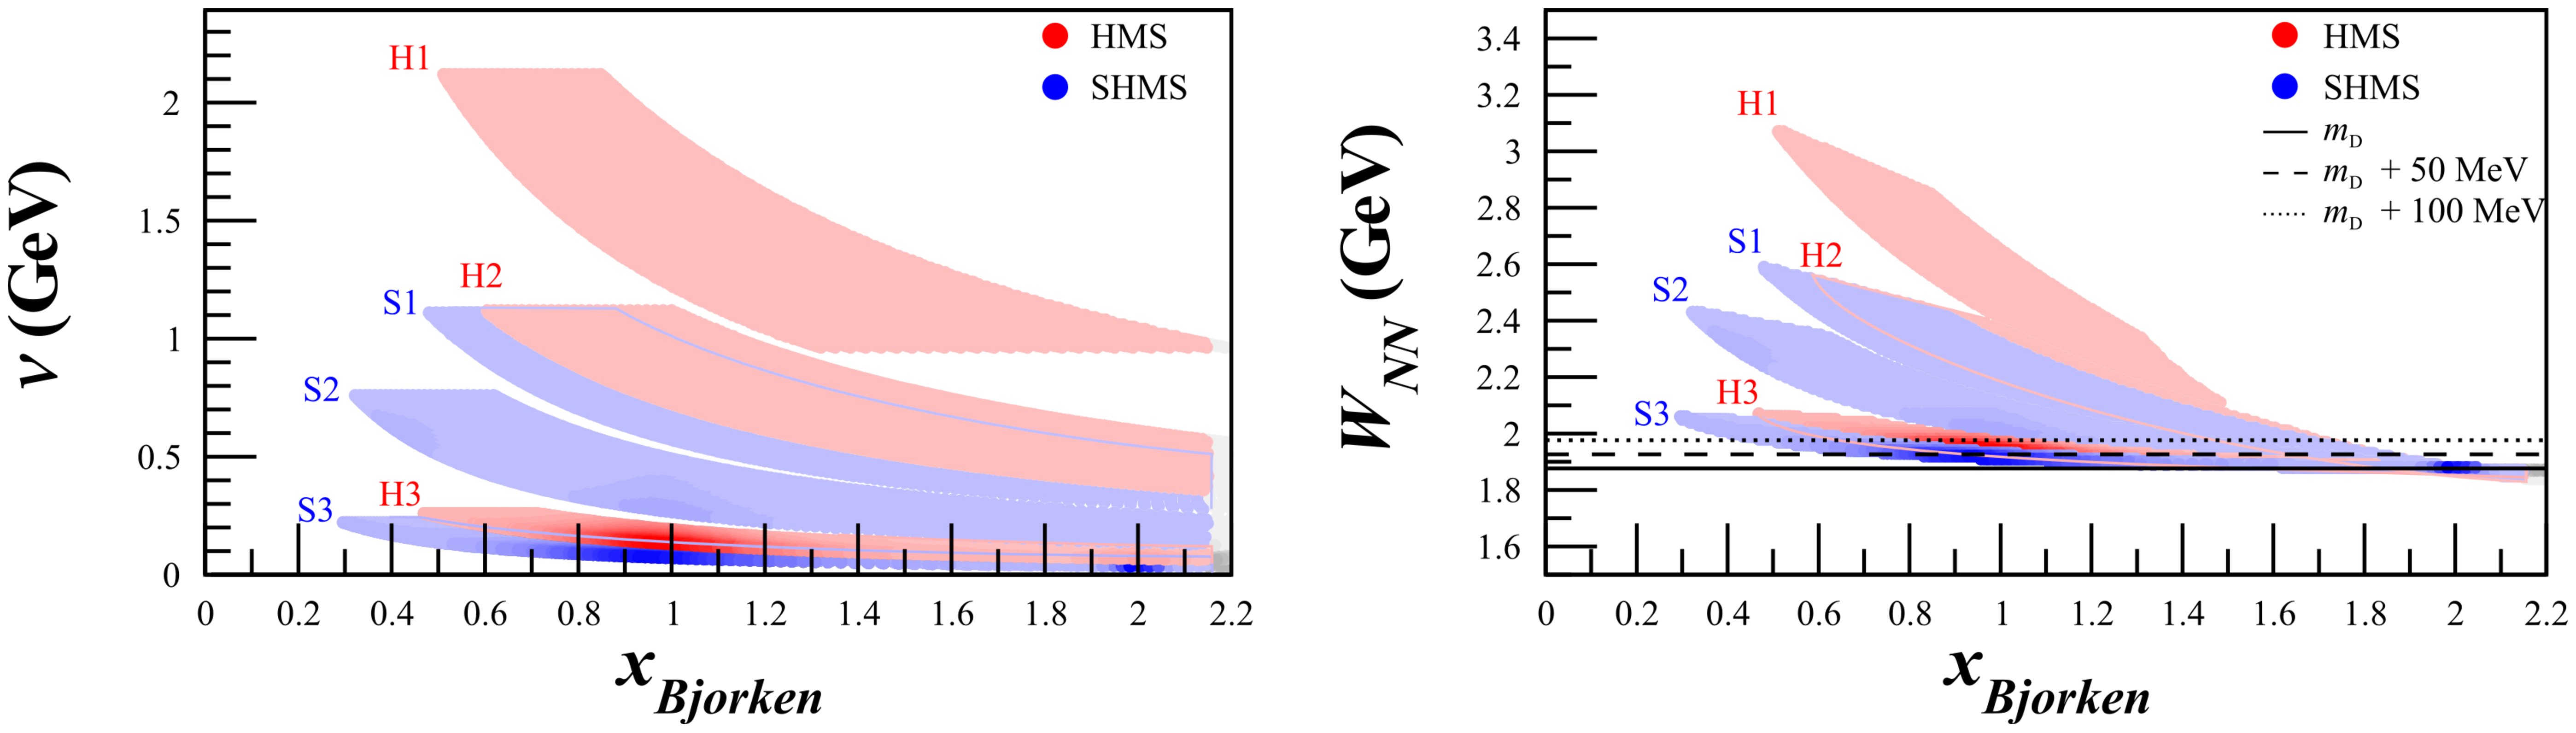
\includegraphics[width=\textwidth]{figs/Pzz_30_all_nu_wnn.eps}
%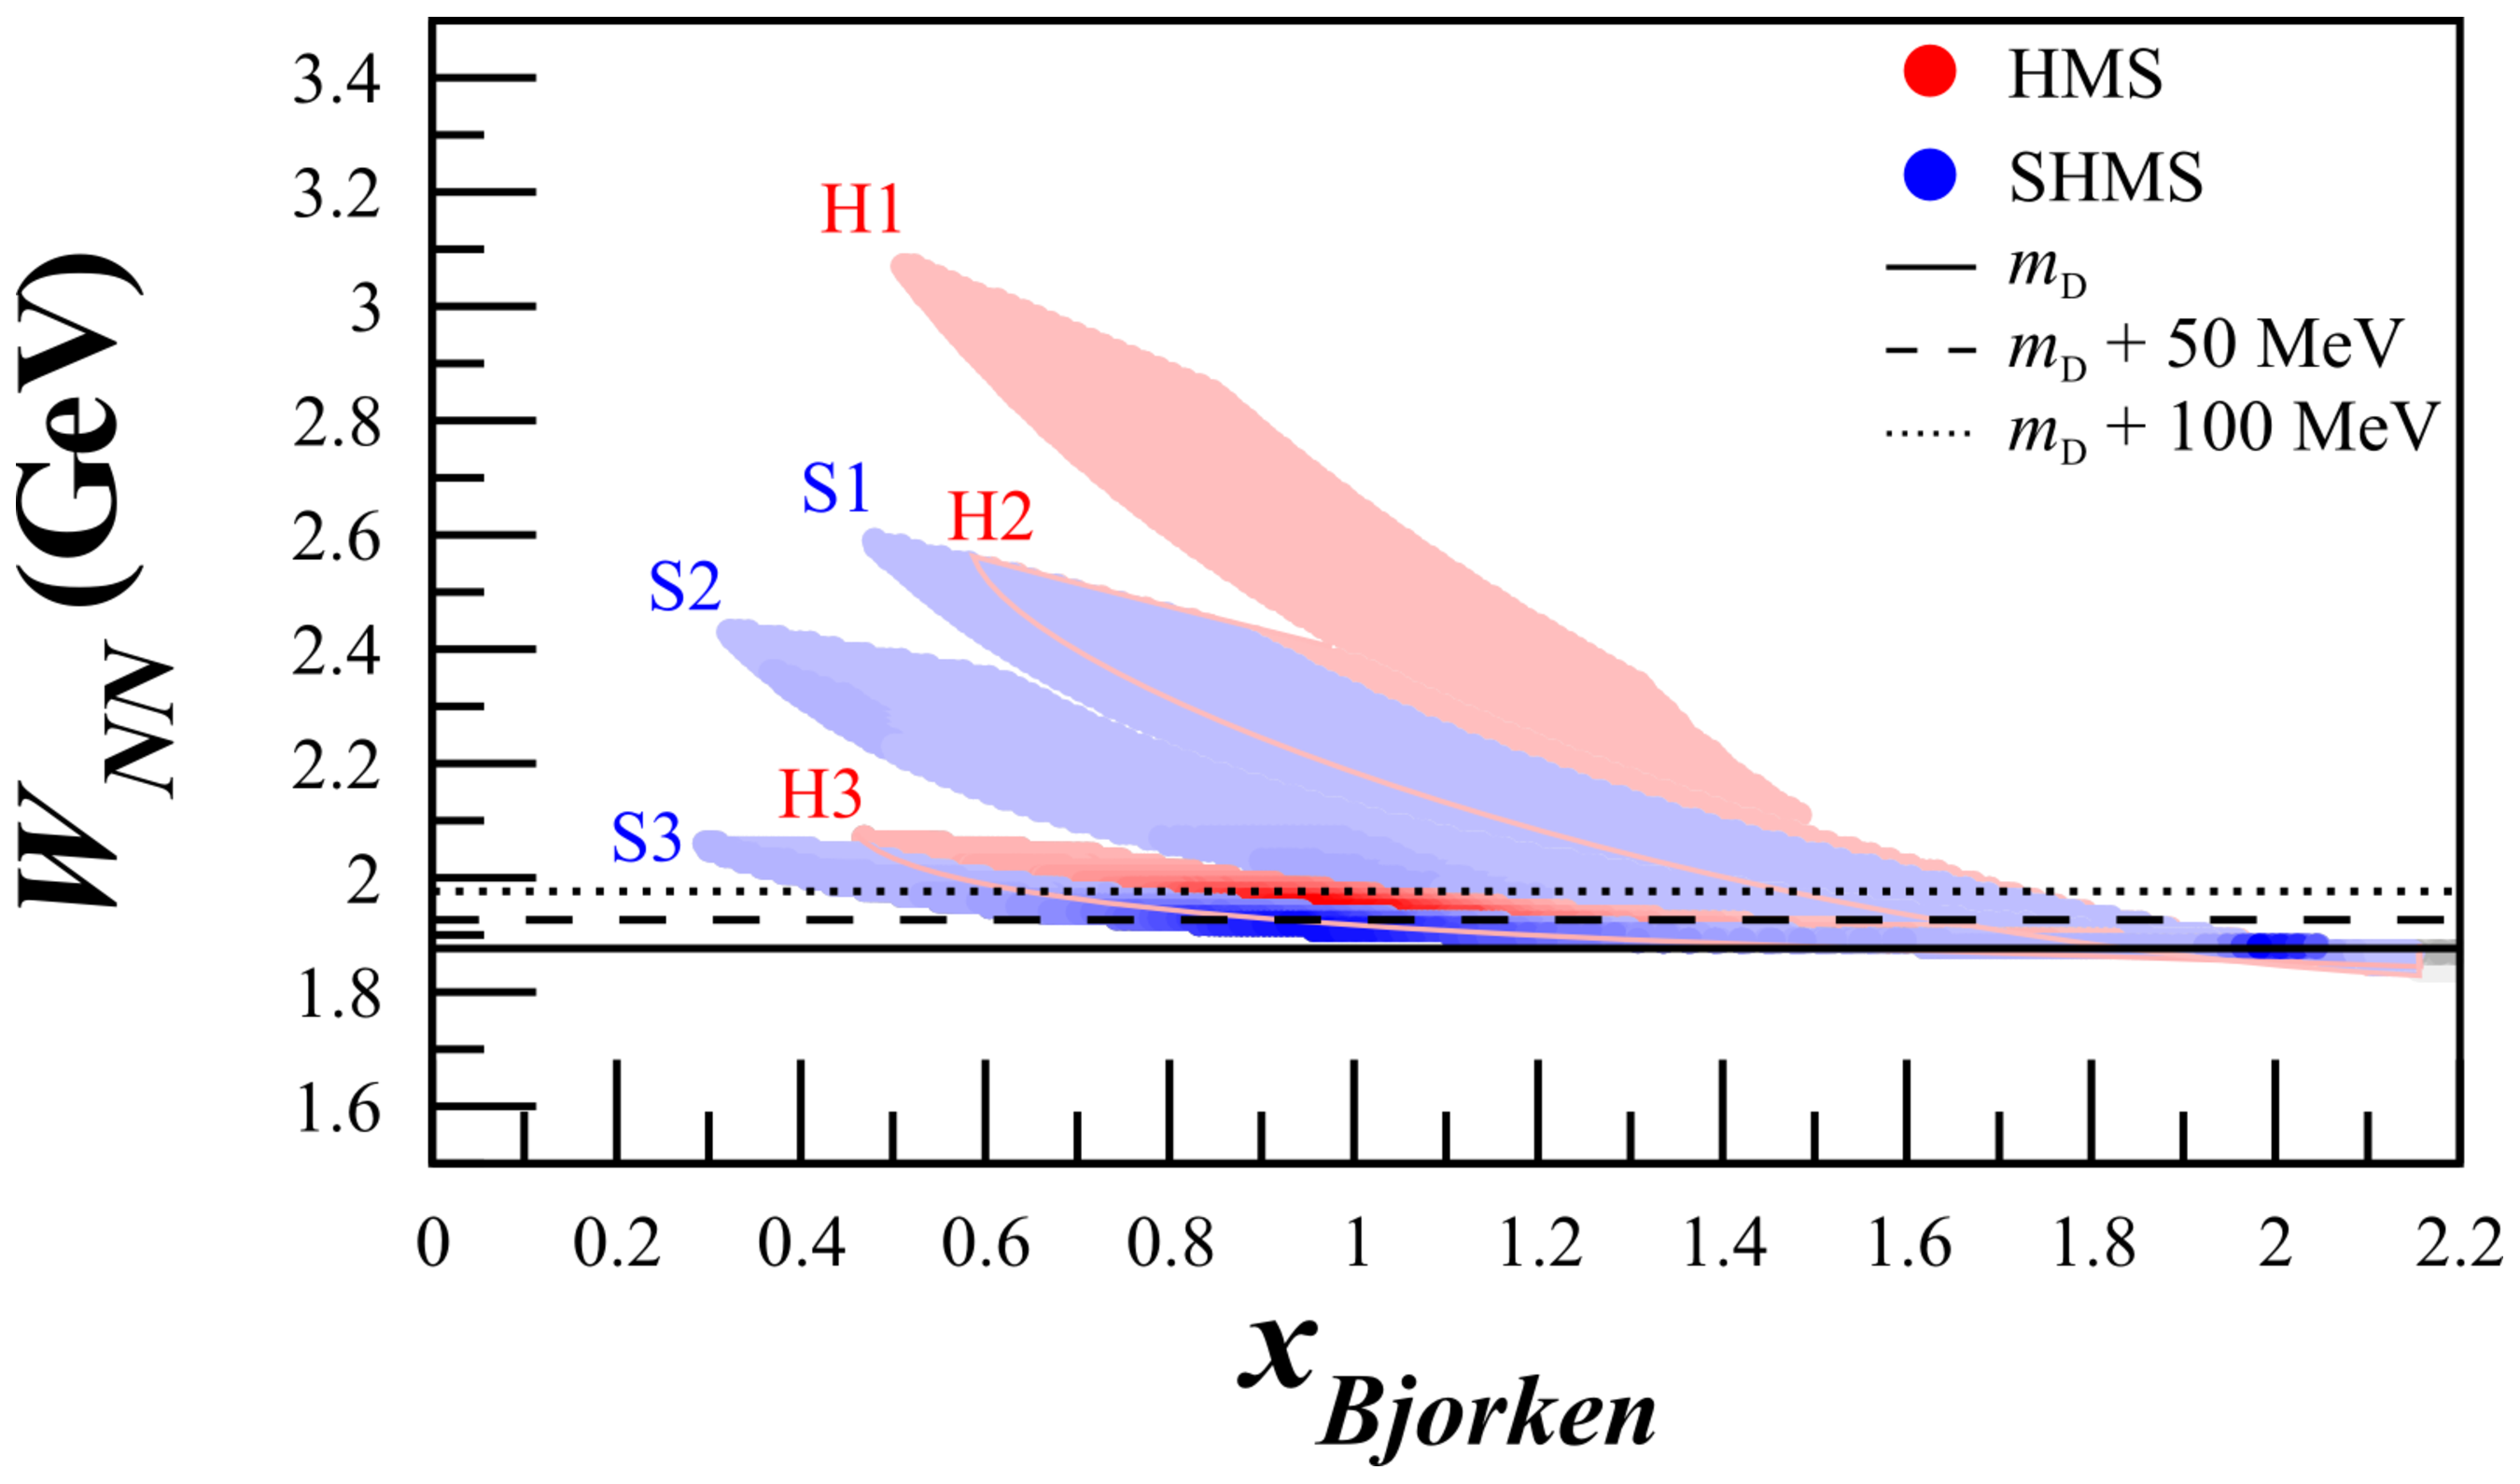
\includegraphics[width=0.49\textwidth]{figs/Pzz_30_all_wnn.eps} %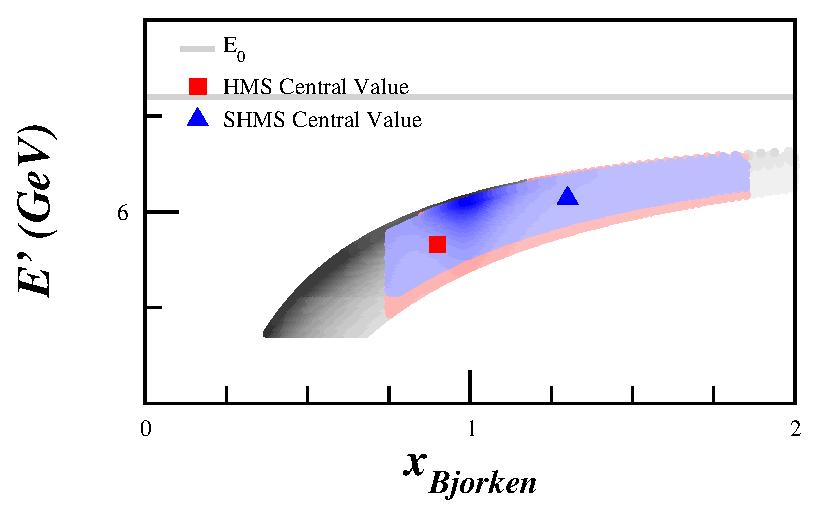
\includegraphics[width=0.49\textwidth]{figs/kine/Pzz_30_eprime.eps}
%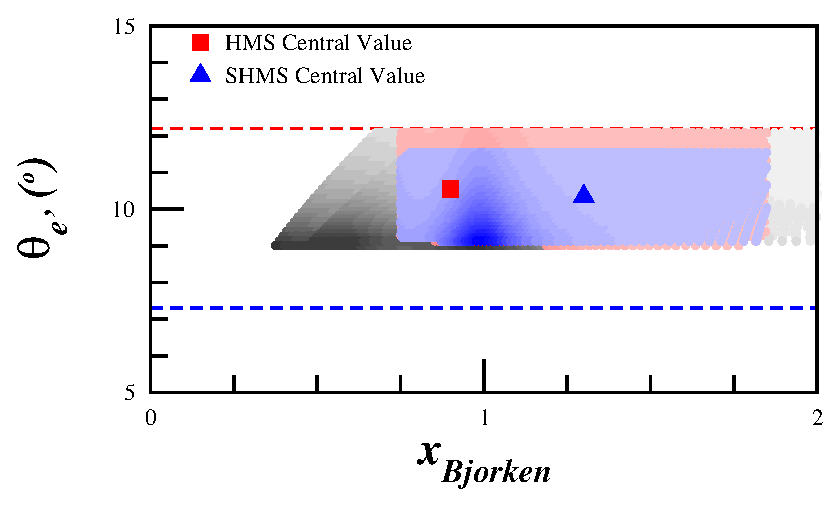
\includegraphics[width=0.49\textwidth]{figs/kine/Pzz_30_theta_eprime.eps}~~ 

\caption{\label{kincov} Kinematic coverage for central spectrometer settings at $Q^2=2.9~(\mathrm{GeV}/c)^2$ (H1), $1.8~(\mathrm{GeV}/c)^2$ (H2), $1.5~(\mathrm{GeV}/c)^2$ (S1), $0.7~(\mathrm{GeV}/c)^2$ (S2), $0.3~(\mathrm{GeV}/c)^2$ (H3), and $0.2~(\mathrm{GeV}/c)^2$ (S3). The grey regions are not included in our statistics estimates since they fall outside the range of electron-deuteron scattering. Darker shading represents areas with higher statistics. The solid, dashed, and dotted lines in the $W_{NN}$ plot indicate deuteron mass, deuteron mass + 50 MeV, and deuteron mass + 100 MeV, respectively. Virtual-nucleon and light cone calculations are only valid for $W_{NN}>m_D+50$~MeV.}
\end{center}
\end{figure}

Although it has been pointed out that the current construction of the SHMS constrains it to angles $>10\%$ due to fringe fields affecting the beam entering the dump~\cite{Moore:2014sxa}, this can be resolved in a number of ways. As discussed in \cite{Moore:2014sxa}, passive iron shielding can be installed within the SHMS that would not affect the target field. Additionally, given the low beam current proposed, a local beam dump could be installed immediately following the target. In the worst case, we could meet the physics motivation by keeping the same $Q^2$ ranges as S1, S2, and S3 but lowering the highest beam energies while putting the SHMS at larger angles. In this case, the HMS would be used at very similar angles to combine statistics between the spectrometers to make up for the loss in statistics from the SHMS. 


The polarized \TARGET target is discussed in Section~\ref{POLTARGSEC}.  The magnetic field of the target will be held constant along the beamline at all times, while the target state is alternated between a polarized and unpolarized state.
The tensor polarization and packing fraction used in the rates estimate are \PZZ\% and \PF, respectively. 
The dilution factor in the range of this measurement is shown in Fig.~\ref{fdil_plot}. The spread of the elastic peak for the dilution factor was calculated assuming a momentum resolution of $0.1\%$ for the HMS and $0.08\%$ for the SHMS.
With an incident electron beam current of \CURRENT nA, the expected deuteron luminosity is \LUMI.


%$1.57\times 10^{35}$~cm$^{-2}}$s$^{-1}$.
%$?.??\times 10^{35}$~cm$^{-2}$s$^{-1}$.

\begin{figure}
\begin{center}
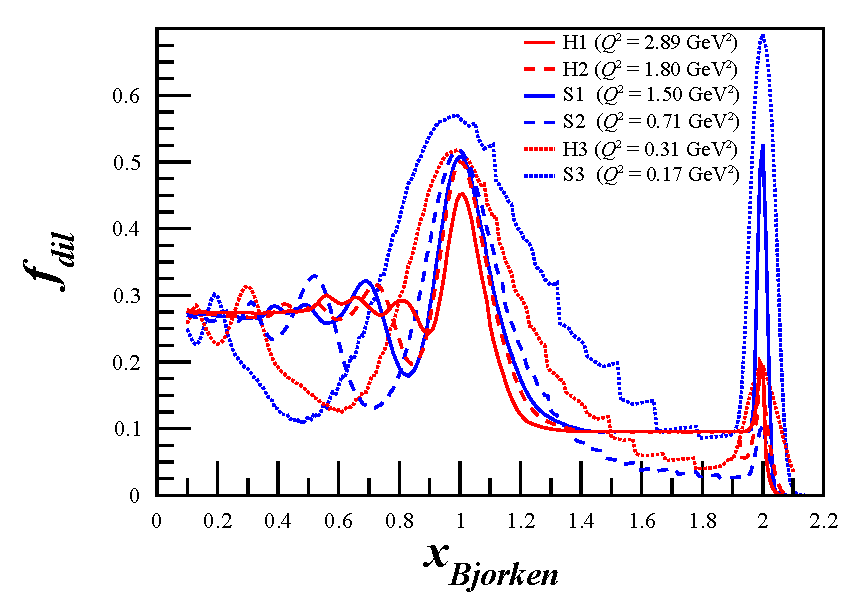
\includegraphics[width=0.65\textwidth]{figs/Pzz_30_fdil_all.eps} 
\caption{\label{fdil_plot}Projected dilution factor covering the entire $x$ range to be measured using a combination of P. Bosted's~\cite{Bosted:2012qc} and M. Sargsian's~\cite{misak-convo} code, along with a calculation of the elastic peak using a parametrization of the deuteron form factors, for the SHMS and HMS.}
\end{center}
\end{figure}


The momentum bite and the acceptance were assumed to be $\Delta P = \pm 8\%$ and $\Delta\Omega = 5.6$~msr for the HMS, and $\Delta P= ^{+20\%}_{-8\%}$ 
%$-8<\Delta P <+20\%$
and $\Delta\Omega =4.4$~msr for the SHMS. 
%
For the choice of the kinematics,
special attention was taken onto the angular and momentum limits of the spectrometers with a longitudinal polarized target: for the
HMS, $12.2^{\circ} \le \theta \le 85^{\circ}$ and $1 \le P_0 \le 7.3$ GeV/c, and for the SHMS,
$5.5^{\circ} \le \theta \le 40^{\circ}$ and $2 \le P_0 \le 11$ GeV/c. In addition, the
opening angle between the spectrometers is physically constrained to be larger than 17.5$^{\circ}$.

A total of \productiondays days of beam time is requested for production data, with an additional \overheaddays days of expected overhead. The expected uncertainties, described in detail in Section~\ref{uncertainties}, are given in Tables~\ref{RATES2}-\ref{RATES-T20} and Figs.~\ref{PROJ}-\ref{PROJ-T20}.

\begin{table}
\begin{center}
\begin{tabular}{c|ccc|ccc|ccc}
 ~ & \multicolumn{3}{|c}{H1: $Q^2=2.9\mathrm{~(GeV/}c)^2$} & \multicolumn{3}{|c}{H2: $Q^2=1.8\mathrm{~(GeV/}c)^2$} & \multicolumn{3}{|c}{S1: $Q^2=1.5\mathrm{~(GeV/}c)^2$} \\
 \hline
  $x$  & $f_{dil}$ & $\delta A_{zz}^{stat}$ & $\delta A_{zz}^{sys}$ & $f_{dil}$ & $\delta A_{zz}^{stat}$ & $\delta A_{zz}^{sys}$ & $f_{dil}$ & $\delta A_{zz}^{stat}$ & $\delta A_{zz}^{sys}$ \\
  &     & $\times 10^{-2}$  & $\times 10^{-2}$  &    & $\times 10^{-2}$  & $\times 10^{-2}$ &    & $\times 10^{-2}$  & $\times 10^{-2}$ \\
\hline\hline
%       |         Q2=2.9         |      Q2=1.8           |      Q2=1.5
%  x  	   fdil 	   dAzz	 dAzzSys  fdil 	  dAzz   dAzzSys  fdil   dAzz	 dAzzSys
 0.50   &  0.29	 & 2.02	& 1.84	& ---	& ---	& ---	& 0.25	& 0.72	& 1.84 \\
 0.60   &  0.29	 & 0.91	& 0.10	& 0.27	& 3.15	& 0.10	& 0.30	& 0.36	& 0.10 \\ 
 0.70   &  0.27	 & 1.01	& 0.10	& 0.32	& 1.26	& 0.10	& 0.29	& 0.38	& 0.10 \\
 0.80	&  0.30	 & 1.11	& 1.34	& 0.20	& 2.00	& 0.48	& 0.17	& 0.74	& 1.34 \\
 0.90	&  0.24	 & 1.73 	& 0.38 	& 0.27	& 1.45	& 1.10	& 0.29	& 0.44	& 0.38 \\
 1.00	&  0.46	 & 1.03	& 0.10 	& 0.50	& 0.74	& 0.10	& 0.51	& 0.24	& 0.10 \\
 1.10	&  0.28	 & 2.48	& 0.14 	& 0.33	& 1.58	& 1.65	& 0.34	& 0.49	& 0.14 \\
 1.20	&  0.09	 & 11.7	& 1.55 	& 0.10	& 7.18	& 3.31	& 0.17	& 1.34	& 1.55 \\
 1.30	&  0.11	 & 16.8	& 4.13 	& 0.11	& 9.76	& 4.96	& 0.12	& 2.79	& 4.13 \\
 1.40	&  ---	 & ---	& --- 	& 0.12	& 15.1	& 6.65	& 0.13	& 4.30	& 6.72 \\
 1.50	&  ---	 & ---	& ---	& 0.11	& 19.8	& 8.29	& 0.10	& 7.01	& 8.34 \\
 1.60	&  ---	 & ---	& --- 	& ---	& ---	& ---	& 0.10	& 9.60	& 8.42 \\
 1.70	&  ---	 & ---	& --- 	& ---	& ---	& ---	& 0.10	& 12.7	& 7.04 \\
 1.80	&  ---	 & ---	& --- 	& ---	& ---	& ---	& 0.10	& 16.6	& 4.72 \\
 2.00   &  ---	 & ---	& ---	& 0.20	& 9.33	& 9.20	& 0.50	& 2.79	& 9.20 \\
\hline\hline
\end{tabular}
\caption{\label{RATES2}Summary of the expected uncertainty for each $x$ bin for settings S1, H1, and H2. }
\end{center}
\end{table}

\begin{table}
\begin{center}
\begin{tabular}{c|ccc|ccc|ccc}
 ~ & \multicolumn{3}{|c}{S2: $Q^2=0.7\mathrm{~(GeV/}c)^2$} & \multicolumn{3}{|c}{H3: $Q^2=0.3\mathrm{~(GeV/}c)^2$} & \multicolumn{3}{|c}{S3: $Q^2=0.2\mathrm{~(GeV/}c)^2$} \\
 \hline
  $x$  & $f_{dil}$ & $\delta A_{zz}^{stat}$ & $\delta A_{zz}^{sys}$ & $f_{dil}$ & $\delta A_{zz}^{stat}$ & $\delta A_{zz}^{sys}$ & $f_{dil}$ & $\delta A_{zz}^{stat}$ & $\delta A_{zz}^{sys}$ \\
  &     & $\times 10^{-2}$  & $\times 10^{-2}$  &    & $\times 10^{-2}$  & $\times 10^{-2}$ &    & $\times 10^{-2}$  & $\times 10^{-2}$ \\
\hline\hline
%       |         Q2=0.7         |      Q2=0.3           |      Q2=0.2
%  x  	   fdil 	   dAzz	 dAzzSys  fdil 	  dAzz   dAzzSys  fdil   dAzz	 dAzzSys
 0.30   &  0.24	 & 0.99	& 1.84	& ---	& ---	& ---	& 0.18	& 2.13	& 1.84 \\
 0.40   &  0.28	 & 0.26	& 1.84	& ---	& ---	& ---	& 0.12	& 1.38	& 1.84 \\
 0.50   &  0.32	 & 0.21	& 1.84	& 0.14	& 3.52	& 1.84	& 0.11	& 1.23	& 1.84 \\
 0.60   &  0.19	 & 0.41	& 0.10	& 0.12	& 2.26	& 0.10	& 0.18	& 0.78	& 0.10 \\ 
 0.70   &  0.13	 & 0.68	& 0.10	& 0.18	& 1.33	& 0.10	& 0.28	& 0.48	& 0.10 \\
 0.80	&  0.19	 & 0.48	& 0.48	& 0.30	& 0.72	& 0.48	& 0.42	& 0.31	& 0.48 \\
 0.90	&  0.39	 & 0.22 	& 1.10 	& 0.46	& 0.45	& 1.10	& 0.54	& 0.24	& 1.10 \\
 1.00	&  0.52	 & 0.16	& 0.10 	& 0.52	& 0.43	& 0.10	& 0.58	& 0.25	& 0.10 \\
 1.10	&  0.39	 & 0.28	& 1.27 	& 0.43	& 0.63	& 1.07	& 0.53	& 0.33	& 0.95 \\
 1.20	&  0.22	 & 0.65	& 2.54 	& 0.30	& 1.15	& 2.14	& 0.40	& 0.55	& 1.91 \\
 1.30	&  0.14	 & 1.34	& 3.81 	& 0.19	& 2.16	& 3.22	& 0.32	& 0.83	& 2.87 \\
 1.40	&  0.09	 & 2.29	& 5.06 	& 0.14	& 3.52	& 4.29	& 0.24	& 1.31	& 3.82 \\
 1.50	&  0.06	 & 4.09	& 6.35	& 0.10	& 5.85	& 5.37	& 0.20	& 1.86	& 4.78 \\
 1.60	&  0.04	 & 7.76	& 7.60 	& 0.06	& 10.4	& 6.45	& 0.14	& 2.87	& 5.74 \\
 1.70	&  0.04	 & 9.23	& 8.88 	& 0.05	& 13.5	& 7.52	& 0.10	& 4.53	& 6.69 \\
 1.80	&  0.03	 & 14.9	& 9.20 	& 0.06	& 13.9	& 8.60	& 0.11	& 4.73	& 7.66 \\
 2.00   &  0.67	 & 3.79	& 9.20	& 0.20	& 3.05	& 9.20	& 0.70	& 0.45	& 9.20 \\
\hline\hline
\end{tabular}
\caption{\label{RATES3}Summary of the expected uncertainty for each $x$ bin for settings S2, S3, and H3. }
\end{center}
\end{table}


\begin{figure}
\begin{center}
%\includegraphics[width=0.45\textwidth]{figs/plots0705/b1_proj_newmiller_lin.eps}
%\hspace{0.5cm}
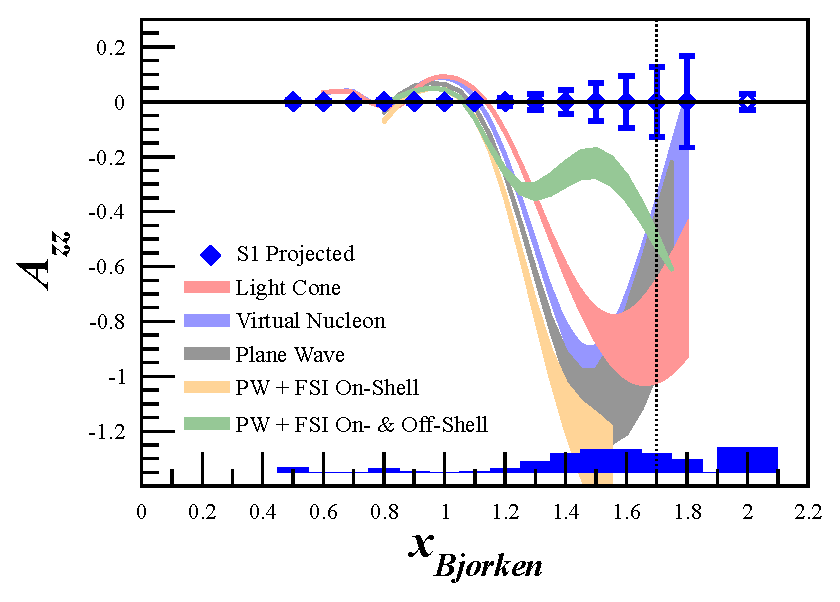
\includegraphics[width=0.49\textwidth]{figs/Azz_S1.eps}
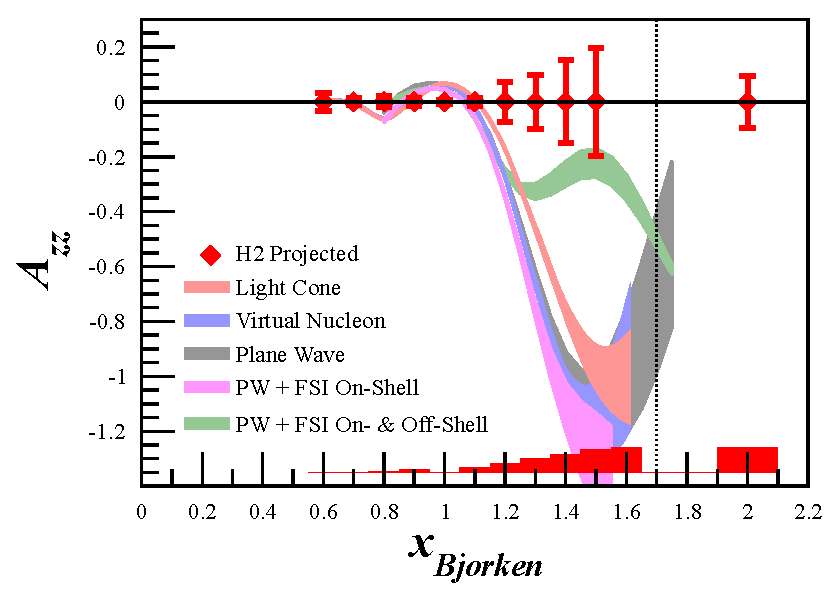
\includegraphics[width=0.49\textwidth]{figs/Azz_H2.eps}
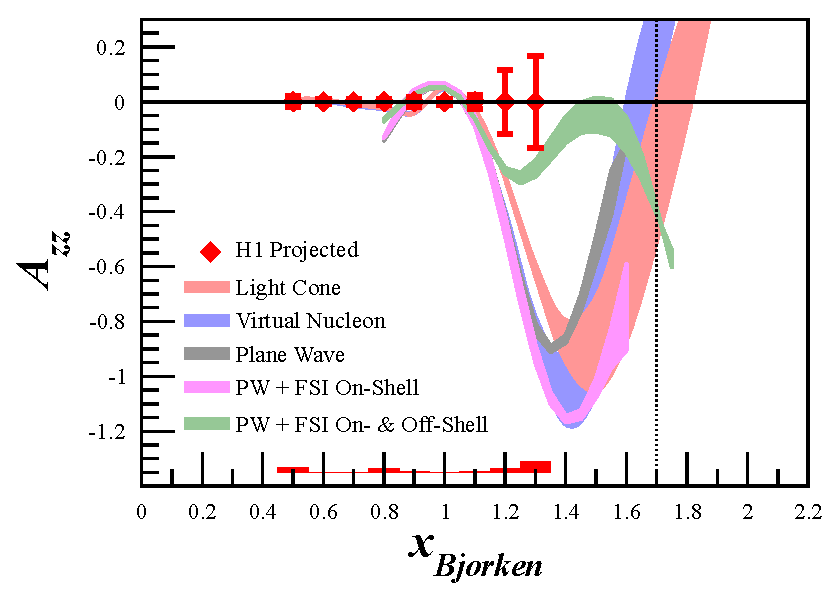
\includegraphics[width=0.49\textwidth]{figs/Azz_H1.eps}
 %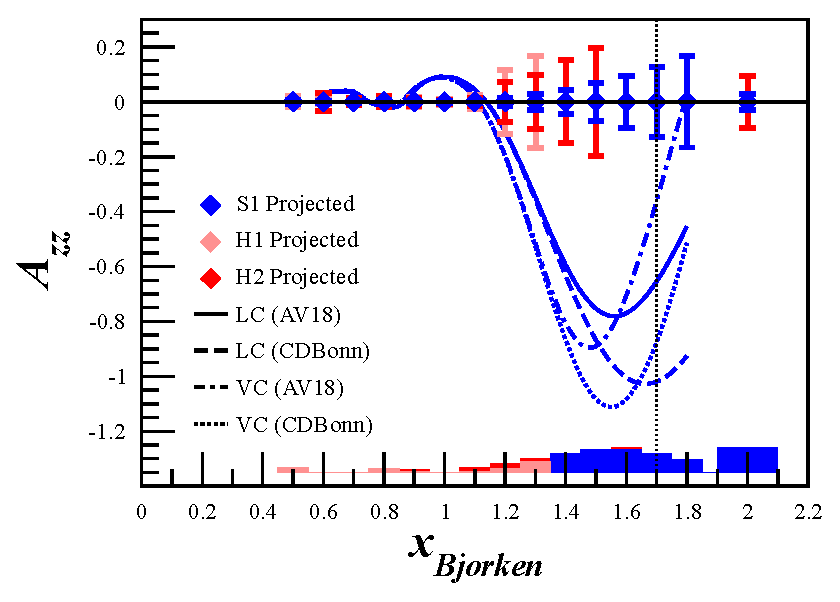
\includegraphics[width=0.49\textwidth]{figs/Azz_S1_H1_H2_vn_lc.eps} 
%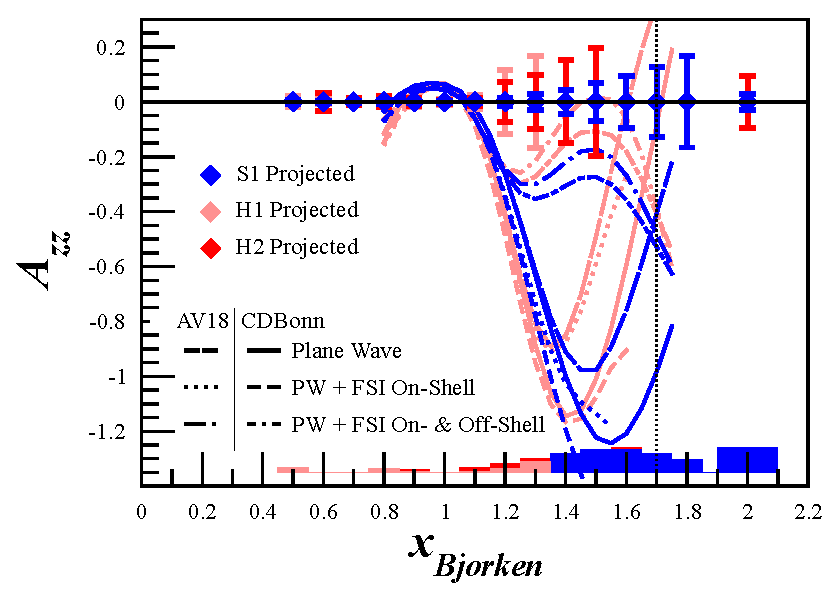
\includegraphics[width=0.49\textwidth]{figs/Azz_S1_H1_H2_fsi.eps} \\
\includegraphics[width=0.49\textwidth]{figs/Azz_S2_H3_S3.eps} 
\caption{\label{PROJ}Projected uncertainties for the tensor asymmetry $A_{zz}$ with \productiondays days of beam time for SHMS settings S1, S2, and S3, and HMS settings H1, H2, and H2 as described in Table~\ref{RATES1}. The bottom band represents the systematic uncertainty. The bands for the theoretical calculations show the spread based on the choice of NN potentials. The upper $x$ limit for H1 (H2) is $x=1.3$ ($x=1.5$). Light-cone (LC) and virtual-nucleon (VN) calculations using the AV18 and CDBonn potentials were provided by M. Sargsian~\cite{Sargsian:2014fla}. The dotted line at $x=1.75$ indicates the threshold of $W_{NN}>m_D+50$~MeV where LC and VN calculations begin to not be valid as $A_{zz}$ approaches the elastic peak~\cite{Frankfurt:1993sp}. Final state interactions on the virtual-nucleon model were provided by W. Cosyn~\cite{cosyn-convo}, indicating the effects from on- and off-shell. The bottom-right plot includes a modified Frankfurt and Strikman model~\cite{Frankfurt:1988nt} that estimates the peak shifts in $x$ expected due to the SRC scaling changing with $Q^2$~\cite{Frankfurt:2008zv}.
}
\end{center}
\end{figure}

\begin{figure}
\begin{center}
%\includegraphics[width=0.45\textwidth]{figs/plots0705/b1_proj_newmiller_lin.eps}
%\hspace{0.5cm}
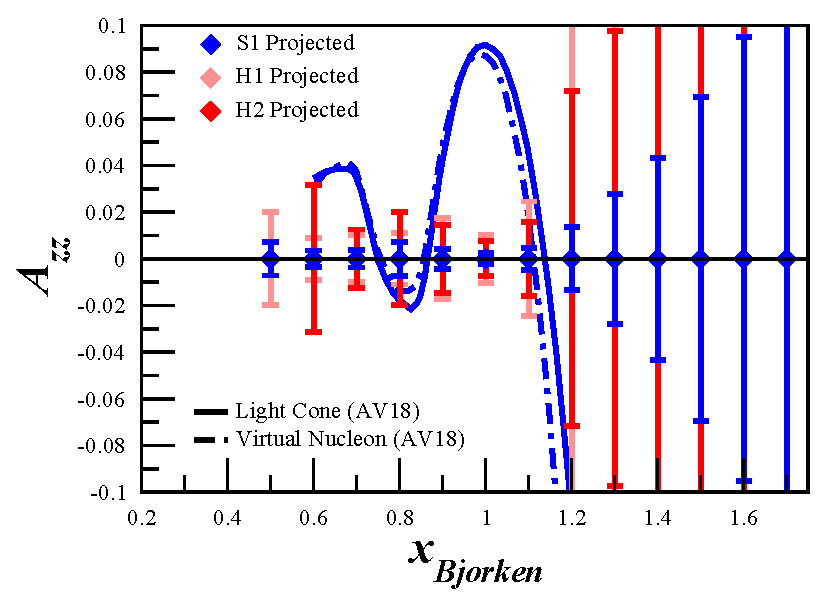
\includegraphics[width=0.49\textwidth]{figs/Azz_S1_H1_H2_zoom.eps} 
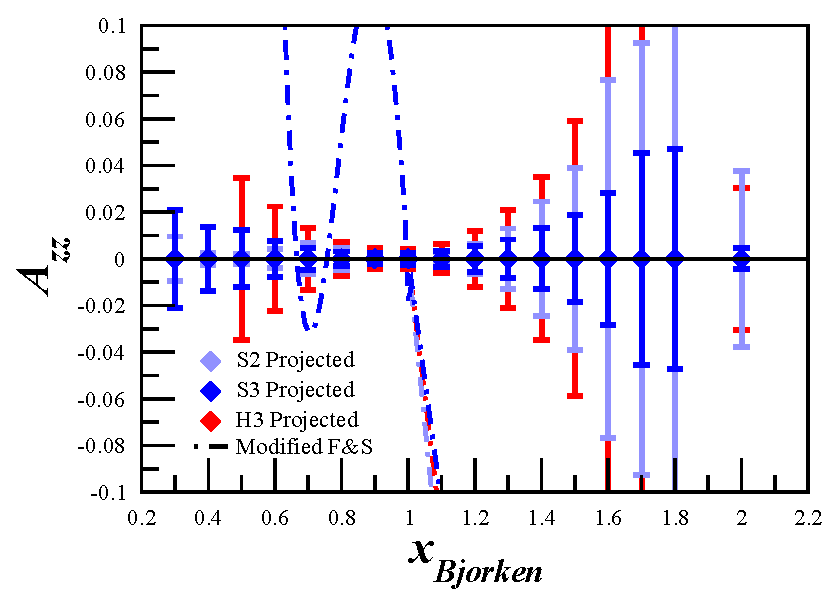
\includegraphics[width=0.49\textwidth]{figs/Azz_S2_H3_S3_zoom.eps} 
\caption{\label{PROJ-zoom}Projected uncertainties for the tensor asymmetry $A_{zz}$ with \productiondays days of beam time, same as in Figure~\ref{PROJ}, but zoomed in to $-0.1<A_{zz}<0.1$ to more clearly show the small uncertainties around the quasi-elastic peak.
}
\end{center}
\end{figure}

\begin{table}
\begin{center}
\begin{tabular}{c|c|c|c}
		& $Q^2$    	& $\delta T_{20}^{stat}$	&  $\delta T_{20}^{sys}$ \\
Setting	& (GeV$^2$)	& $\times 10^{-2}$		& $\times 10^{-2}$ \\
\hline\hline
H2 		& 1.8		&  21.7					& 4.74 \\  
S1 		& 1.5		&  6.09					& 4.77 \\
S2 		& 0.7		&  8.28					& 6.88 \\  
H3 		& 0.3		&  6.66					& 9.91 \\  
S3 		& 0.2		&  0.99					& 5.59 \\
  
\hline\hline
\end{tabular}
\caption{\label{RATES-T20}Expected uncertainties for $T_{20}$ assuming a systematic uncertainty of 9.2\%, which could be reduced further by utilizing the S3 measurement as a calibration for the polarized target.}
\end{center}
\end{table}

\begin{figure}
\begin{center}
%\includegraphics[width=0.45\textwidth]{figs/plots0705/b1_proj_newmiller_lin.eps}
%\hspace{0.5cm}
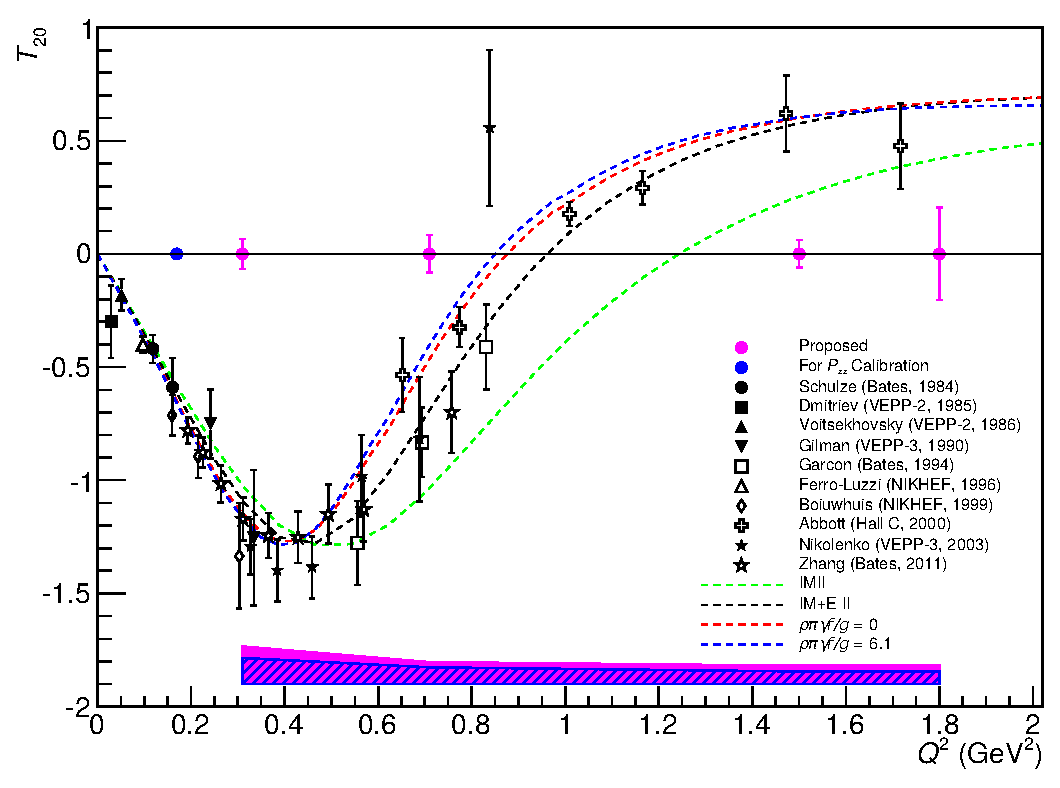
\includegraphics[width=\textwidth]{figs/plot_t20_fit.eps} 
\caption{\label{PROJ-T20}Projected uncertainties for the elastic tensor analyzing power $T_{20}$ with \productiondays days of beam time are shown alongside the world data~\cite{Holt:2012gg}. The point shown in blue, measured at $Q^2=0.2$~GeV$^2$ where $T_{20}$ is well known theoretically and experimentally, will be used as a calibration for $P_{zz}$, and can potentially be used to further reduce the leading systematic uncertainty as indicated by the blue-dashed band.
}
\end{center}
\end{figure}

\iffalse
\subsubsection{SHMS Angular Constraints}

It was recently pointed out that the SHMS is being built such that it would not be able to go to low angles without the magnets interfering with the beam dump~\cite{Moore:2014sxa}. In particular, angles below $\approx10^{\circ}$ would cause the beam to miss the dump. Although solutions have been proposed, including a passive system of adding extra iron to the magnet yokes and beam pipe to reduce field leakage, they have not yet been implemented. In the case that they are not installed by the time of running, we can utilize a slightly different set of kinematics that will cover most of the same $Q^2$ range as in Section~\ref{kinematics} but at lower beam energies and larger angles. Although less ideal, the physics motivation is still valid at the reduced kinematics and the rates still make for a compelling measurement, as shown in Table~\ref{RATES1-const} and Figs.~\ref{kincov-const}-\ref{PROJ-const}.

\begin{table}
\begin{center}
\begin{tabular}{cc|c|c|c|c|c|c}
 & & $E_0$ & $Q^2$    	& $E'$  &    $\theta_{e'}$  &  Rates   & PAC Time   \\
%& (GeV) & (GeV$^2$)  & (GeV)  &     (deg.)   &   (kHz)  & (hours) \\
& & (GeV) & (GeV$^2$)  & (GeV)  &     ($^{\circ}$)   &   (kHz)  & (Days) \\
%\multicolumn{2}{|c|}{$\times 10^{-2}$}
\hline\hline
% Spec  Set   E_0       Q^2      E'        Th         Rate      Time
SHMS & (S1') & 6.6	&  1.5	&  6.07	&    11.1  	&    0.13	&   25 \\
HMS  & (H1') & 6.6	&  1.8	&  5.96	&    12.3	&    0.09	&   25 \\  
%SHMS & (S2) & 4.4	&  0.6	&  4.20	&    10.1 	&    2.07	&   8 \\
SHMS & (S2') & 4.4	&  0.7	&  4.15	&    11.3 	&    0.90	&   8 \\
HMS  & (H2') & 4.4	&  0.8	&  4.11	&    12.2	&    0.80	&   8 \\
SHMS & (S3') & 2.2	&  0.2	&  2.15	&    10.9 	&    10.5	&   1 \\
HMS  & (H3') & 2.2	&  0.3	&  2.11	&    14.9	&    3.23	&   1 \\  
\hline\hline
\end{tabular}
\caption{\label{RATES1-const}Central kinematics if the SHMS is constrained to $>10^{\circ}$. The lowest settings (S3 and H3) are unchanged from Fig.~\ref{RATES1}.}
\end{center}
\end{table}

%


\begin{figure}
\begin{center}
%\includegraphics[width=\textwidth]{figs/Pzz_30_all_q2_w.eps}
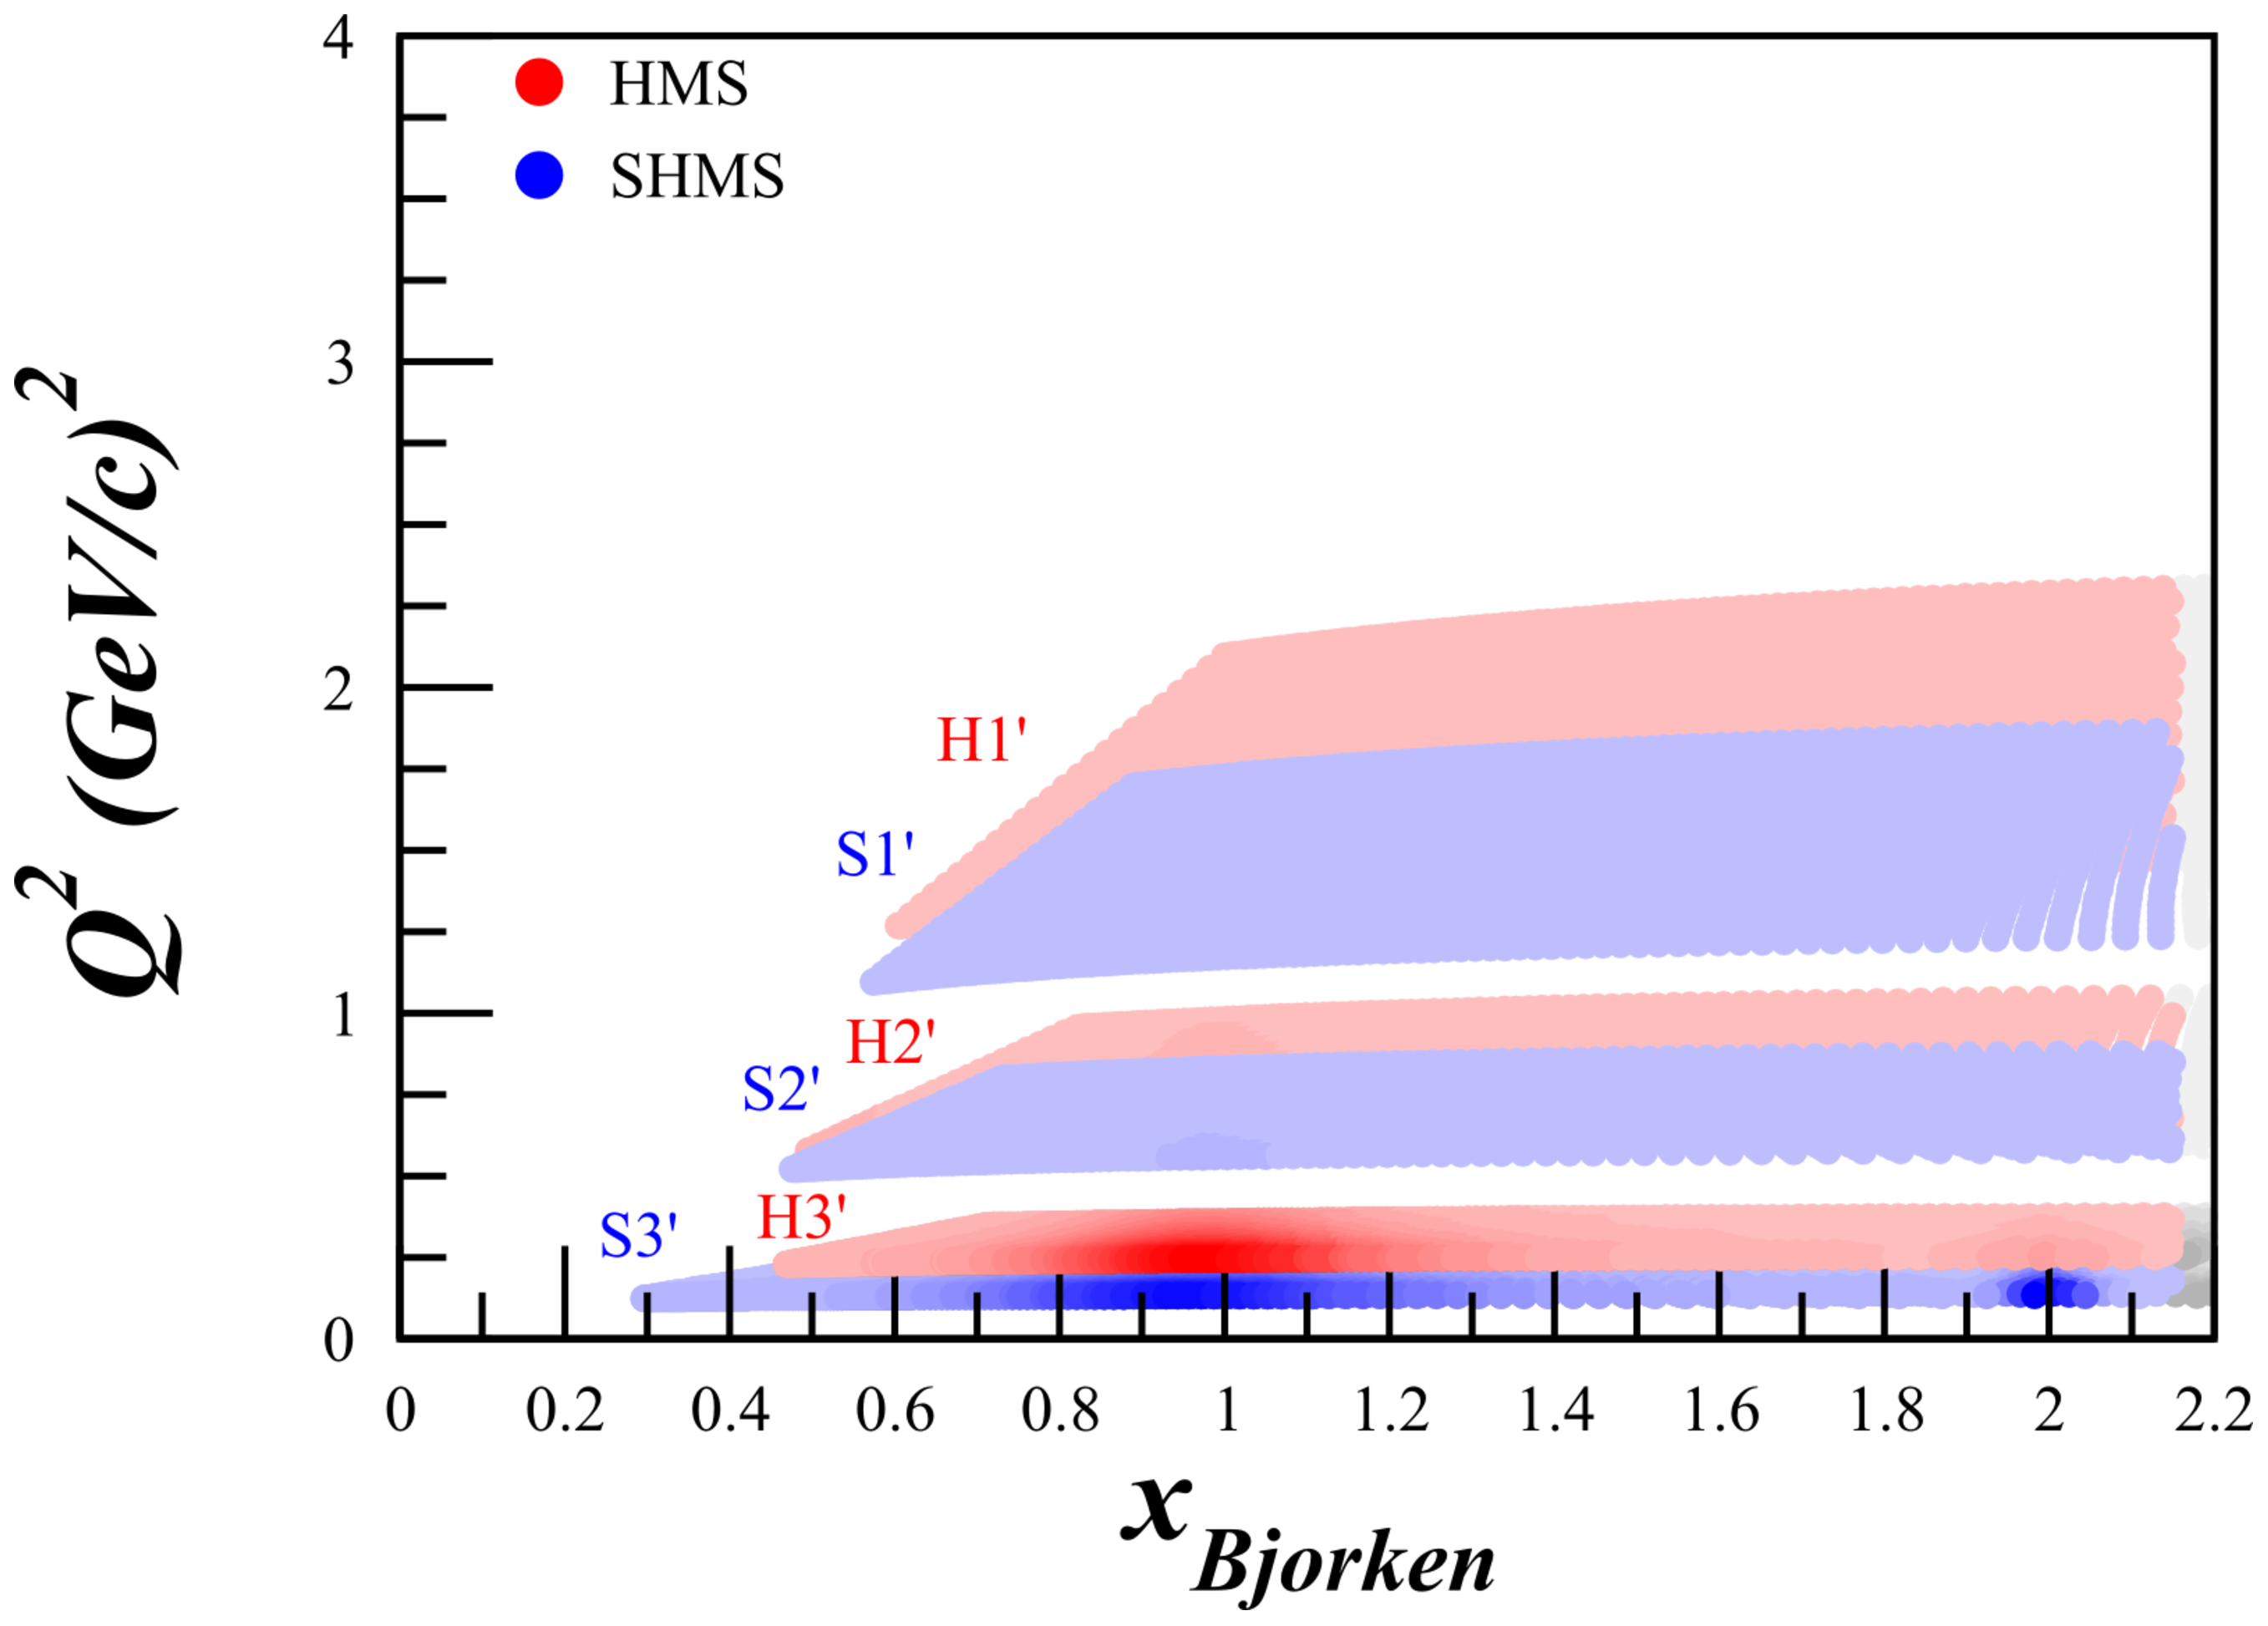
\includegraphics[width=0.49\textwidth]{figs/q2_shms_const.eps}

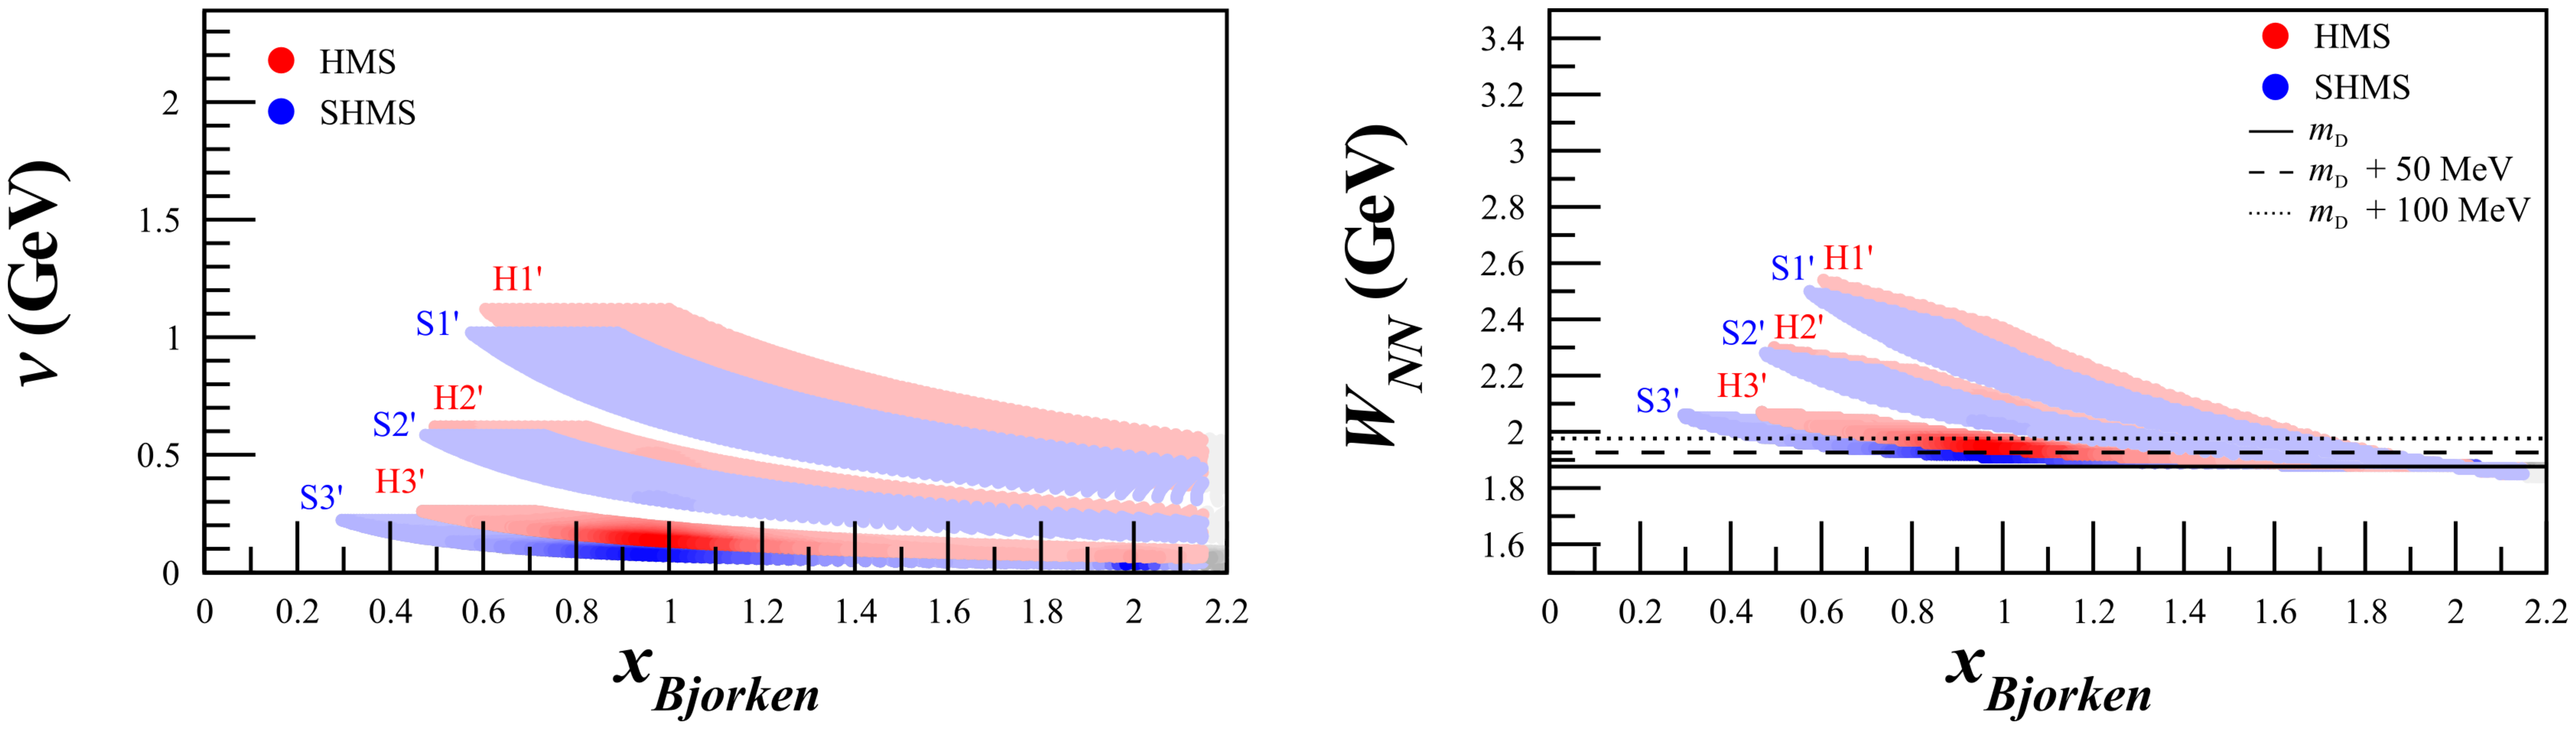
\includegraphics[width=\textwidth]{figs/nu_wnn_shms_const.eps}
%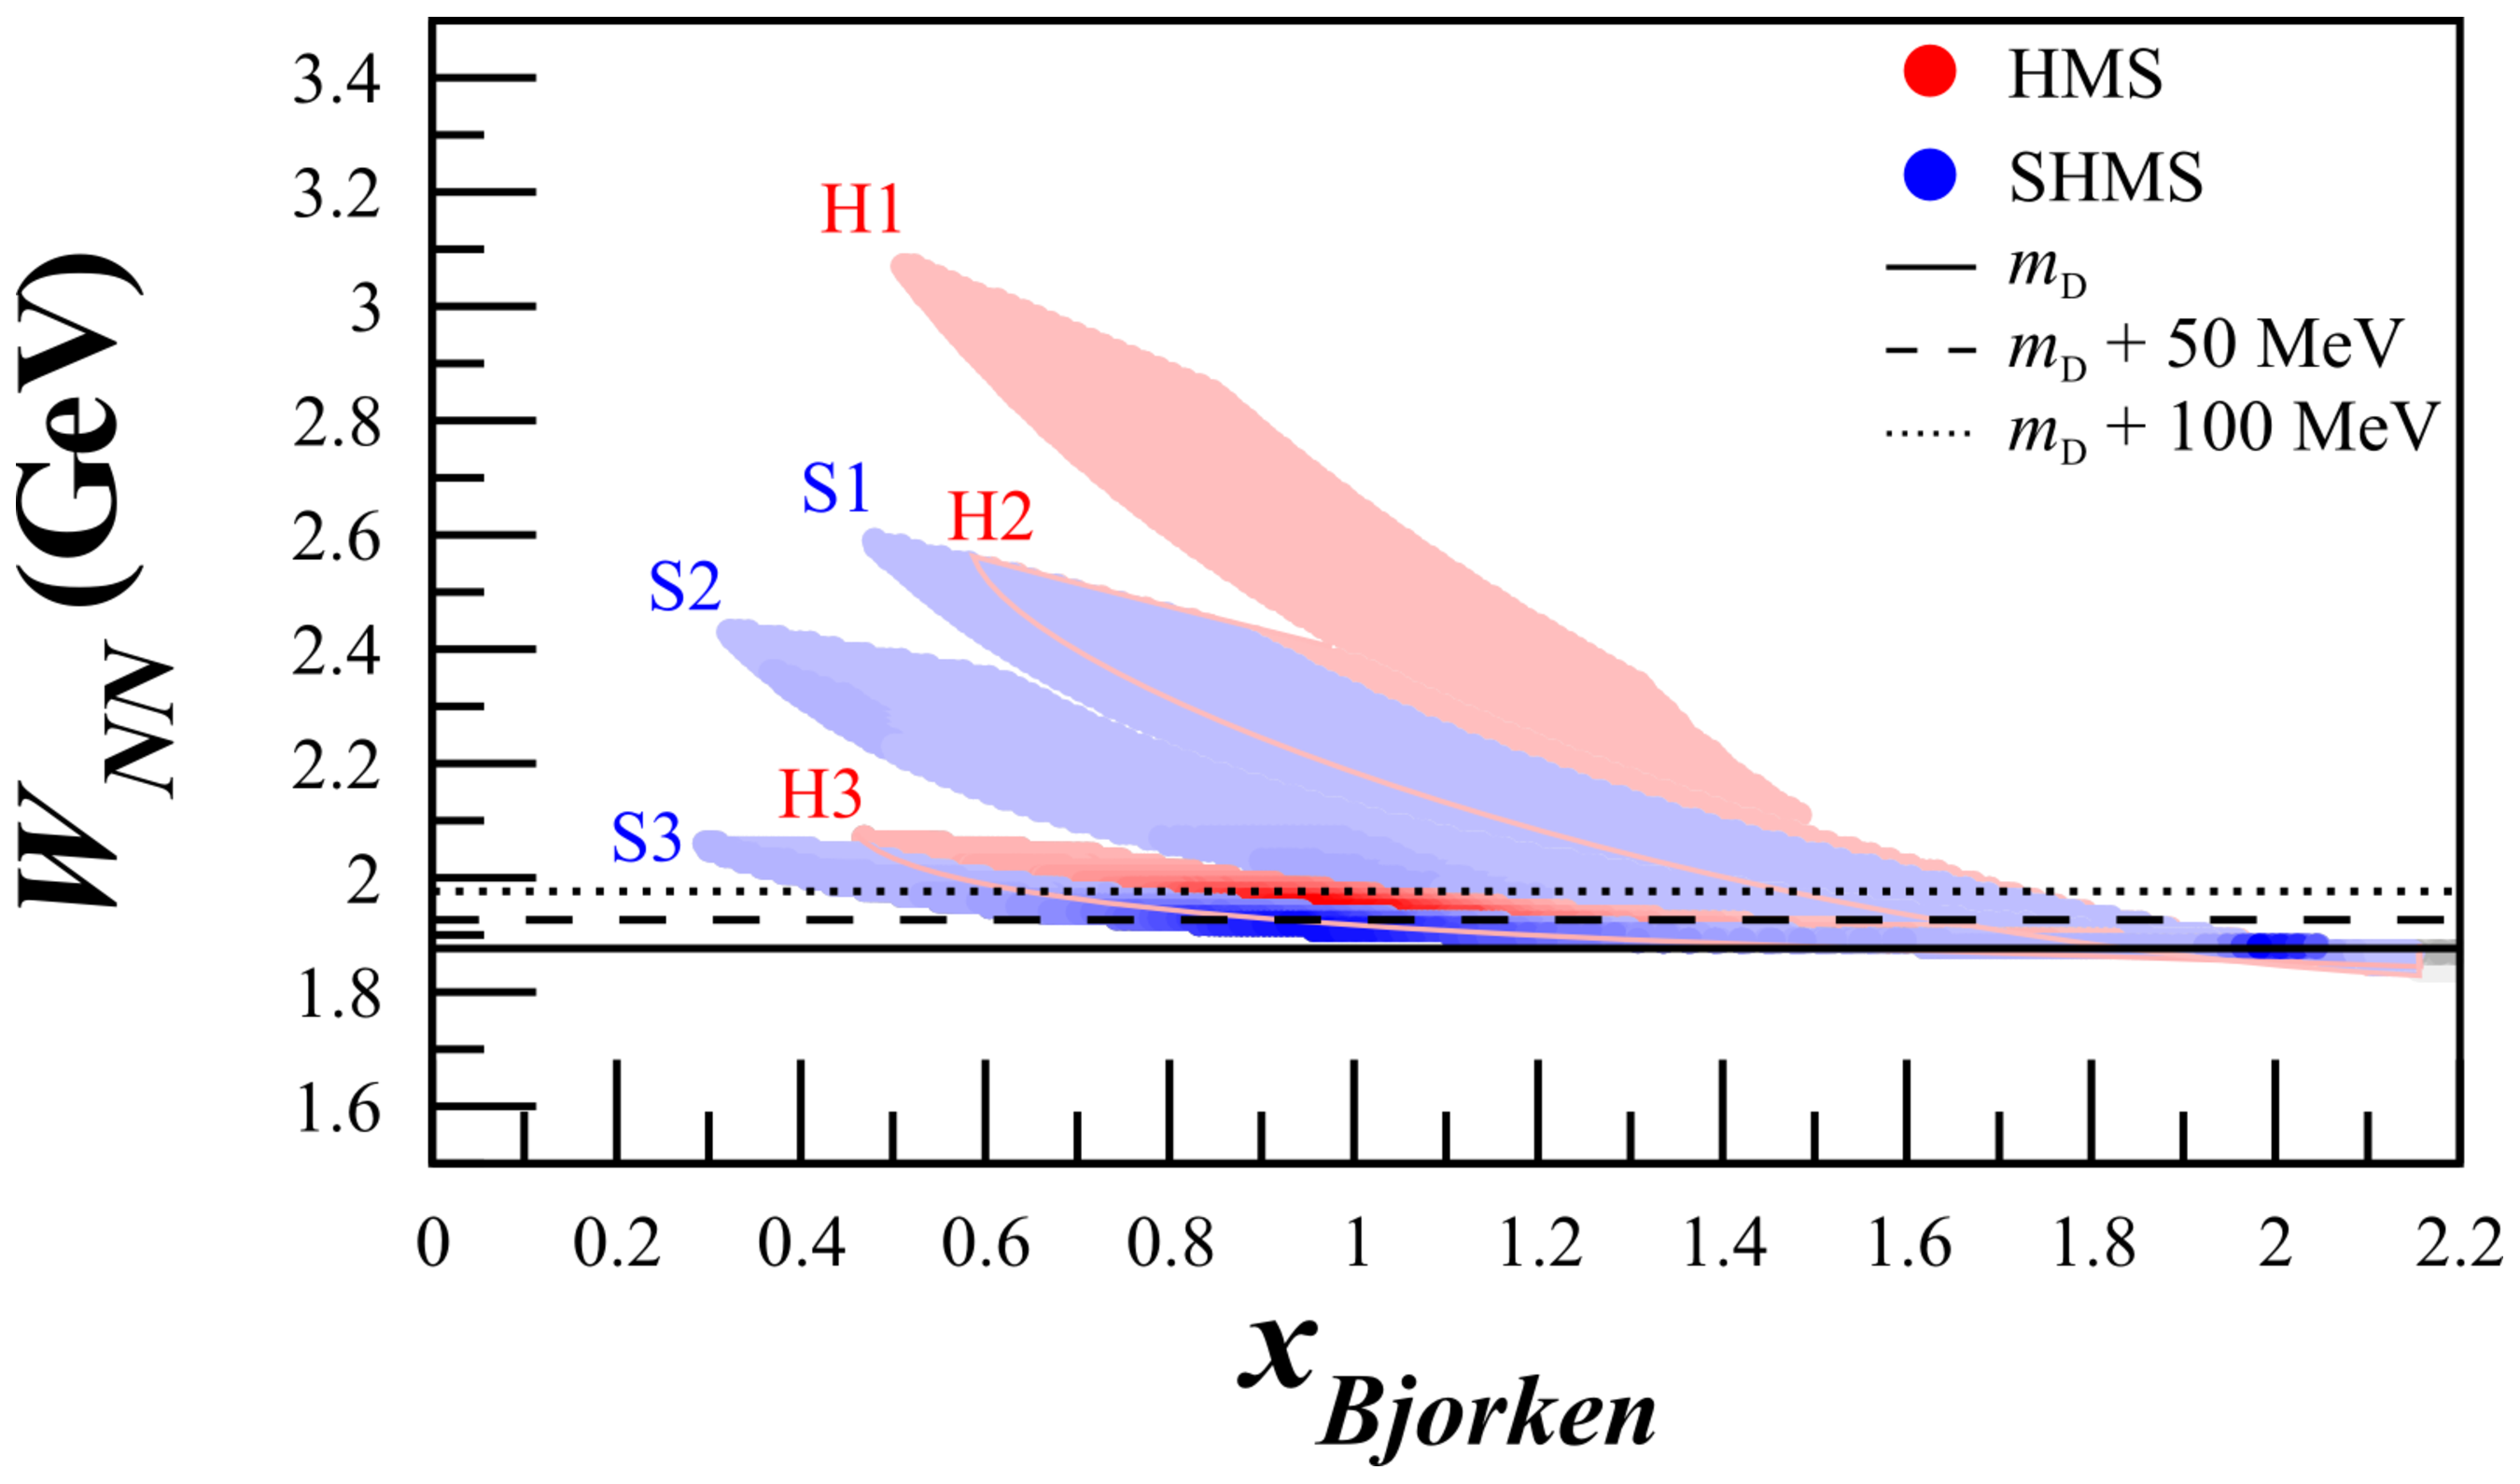
\includegraphics[width=0.49\textwidth]{figs/Pzz_30_all_wnn.eps} %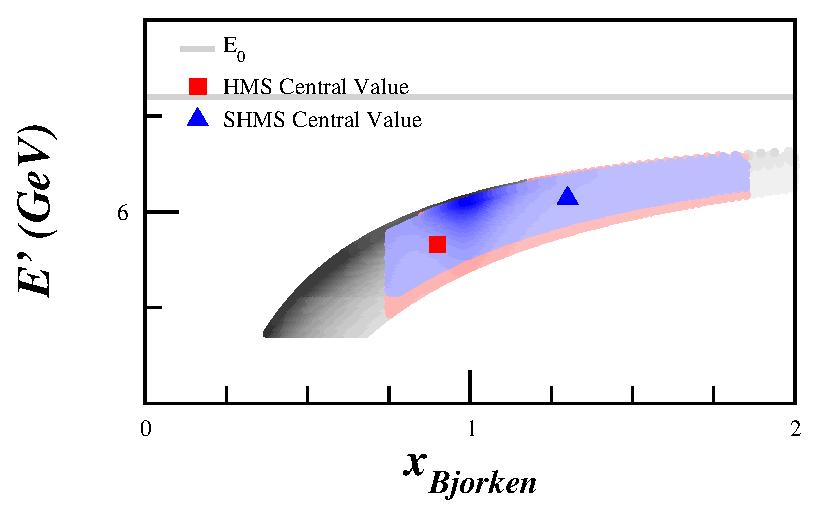
\includegraphics[width=0.49\textwidth]{figs/kine/Pzz_30_eprime.eps}
%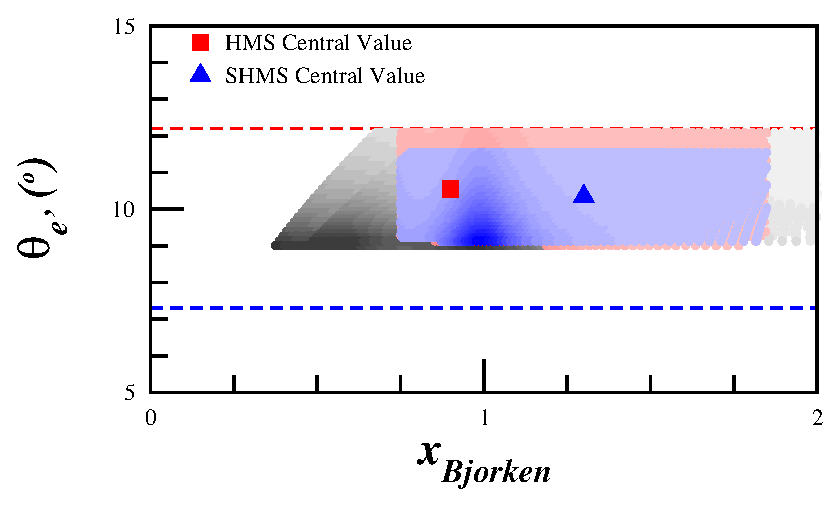
\includegraphics[width=0.49\textwidth]{figs/kine/Pzz_30_theta_eprime.eps}~~ 

\caption{\label{kincov-const} Kinematic coverage for the kinematics listed in Table~\ref{RATES1-const}, which can be achieved in the case that the SHMS is constrained to angles $>10^{\circ}$.}
\end{center}
\end{figure}



\begin{figure}
\begin{center}
\includegraphics[width=0.49\textwidth]{figs/Azz_shms_const.eps} \includegraphics[width=0.49\textwidth]{figs/t20_shms_const.eps} 
\caption{\label{PROJ-const}Projected uncertainties for the tensor asymmetry $A_{zz}$ and elastic analyzing power $T_{20}$ with \productiondays days of beam time using the constrained kinematics in Table~\ref{RATES1-const}.
}
\end{center}
\end{figure}
\fi

\subsection{Uncertainty Estimates}
\label{uncertainties}
We discuss here the expected statistical and systematic uncertainties that we expect to contribute to the measurement.

\subsubsection{Systematic Uncertainty}

%An outline of the systematic uncertainty associated with probing small scale spin-1 tensor asymmetry measurements is presented with some plausible
%approaches to minimize the various contributions.  Some details are specific to a solid state polarized target, others are general instrumental issues.  %Using already approved experiments to collect and study systematic effects can be part of an invaluable program to improve the quality of Hall C data taking.

The spin-1 tensor-polarization dependent observables are part of the family of asymmetries which relies on obtaining data for two different target helicity states under equivalent experimental settings.  A large contribution of the experimental uncertainty that effects absolute normalization cancels out as terms in the denominator and numerator are equivalent.  For situations where the experimental configuration has changed during the data collection of the two different helicity states the cancellation does not occur and a rigorous accounting of the errors is required.

The tensor-polarization dependent asymmetry takes the form
\begin{equation}
A_{zz}=\frac{2}{fP_{zz}}\left(\frac{\sigma_p}{\sigma_u}-1\right),
\label{asy}
\end{equation}
where $\sigma_p$ is the polarized cross section and $\sigma_u$ is the unpolarized cross section. There are of course other spin-1 alignment dependent asymmetries, but for positive quadruple polarization in inclusive scattering all polarized observables can be expressed in terms of $A_{zz}$.

The figure of merit (FOM) for a tensor polarized solid state target can be defined as,
\begin{equation}
FOM=n_tf^2P_{zz}^2
\end{equation}
where $n_t$ is the target thickness and $P_{zz}$ is the tensor polarization.




% \paragraph{Systematic Contributions}
The contributions to the experimental uncertainty come from inaccuracies inherent in the system of measurement of the
observable of interest.  Each experiment contains instrumental components of systematic error which may or may not have
dependence on accessible parameters.  These types of errors can have a nonzero mean that changes over time so that its
effect is not reduced when observations are averaged.  There are also stochastic components to the uncertainty which will vary
only around a single mean.  There may still be a time dependence to the standard deviation of the stochastic contributions
but these types of errors can be reliably estimated by repeating measurements.

Monitoring the systemic coupling of the instrumental parameters can greatly reduce the overall uncertainty produced in small asymmetry measurements. An understanding of the evolution of these types of errors over the course of the experiment can be used to make corrections after data acquisition.  Reducing the time in each target spin orientation can also significantly reduce the impact of shifts in normalization.  However, the stochastic components must be regulated prior to and during the experiment.  Helicity flips can not reduce this type of uncertainty contribution.

Many of the errors that arise from limitations in measurement capacity have a statistical probability distribution that can be accurately estimated. 
For many of these types of uncertainties it is possible to derive confidence limits on the domain of the measured value resulting in a relative
contribution to the total systematic error.  Under an independent error assumption these relative contributions add in quadrature, with polarization
being the dominating uncertainty in the spin dependent observables.  The standard law of combination of errors does not work when there are correlations between these types of uncertainties.  For this situation the full covariance matrix is required and a minimization procedure 
maybe needed to keep the error under control.  This is only relevant for dominant errors.  For multiple kinematic tracking variables strict
estimation and handling of each uncertainty is essential for a complete analysis. In many cases one may wish to assume 100\% correlation between variables to simplify the book keeping for smaller contributions.

Errors are often assumed to have a normal distribution.  In reality measurement errors are rarely distributed
in a true Gaussian and usually have some prominent non-Gaussian tail.  Given a sufficient number of measurements the central limit theorem can
be employed to ensure that the estimated parameters will be more Gaussian than the estimated measurements.

Table~\ref{sys-unc} shows a list of the scale dependent uncertainties contributing to the systematic error in $A_{zz}$.

Polarization error is well understood and steps will be taken to minimize these contributions, as has been done in previous experiments~\cite{keller1}.  There are additional uncertainties that can arise from RF quadrupole polarization enhancement, but recent efforts by the UVA target group to study the tensor-enhanced NMR line-shape indicate that the total uncertainty in this case can be held
under 6\% \cite{keller2,keller3}.

\begin{table}
\begin{center}
\begin{tabular}{l|c|c}\hline\hline
Source                         & $A_{zz}$ Systematic & $T_{20}$ Systematic\\
\hline
Polarization                 &   6.0\%  & 6.0\% \\
Dilution factor              &   6.0\%  & 2.5\% \\
Packing fraction             &   3.0\%  & 3.0\% \\
Trigger/Tracking Eff.        &   1.0\%  & 1.0\% \\
Acceptance                   &   0.5\%  & 0.5\% \\
Charge Determination          &  1.0\%  & 1.0\% \\
Detector resolution and efficiency & 1.0\% & 1.0\% \\
\hline
Total  &  9.2\%  & 7.4\% \\
\hline
\end{tabular}
\caption{\label{sys-unc}Estimates of the scale dependent contributions to the systematic error of $A_{zz}$ and $T_{20}$.}
\end{center}
\end{table}

The dilution factor $f$ varies as a function of scattered electron energy, particularly at
kinematics where nucleon resonances are prominent.  The dilution factor must be known precisely at each kinematic point.  This factor must be based on empirical information with measurable error, which will be measured multiple times at each kinematic setting.  Though the loss to the figure of merit can easily be recovered for lower
$f$, the error calculated from the variation of the models is only a crude estimate.

The other uncertainties in Table~\ref{sys-unc} are very standard contributions which are difficult to reduce beyond the listed instrumental lower limit.

\paragraph{Time Dependent Factors}\mbox{}
\label{timedep}

Eq.~\ref{asy} involves the ratio of counts, which leads to cancellation of several first order systematic effects.  However, the fact that the two data sets will not be taken simultaneously leads to a sensitivity to time dependent variations which will need to be carefully monitored and suppressed when possible.  
%
To investigate the systematic differences in the time dependent components of the
integrated counts, the effects from calibration, efficiency, acceptance,
and luminosity between the two polarization states must be considered.
In order to look at the effect on $A_{zz}$ due to drifts in beam current measurement
calibration and detector efficiency, Eq.~\ref{asy} is rewritten explicitly in terms of the raw measured counts $N_1$ and $N$,
\begin{eqnarray} \label{3c}
\nonumber
A_{zz}&=&\frac{2}{fP_{zz}}\left(\frac{N^c_1}{N^c}-1\right) \\
      &=&\frac{2}{fP_{zz}}\left(\frac{Q\varepsilon l \cal{A}}{Q_1\varepsilon_1 l \cal{A}}\frac{N_1}{N}-1\right)
\end{eqnarray}
where $Q$ represents the accumulated charge, and $\varepsilon$ is the detector efficiency. The target length $l$  and acceptance $\cal{A}$ are identical in both states, to first order.

We can then express $Q_1$ as the change in beam current measurement calibration that occurs in
the time it takes to collect data in one polarization state before switching such that $Q_1=Q(1-\delta{Q})$.
In this notation, $\delta{Q}$ is a dimensionless ratio of charges in the different polarization states.  A similar representation
is used for drifts in detector efficiency leading to,
\begin{equation}
A_{zz}=\frac{2}{fP_{zz}}\left(\frac{N_1Q(1-\delta{Q})\varepsilon(1-\delta\varepsilon)}{NQ\varepsilon}-1\right).
\end{equation}
which leads to,
\begin{equation}
A_{zz}=\frac{2}{fP_{zz}}\left(\frac{N_1}{N}(1-\delta{Q}-\delta\varepsilon+\delta{Q}\delta\varepsilon)-1\right).
\end{equation}

Estimates of $\delta{Q}$ and $\delta\varepsilon$ can be obtained from previous experiments.
For the HRS detector drift during the JLab transversity experiment E06-010, the detector response
was measured such that the normalized yield for the same condition over a three month period indicated little change ($<1$\%).
These measurements indicated that for the short time (20 minutes) between target spin flips,
the detector drift should be less than 1\% times the ratio of the time period between target spin flips and three months.
Also considering the period between target polarization states to be
$\approx$12 hours leading to an overall drift $\delta\varepsilon\sim0.01\%$.  A similar approach can be used to establish an estimate
for $\delta{Q}$ using studies from the g2p/GEp experiment, resulting in $\delta{Q}\sim0.01\%$.  The SANE
experiment with a beam current of 100 nA also provides some information. In this case, the relative stability of the current
monitors is on the order of $1\times10^{-3}$, showing oscillations with a period of about an hour.

Expressing $A_{zz}$ in terms of the estimated experimental drifts in efficiency and current measurement,
\begin{equation}
A_{zz}=\frac{2}{fP_{zz}}\left(\frac{N_1}{N}-1\right)\pm\frac{2}{fP_{zz}}\delta\xi.
\end{equation}
where $\delta\xi=\delta{Q}+\delta\varepsilon$. This leads to a contribution to $A_{zz}$ on the order of $1\times10^{-3}$,
\begin{equation}
dA_{zz}^{drift}=\pm\frac{2}{fP_{zz}}\delta\xi=\pm3.7\times10^{-3}.
\end{equation}

Using the standard dilution factor and classically accessible polarization, the precision required in the raw $A_{zz}$ measurement for already-approved DIS $b_1$ experiment is
\begin{equation}
\delta A_{zz}^{raw}=\frac{fP_{zz}}{2}\delta A_{zz} =1.5\times10^{-4}.
\end{equation}
%The polarization state of the target for $b_1$ will be changed a least every 12 hours, so each of the kinematic settings will involve between $N = 12$ to $N = 60$ polarization cycle pairs.

For this proposed $A_{zz}$ measurement, $f$ is changing with $x$ significantly.  For $x\sim1$ the dilution is
greater ($f\sim0.5$) than for the larger $x$ ($f\sim0.1$), where the large signal size indicated by $A_{zz}$ model calculations requires considerably less precision.
The critical point is $x\sim0.8$ where $f$ is less then $0.2$ such that 
\begin{equation}
\delta A_{zz}^{raw}=\frac{fP_{zz}}{2}\delta A_{zz} =\frac{(0.19)(0.2)}{2}(0.05)=1.0\times10^{-3}.
\end{equation}  
So even this most sensitive point is still around an order of magnitude less constrained than the $b_1$ measurement.

Detector efficiencies can drift for a variety of reasons,
including fluctuations in gas quality, high voltage drift, or
drifts in the spectrometer magnetic fields.  All of these types of variation 
can be controlled and minimized during the experiment through careful monitoring as well as systematic studies of the data collected.  
The identical configuration of the two
polarization states minimizes the relative changes in luminosity with respect to time.  
Consistency checks on the measured cross section data can be implemented to 
ensure the quality of each run used in the asymmetry analysis.
Fluctuations in luminosity due to target density variation can be kept to a
minimum by keeping the material beads at the same temperature for both polarization
states through control of the microwave and the liquid helium (LHe) evaporation.  The helium vapor pressure reading
provides an accuracy of material temperature changes at the level of $\sim$0.1\%.
Beam rastering can also be controlled to a high degree.

The dominant source of any variation in acceptance ${\cal A}$ from state to state will be the stability of the target magnetic field.
The capacity to set and hold the target super conducting magnet
to a desired holding field is $\delta B /B=$0.01\%.  The same target cup will be used
for each state, which removes any variation in the target length $l$. 

\paragraph{Drift Mitigation}\mbox{}

Uncertainty in the measuring devices (or resulting normalization deviations) must be small compared to the
scale of the asymmetry at the helicity reversal frequency.  The beam noise that can contribute to these
normalization deviations comes from beam current, beam position, beam energy, beam size (consistent rastering), and beam halo.  Detectors drifts in photomultiplier tube (PMT) gain can change the number of events above
a discriminator threshold, which can become critical when the device PMT behavior changes significantly between
helicity states.  This is also true for drift chamber efficiency, spectrometer analyzing field,
atmospheric pressure and temperature all affect these systems.
The target's superconducting magnet will be operated in persistent current mode, which provides a field uniformity of better than $10^-4$~\cite{Keith:2003ca}. The NMR resonance frequency can also be used to monitor the field with an accuracy exceeding $10^{-5}$.

%The target holding field stability should never be an issue.%, however in $g_2^p$ this proved not to be the case due to a faulty power supply.  Target field instability could certainly destroy data runs taken with under similar defective circumstances.

The most obvious way to improve the experiment considering these contributions is to increase the helicity flip frequency.
Probably the most practiced way to do this is to use two different target cells alternating the cell position between a
polarized target cell and an unpolarized target cell.  By doing this additional uncertainties from using different packing factions,
effective target densities, and target nuclear-chemical compositions are introduced that would not be present when using identical targets for each helicity state.
These contributions maybe able to be mitigated by alternating which cell is polarized.  It is possible to polarize a particular cell
without being in beam having it outside the homogeneous portion of the target field (beam line).  In this way a target cell helicity can be
prepared while taking data on the other cell.  This could potential allow multiple helicity changes in a 24 hour period.

In addition to greater frequency in helicity changes, the initial polarization build-up
can also be enhanced.  It is possible to install an electrically controlled microwave attenuator which will allow a larger amount of microwave power to dump into the target material to speed up polarization.  The attenuator can then be adjusted to the required power to sustain polarization with the addition of the electron beam.  

The uncertainty estimate in charge that results in a small absolute change in the observable is described
in the proposal in the Section~\ref{timedep}.  Analytically there is a component of uncertainty that propagates with the other
relative errors and only a very small piece that results in a drift in the observable.
The resulting expression for the charge and other contributions to the drift in the observable is expressed as,
\begin{equation}
\delta A^d_{zz}=\pm \frac{2}{fP_{zz}}\delta\xi,
\label{drift}
\end{equation}
where $\delta\xi$ contains the sum of $\delta Q$, $\delta \epsilon$, $\delta l$, and $\delta A$.  This means that
to accurately represent $\delta A^d_{zz}$ we must obtain only the residual deviation from the two polarization
states in the time span of a single cycle (sampling of that data point).  The value used for $\delta Q$ is an estimate based
on the actual effect seen in an observable which helps us to separate the relative contribution from the drift in a given time frame.

\paragraph{Trigger-Tracking}
\label{acc}
For the most part, an easy way to determine whether or not drift will lead to an
effect on the error is to determine if the change over time is seen in one polarization state and not the
other with respect to the observable.  Effects from trigger, cuts, and tracking efficiency do lead to errors in normalization,
however both polarization states see the same stochastic fluctuation over the course of a cycle leading only to a small relative uncertainty in the observable.  Aspects of the error that are non-stochastic
and follow an unknown trend have been estimated in the proposal under the name `detector drifts.'
A secondary estimate was obtained based on HRS detector stability using Hall A transversity data for
detected pions.  The resulting drift was $2.2\times10^{-4}$.
The detector thresholds will be set conservatively while using meticulous on-line monitoring and checks to the relative changes in tracking efficiency between slugs.  For our present estimate including trigger, tracking, cuts, and detector errors that show up strictly as contributions to $\delta\xi$, we estimate no larger than $2.2\times10^{-4}$.

\paragraph{Target Dilution and Length}

There are presently UVA designs for target cup and material fabrication to minimize the probability
of changes to target dilution in the form of material loss over time.  The cup contains
multiple hole arrays that are only a 0.1 mm in size.  The material shape and consistency 
is optimized to maximize the packing fraction and minimize the fracturing capacity.  The
ammonia is hand selected to reduce the structural faults to obtain beads approximately 
2 mm in diameter which have already undergone multiple steps of mechanical stress including being pre-irradiated at NIST with a 10 $\mu$A beam.  The temperature
and thus the density of the target is kept the same
in both polarized and unpolarized states.  There are four temperature sensors in a
standard solid polarized target setup that can be used to monitor this.  The temperature
is controlled via LHe evaporation, microwave, and beam heating.  All three are used
to maintain consistent temperature in both polarization states.

The polarized material to be used in the experiment will be contained in 3 cm 
long, 2.54 cm diameter cylinder cups with their axes parallel to the beam.
The cylinders fit inside the 4 cm diameter vertical cylindrical tail piece at 
the bottom of the refrigerator.  The tail piece is full of liquid helium to 
about 20 cm above the beam level.  The heat and radiation of the beam is distributed
uniformly over the cross section of the target normal to the incident beam by a combination
of slow and fast rasters. The fast raster normally is a 2mm by 2mm square shape, traced by the 
sub-millimeter beam at kHz rates.  The slow raster normally is a 1 cm maximum radius spiral, traced at constant tangential speed, covering the rastered area with 5\% dose uniformity at 30 Hz
and can be synchronized to the usual helicity flip signals \cite{chenyan}.

The averaging of the target length done by the rasters results in an effective 
length that is determined by the fraction of the cup volume 
(equivalently, the rastered volume) that is filled with ammonia \cite{chenyan}.
A possible change in the effective target length between the polarized and 
unpolarized periods of a measurement cycle could come from a net change of 
material in the raster volume. Since the raster diameter is 25\% smaller than 
the cup diameter, there is always material outside the raster region that would
fill in an unlikely loss in the rastered region.
A possible estimate of the length change can be obtained by considering the 
ratio of the 0.008 cm$^3$ volume of a fragment to the 6.8 cm$^3$ raster volume 
(including packing fraction) the ratio is $\sim 1/850$.

The only documented instance with ammonia polarized targets and CEBAF $\sim$ 100 
nA beams of a possible rearrangement of material about the target NMR coil that
might indicate an associated net change in material was seen during E07-003 (SANE) which took about 500 hours of $\ge$ 85 nA beam. 
During one 20 h polarized and unpolarized cycle, the loss of 1 or 2 fragments 
would result in a $\sim 1\times 10^{-3}$  change in target length, with a 
$\sim$ 20h/500h probability.
No instances of material fragmentation, which could potentially lead to net 
losses in the raster region have been observed with up to 150 nA CW CEBAF beams 
(E93-026, E01-006, E07-003).  In addition, there are checks in NMR data that can be
used to ensure that no loss of a target fragments occurred between cycles. 

The only instances of material fragmentation for ammonia targets were observed 
at SLAC, in the E143/E155/E155x series of experiments, but the SLAC beam is 
pulsed, with 4 $\mu$s wide pulses of $\sim$20 $\mu$A current at 120 Hz repetition
rate. Such beam time structure can be expected to damage the ammonia crystals by
thermal shock. In fact, to further prevent possible shock effects at JLab, the 
polarized target experiments in Hall C implemented the procedure of gradual
ramping up of the beam current after beam trips.

All changes to the material that occur during movement of the target ladder or
annealing can only happen at the end of each pair of measurement cycles and are
irrelevant for the preceding or following cycles.  Small changes to material
NMR loop coupling are consistent to both polarization states and exist as
a relative error in the polarization.
In addition, as long as the LHe is superfluid ($<2$ K),
its flow can not lead to material rearrangements.  The LHe that is fed
at the bottom of the nose piece coming from the separator is below 2~K, so emptying 
and refilling does not have any effect.

Depolarization using LHe is a relatively standard technique.  In this procedure, the
beam is turned off and the LHe fill valve that controls the
LHe level that surrounds the target insert is slowly reduced as to not replenish
the LHe evaporation until the material has warmed up and the polarization has died out.
The LHe is gradually filled again as in the standard evaporation mode and again set on
automated control.  Once the material is unpolarized and again submerged under
the LHe the microwaves are turned on in off-resonance mode.  The unpolarized target
is then ready for beam.  This procedure provides a quick way to kill polarization while
returning the unpolarized state to the exact condition of the polarized state.  The
small fluctuation in density, temperature and NMR material couple occur in both states
and are a small relative error in the polarization.  All other aspects that may result
in addition to the drift are negligible. 

For example, the target operating temperature is $\sim 1.1\pm 0.15$ K, well below the 
superfluid point.  Over that range, the LHe density, changes by $4\times
10^{-5}$ (the density actually increases below $\simeq 1.1$~K
and increases above, by about equal amounts over the temperature 
interval~\cite{lhe}).
The lattice constant of deuteroammonia~\cite{nd3} changes from 5.048~\AA\ at 2~K to 5.073~\AA\ at 77~K, corresponding to a $1\times 10^{-5}$ change over the 
$\pm$0.15~K interval considered above.  For a 60\% packing fraction, the change 
would be $2.3\times10^{-5}$ for a 0.15~K unexpected temperature difference between
polarization states.
Any possible unaccounted changes in target length between the polarized and 
unpolarized parts of each cycle can also be monitored by recording the time 
dependence of the luminosity with a $\simeq 0.5\times 10^{-4}$ accuracy. %It's our understanding that such device is available in the Hall.

\paragraph{Solid Angle}\mbox{}

The error that arises in the observable due to beam position and magnet currents
over time is inherently very difficult to separate into drift and relative uncertainty.
The 0.1\% error over a 12 hour period is probably quite accurate, however, being
that both polarization states experience the same fluctuations its likely that the majority
of the uncertainty is relative.  There are also concerns on acceptance due to beam position drift. Beam drift
will be monitored during the experiment and accounted for during analysis.  The largest part of this
uncertainty is also a relative contribution to both target states.  The contribution to the drift can be minimized
with the feedback system built for parity experiments
%, which is discussed further in Section~\ref{regress}
.

Trends that arise from dependence of yield on
magnet currents in detectors are a concern related to the spectrometer acceptance.  The drift
effect can be made to be small, for the HRS typically less than $10^{-4}$ for the dipole
and $10^{-3}$ for the three quads, and similarly for the HMS.  The effects on the acceptance can be determined and
corrected through careful analysis.  Naturally, the
target magnet current does not need to be changed between cycles, as the uniformity, stability, and setability
pointed out in the proposal eliminate field variation between the two polarization
states.  The residual drift from solid angle effects after such correction is expected to be no larger than 0.01\%.
This value was already accounted for in Section \ref{acc}.

\iffalse
\paragraph{Multivariate Regression}\mbox{}
\label{regress}

The error that arises in the observable due to drifts in beam current or position, analyzing magnet currents,
and many others can depend on many parameters that may be available such as instrument temperature, gas levels in spectrometer,
ambient conditions in the Hall, etc.  This type of information can be made part of the data stream and can be used in a regression
analysis to understand the change in the normalization components between the different helicity states.  A correction can then
be made mitigating the false asymmetry from that specific deviation.
\begin{figure}
\begin{center}
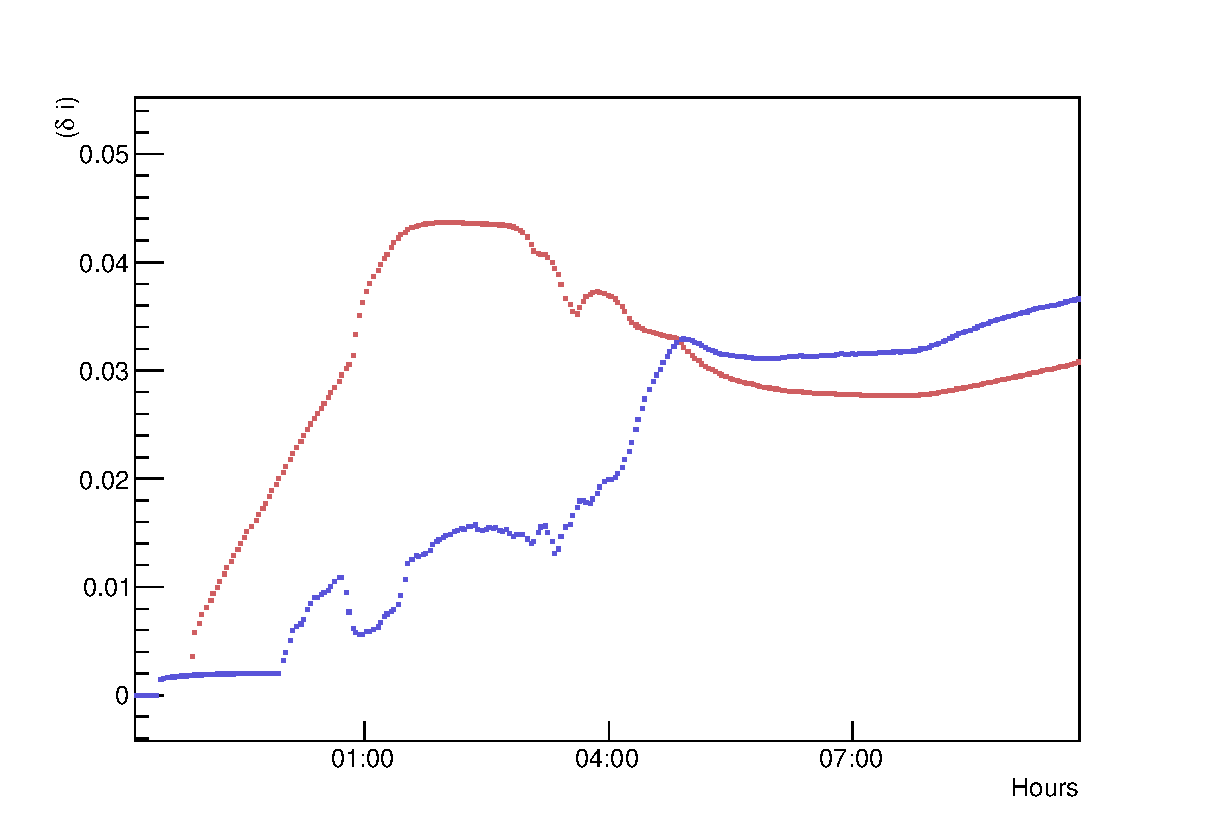
\includegraphics[height=75mm, angle=0]{./figs/dev}
\end{center}
\caption{Hypothetical deviation of the two Hall C beam current monitors.}
\label{dev}
\end{figure}
Figure \ref{dev} show a hypothetical deviation of the two Hall C BCM.  The $y$-axis is the current percent deviation in a BCM affected by temperature changes
evolving in time.  This is for a demonstration only and is a simulation based on
data taken from previous experiments.  The simulation incorporates a systemic coupling
to temperature which could be reconstructed using a multivariate regression.

Figure \ref{qweak} shows the ratio of the two standard Hall C beam current monitors over a 40 hour period during the Q-weak experiment.  The
variation in the two beam current monitors is thought to have a strong dependence on monitor unit temperature.  Having a measurement of temperature of each
monitor over time gives additional information that can be used to model the dynamic behavior of the beam current deviations.  

\begin{figure}
\begin{center}
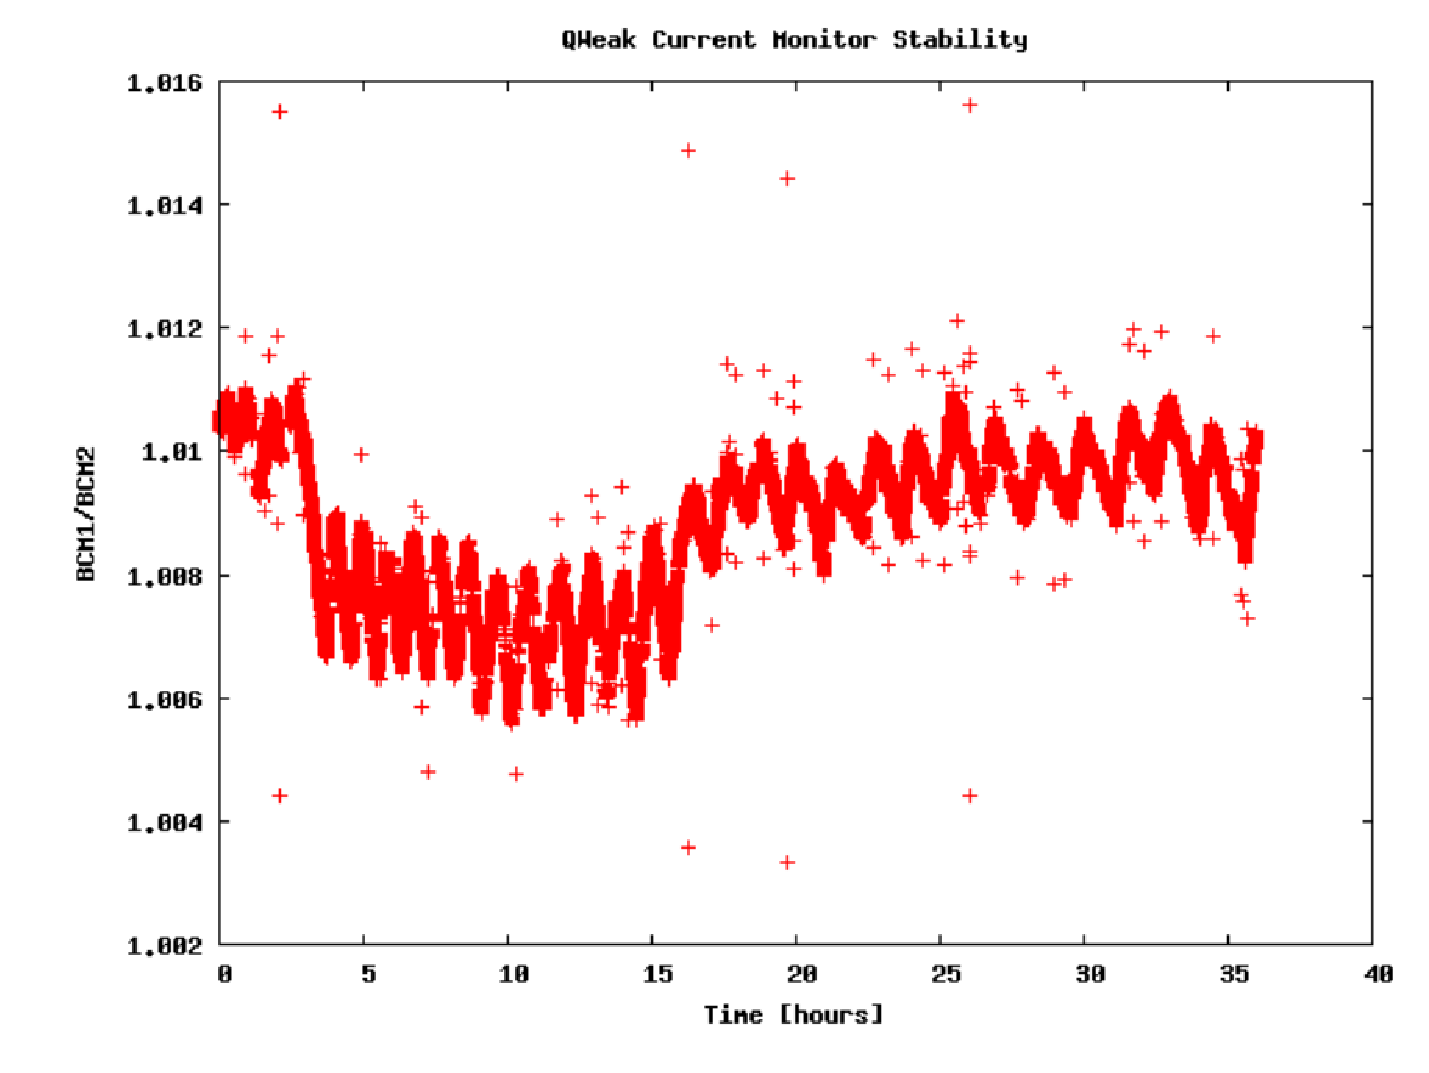
\includegraphics[height=75mm, angle=0]{./figs/qweak}
\end{center}
\caption{The ratio of the two standard Hall C beam current monitors over a 40 hour period during the Qweak experiment.}
\label{qweak}
\end{figure}

To use an example with real data, consider the polarization normalization changes as a function of the Q-meter.  There are linear scaling effects that
lead to a shift in the DC-offset as well as nonlinear contributions that effect the systems capacity to measure accurately.  These effects are a function
of both time and temperature.  A simple regression using a linear model is used based on the deviation seen in polarization at different temperature, as shown in Fig. \ref{PolTemp}.
The model can be used to correct the polarization given any temperature of the Q-meter NMR.  The nonlinear effects are not seen as a function of temperature as much as a
function of time.  This is likely because certain parts of the circuit heat up at different rates having separate but correlated effects.  The basic linear model can be
improved by simply adding the time-stamp into the data-stream and running a multivariate analysis using polarization, time and temperature.  Figure \ref{regression} show
four different trials using a Artificial Neural Network and well as a Boosted Decision Tree.  The $y$-axis shows $g(T)$ average deviation (with error bar showing the spread of deviation) from the true value and the measured/correct value.  From the left each point reflects no correction, linear model correction, multivariate regression using temperature, and multivariate regression using temperature and time, respectively, as part of the feature space. 
\begin{figure}
\begin{center}
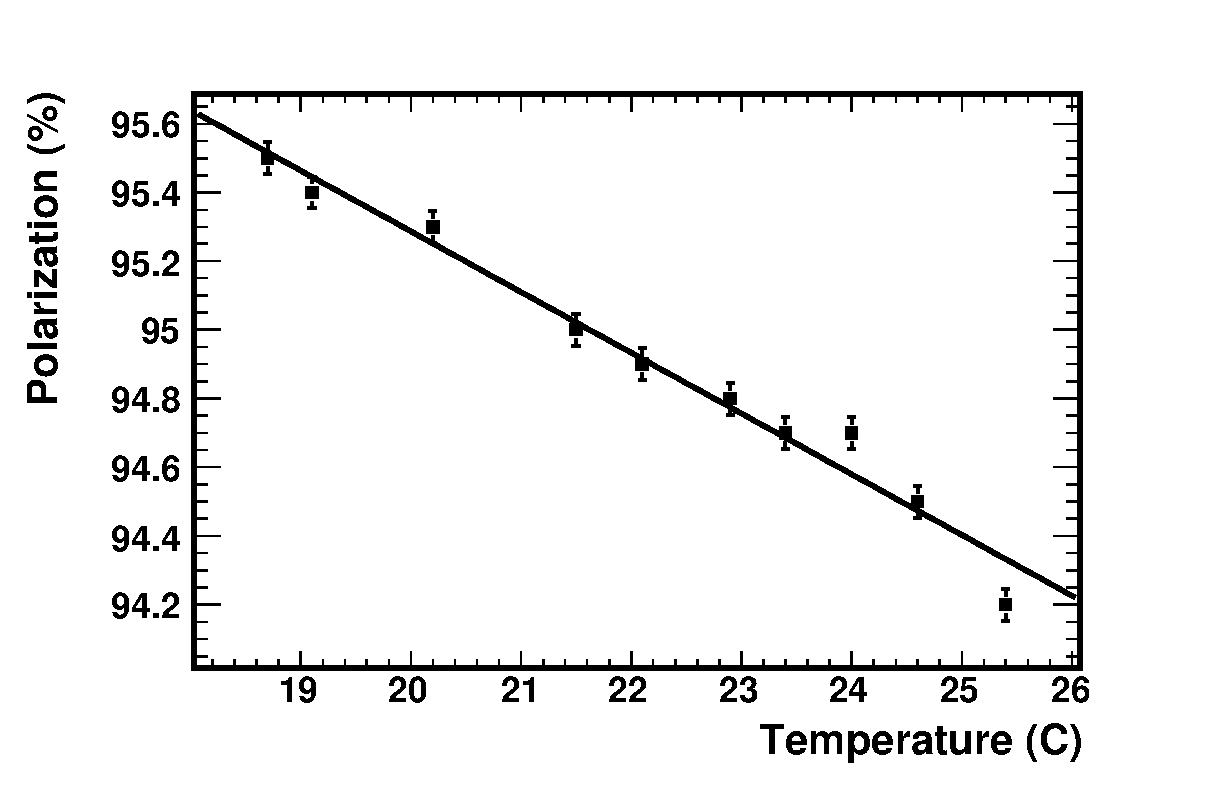
\includegraphics[height=75mm, angle=0]{./figs/PolTemp}
\end{center}
\caption{A simple regression using a linear model is used based on the deviation seen in polarization at different temperature}
\label{PolTemp}
\end{figure}

It is possible to measure the change in an element of drift with respect to other parameters.  Measurements of this systemic coupling
can be used to disentangle effects that are driven by changes in the environment over time.  For example, knowledge of luminosity monitors or BCM temperature
can be used in regression to account for changes in the values.  Drifts that change as a function of some quantifiable parameter can be understood
and corrected if that parameter is also recorded in time.  This type of empirical information taken over several experiments can be invaluable 
for the experiments to follow.  This is exceedingly true with the use of multivariate regression where multiple variables over multiple experiments can be used to train a learning algorithm to interpret various environmental contributions and deduce the effects on essential covariance trends.  %More research would be needed to implement these techniques in the modern experimental hall infrastructure.

\begin{figure}
\begin{center}
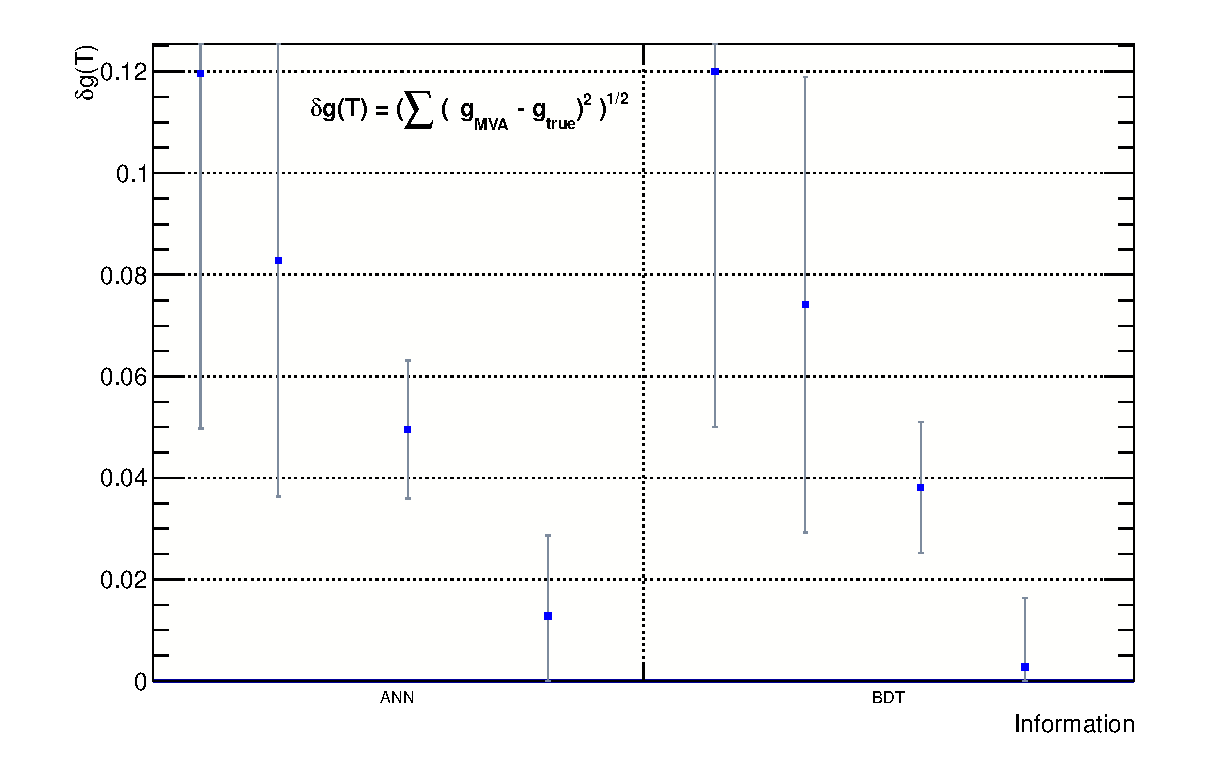
\includegraphics[height=75mm, angle=0]{./figs/Regression}
\end{center}
\caption{Average deviation for the (from left) no correction, linear model correction, multivariate regression using temperature, and multivariate regression using temperature and time as part of the feature space.  The left (right) plot uses an Artificial Neural Network (Boosted Decision Tree) as the multivariate algorithm.}
\label{regression}
\end{figure}
\fi


\paragraph{Beam Current Monitors}\mbox{}

Information has been extracted from experiment E06-010 for high current (10-15 $\mu$A),
in which all the systematics are included in the yield studies including detector
drift, acceptance drift, BCM drift and acceptance due to BPM drift.
The beam charge asymmetries between two helicity states using the luminosity monitors for experiment E06-010 has been shown to be at the level of $4\times10^{-5}$ with a width of $2.3\times10^{-4}$.  An additional estimate on the change in the BCM calibration
constant is seen in experiment E08-027 resulting in a absolute deviation of $2.0\times10^{-4}$ over the course
of six days.  Long term drifts can be reduced by careful thermal isolation of the BCMs, however resulting trends will be need to be studied and corrections implemented.  
%It should be considered a priority to monitor and correct for remaining temperature dependence.

Fluctuations in the calibration of beam current measuring devices can be well understood
and mitigated.  Even when calibrations are taken frequently, a small change in the BCM response over
the course of a single helicity flip iteration can contribute a drift on the order of $1\times10^{-4}$.
%As mentioned previously,
A Boosted Decision Tree regression maybe used similar to that used for the temperature dependence
of the Q-meter.  This would require accurate temperature monitoring of the BCM stainless steel pillbox
resonant cavity in operation.  Creating a heat regulating system using a fluid circulated chiller could
help to both stabilize and accurately measure the temperature.  Additional temperature stabilization of analog cables, and optimizing cable length maybe also help.


\iffalse
\paragraph{Multivariate Dilution Factor}
The change in dilution as a function of $x$ must be known very well.  The uncertainty based
on the variation in models is likely to be grossly underestimated.  If not, and the models
accurately reflect the change in dilution around the $x \approx 1$ and resonance regions, it maybe
possible to extract a near background free set of counts reducing the effective dilution
that goes into the asymmetry calculation.  Using a reliable model or direct empirical information
it is possible to train a Boosted Decision Tree (BDT) to discriminate between the different various
contributions to the spectrum.  Though it is for a two arm experiment, this type of procedure was
suggested for the UVA real Compton scattering experiment (RCS) \cite{Day}.  Using only one arm implies a
great reliance on the model of the dilution, which will likely always be a weak point in this
experiment even with the application of advance techniques.  It is unclear how well this could
work for $A_{zz}$ but I can mention some highlights from RCS.

For the real Compton initial state helicity correlations asymmetry, a photon and proton are detected.
It is not trivial to obtain data free of background events. However, it is possible to obtain
data free of signal events, by selecting different regions of the $\delta X$ and $\delta Y$ phase
space, so that accurate numbers can be obtained for the asymmetry of
pion events. It is then possible to measure the asymmetry for pure background events, the asymmetry for mixed
RCS-background events, and the fraction of the latter events that are RCS.  The latter number is
has a direct effect on the dilution factor in the polarized asymmetry calculation.
Each step can contribute to the error in the resulting RCS asymmetry on both a systematic 
and statistical level.  To consider a technique of
directly extracting the real Compton events negating the need for the asymmetry for mixed
RCS-background events a Monte Carlo simulation is used.  The RCS single events and $\pi^0$ background
events are generated and used to train the multivariate algorithm. 

The result of analysis from the training
of the boosted decision tree indicating the response of the classifier is shown in the left plot.
The real Compton signal resolving efficiency as a function of the cut on the BDT response can be understood using
multiple iterations of the Monte Carlo along with Signal efficiency and background efficiency.  The optimal cut is determined by
using the derivative of the significance function $S/\sqrt{S+B}$.
The classifier response indicated that even with the only three mentioned
discriminating variable it is possible to obtain greater then 98\% signal
when making a constraint on the BDT response to eliminate the pion
background.  The separation using a Monte Carlo demonstration is shown in Fig.~\ref{fig:d11}  
\begin{figure}[h]
\begin{center}
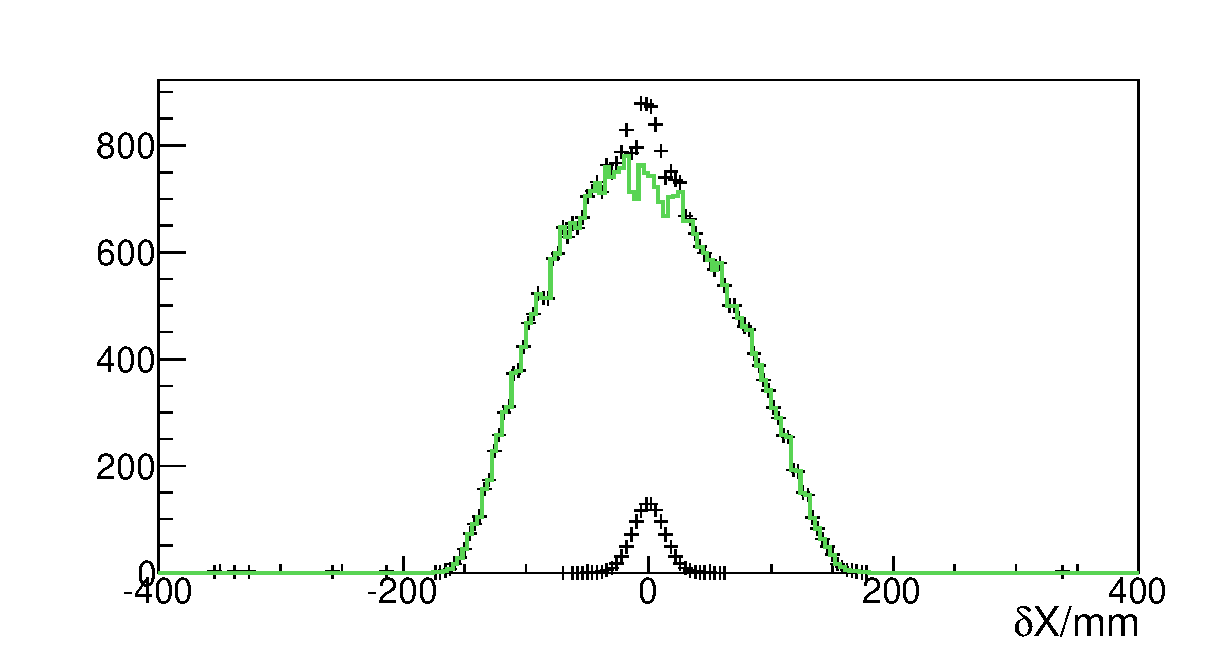
\includegraphics[height=75mm, angle=0]{./figs/d11}
\caption{The $\delta X$ distribution with signal and background before separation and after.
The result of imposing the optimal BDT response cut at 0.063 leading to a RCS event extraction
with 98\% signal efficiency.  This demonstrates a separation with 1000 Compton events and 10000 $\pi^0$ background events.
This is only a Monte Carlo demonstration.}
\label{fig:d11}
\end{center}
\end{figure}

This technique is especially useful for situations in which the background
is difficult to distinguish from the signal in the spectra.  Through the use of multivariate
discrimination of the phase space even a small signal that is nearly
unrecognizable among the background can be separated out with a well defined
uncertainty associated with it.
\fi

\paragraph{Systematic Summary}\mbox{}


It is essential to consider each uncertainty and each source separately as well as understand systemic coupling.  
This proposed $A_{zz}$ measurement would be a great benefit to understand and minimize systematic uncertainties for small asymmetry measurements such as $b_1$. Having data at a large range of beam
current, energy, and target types while studying beam noise and detector stability can help to build a comprehensive map of critical systematic issues. Other systematic minimization techniques can be explored during $A_{zz}$ in addition to the systematic minimization mentioned in this proposal, which will be critical for $b_1$~\cite{Keller:2015tn} and could help many other future experiments. In fact there is no better experimental opportunity to study the systematics of probing asymmetries in Hall C then $A_{zz}$ at high $x$. Because of the scale of the predicted asymmetry $A_{zz}$ for large $x$, the drifts that can corrupt
$b_1$ are only relevant for the lower $x$ points, although for $A_{zz}$ in this region a systematic error of the order of ($1\times10^{-3}$) would be very good, which has an order of magnitude more leeway
then for $b_1$. 



\iffalse
\subsubsection{Systematic Uncertainty}% in $A_{zz}$ }
\begin{table}
\begin{center}
\begin{tabular}{l|c}\hline\hline
Source								& Systematic \\
\hline
$P_{zz}$ Polarimetry					& 12\%   \\
Dilution Factor						& 6.0\%   \\
Packing Fraction						& 3.0\%   \\
Trigger/Tracking Efficiency			& 1.0\% \\
Acceptance							& 0.5\% \\
Charge Determination					& 1.0\%  \\
Detector Resolution and Efficiency	& 1.0\% \\
\hline
Total								& 14\%   \\
\hline
\end{tabular}
\caption{\label{error1}Estimates of the scale dependent contributions to the systematic error of $A_{zz}$.}
\end{center}
\end{table}

Table \ref{error1} shows a list of the scale dependent uncertainties contributing to the systematic error in $A_{zz}$.
With careful uncertainty minimization in polarization the relative error in vector polarization, $Pz$, can be less than or equal to 3.9\%, as was demonstrated for the proton in the recent E08-027/E08-007 experiment~\cite{NIMDUST} and nearly as good for the deuteron using multiple techniques to measure the NMR signal as discussed in ~\cite{PTSTDUST}.  With the use of a positive tensor enhanced target it has been projected to be able to achieve a relative error in $P_{zz}$ better than 12\% ~\cite{PTSTDUST}.  The uncertainty from the dilution in the polarized target is estimated to be
about 6\% over the range of kinematics points of interest.  We consider separately the uncertainty in the packing fraction of the ammonia target contributes at a level of less than 3\%. Charge calibration and detector efficiencies are expected to be known better to 1\%. 
%but the impact of time-dependent drifts in these quantities must be carefully controlled.

\subsubsection*{Time Dependent Systematic Effects}
Eq.~\ref{3} involves the ratio of counts, which leads to cancellation of several first order systematic effects.  However, the fact that the two data sets will not be taken simultaneously leads to a sensitivity to time dependent variations which will be monitored and suppressed. The typical size of these types of effects are small compared to the large asymmetries predicted for most of the proposed kinematic regions, but must be carefully monitored whenever the expected asymmetry is small, such as at a zero crossing.

%While typical false asymmetries in Hall C of $0.1\%$ are acceptable for this proposed measurement, we are interested in a strict control of the systematics for further reduction.
%
To investigate the systematic differences in the time dependent components of the integrated counts, we need to consider the effects from calibration, efficiency, acceptance, and luminosity between the two polarization states.

Fluctuations in luminosity due to target density variation can easily be kept to a minimum by keeping the material beads at the same temperature for both polarization states by control of the microwave and the LHe evaporation.  The He vapor pressure reading gives accuracy of material temperature changes at the level of $\pm0.1\%$.
%Beam rastering can also be controlled to a high degree.

The beam charge asymmetries between two helicity states using the luminosity monitors for experiment
E06-010 has been shown to be at the level of $4 \times 10^{-5}$ with a width of $2 \times 10^{-4}$.
An additional estimate on the change in the BCM calibration constant is seen in
experiment E08-027 resulting in a absolute deviation of $2 \times 10^{-4}$ over the course of six
days. We expect to be able to minimize long term drifts by careful thermal isolation of
the BCMs.
%, however resulting trends will be studied and corrections implemented.

The acceptance of each cup can only change as a function of time if the magnetic field changes.  
The capacity to set, reset, and hold the target superconducting magnet to a desired holding field causes a field uncertainty of $\delta B /B=0.01\%$. 
This implies that, like the cup length $l$, the acceptance ${\cal A}$ for each polarization state is the same.

In order to look at the effect on $A_{zz}$ due to drifts in beam current monitor calibration and detector efficiency, we rewrite Eq.~\ref{3} explicitly in terms of the raw measured counts $N_p^c$ and $N_u^c$,
\begin{eqnarray} \label{3c}
\nonumber
A_{zz}&=&\frac{2}{fP_{zz}}\left(\frac{N^c_p}{N^c_u}-1\right) \\
      &=&\frac{2}{fP_{zz}}\left(\frac{Q\varepsilon l \cal{A}}{Q_1\varepsilon_1 l \cal{A}}\frac{N_p}{N_u}-1\right)
\end{eqnarray}
where $Q$ represents the accumulated charge, and $\varepsilon$ is the detector efficiency. The target length $l$ and acceptance $\cal{A}$ are identical in both states to first order.

We can then express $Q_1$ as the change in beam current measurement calibration that occurs in
the time it takes to collect data in one polarization state before switching to another, such that $Q_1=Q(1-dQ)$.
In this notation, $dQ$ is a dimensionless ratio of changes in different polarization states and would ideally be equal to zero.  A similar representation
is used for drifts in detector efficiency leading to,
\begin{equation}
A_{zz}=\frac{2}{fP_{zz}}\left(\frac{N_pQ(1-dQ)\varepsilon(1-d\varepsilon)}{N_u Q\varepsilon}-1\right).
\end{equation}
which simplifies to,
\begin{equation}
A_{zz}=\frac{2}{fP_{zz}}\left(\frac{N_p}{N_u}(1-dQ-d\varepsilon+dQd\varepsilon)-1\right).
\end{equation}

We obtain estimates of $dQ$ and $d\varepsilon$ from previous experimental
studies.  During the JLab transversity experiment E06-010, the detector drift was measured such that the normalized yield over a three month period indicated little change ($<1$\%).
These measurement were then used to show that for short time (20 minutes periods between target spin flip),
the detector drift was estimated to be less than 1\% times the ratio of the time period between target spin flip and three months.
For the present experiment we use the same estimate except for the period between target polarization states used is
$\approx 36$ hours leading to an overall drift $d\varepsilon\approx 0.01\%$.  A similar approach is used to establish an estimate
for $dQ$ using studies from the data from the E08-027 experiment resulting in $d\varepsilon \approx 0.01\%$.

To express $A_{zz}$ in terms of the estimated experimental drifts in efficiency and current measurement we can write,
\begin{equation}
A_{zz}=\frac{2}{fP_{zz}}\left(\frac{N_1}{N}-1\right)\pm\frac{2}{fP_{zz}}d\xi.
\end{equation}
This leads to a contribution to $A_{zz}$ on the order of $1\times10^{-3}$,
\begin{equation}
dA_{zz}^{drift}=\pm\frac{2}{fP_{zz}}d\xi=\pm3.7\times10^{-3}.
\end{equation}
%For this estimate we assume only two polarization state changes in a day. If it is possible to increase this rate then the systematic effect in $A_{zz}$ will decrease accordingly.

Naturally detector efficiency can drift for a variety of reasons, for
example including fluctuations in gas quality, HV drift or
drifts in the spectrometers magnetic field.  All of these types of variation as can be realized both
during the experiment though monitoring as well as systematic studies of the data collected.
Checks on the consistency of the cross section data that can be use ensuring the quality of each run will be used in the asymmetry analysis.  Regression can be use to correct for any long term drifts that are of a non-stochastic nature.
Each of these systematic effects can mitigate the systematic uncertainty to $\sim0.001$. 
In the kinematic region proposed here, $A_{zz}$ is expected to be large, on the order of $0.1$ to $1.0$, making any absolute errors on this scale only critical as the data and models pass through the x-axis.  

\fi

\subsubsection{Statistical Uncertainty}
\label{stat}
To investigate the statistical uncertainty we start with the equation for $A_{zz}$ using
measured counts for polarized data ($N_p$) and unpolarized data ($N_u$), 
\begin{equation}
A_{zz}=\frac{2}{fP_{zz}}\left(\frac{N_p}{N_u}-1\right).
\end{equation}
The statistical error with respect to counts is then
\begin{equation}
\delta A_{zz}=\frac{2}{fP_{zz}}\sqrt{\left(\frac{\delta N_p}{N_u}\right)^2+\left(\frac{N_p\delta N_u}{N_u^2}\right)^2}.
\end{equation}
For $\delta N_{p(u)}=\sqrt{N_{p(u)}}$, the uncertainty becomes
\begin{equation}
\label{dAzz}
\delta A_{zz}=\frac{2}{fP_{zz}}\sqrt{\frac{N_p(N_u + N_p)}{N_u^3}},
\end{equation}
which can't be simplified further due to the large expected asymmetry.

The number of counts was calculated using a combination of P. Bosted's~\cite{Bosted:2012qc} and M. Sargsian's~\cite{misak-convo} code for $x<2$. The Bosted code was used for the lowest $Q^2$ setting, where effects of SRC scaling are expected to be negligible, and for $x<1.1$ to accurately determine the quasi-elastic peak. The Sargsian code was used for the higher $Q^2$ settings at $x>1.1$ due to its inclusion of SRC scaling effects.

The deuteron elastic peak was calculated using a parametrization of the deuteron elastic form factors $A$ and $B$ by

\begin{equation}
\frac{d^2 \sigma}{d\Omega dE'} = \sigma_{\mathrm{Mott}}\left(\frac{E'}{E}\right)\left[ A + B \tan ^2 \left( \frac{\theta}{2} \right) \right] \delta (E'-E'_{el}),
\end{equation}

where $\delta(E'-E'_{el})$ is approximated by a Gaussian distribution with its width determined by the resolution of the spectrometers, 
\begin{equation}
\delta(E'-E'_{el}) = \frac{1}{2\Delta E\cdot E'_{el}\sqrt{\pi}}e^{-\frac{(E'-E'_{el})^2}{2(\Delta E\cdot E'_{el})^2}}, 
\end{equation}
where $\Delta E=0.1 ~(0.08)\%$ for the HMS (SHMS) and $E'_{el}=\frac{Q^2}{2m_D}.$ This was added to the rates calculation that was used for quasi-elastic $A_{zz}$ and $b_1$~\cite{Long:2013tn}, and the uncertainty of $A_{zz}$ on the elastic peak was calculated the as in Eq.~\ref{dAzz}.

Following the methodology discussed in Section~\ref{t20_exp}, to obtain statistical uncertainties for $T_{20}$ we scale our calculated elastic $A_{zz}$ uncertainties by
\begin{equation}
\delta t_{20} = \sqrt{2}\delta A_{zz}.
\end{equation}

The projected uncertainties for $A_{zz}$ are summarized in Tables~\ref{RATES2}-\ref{RATES3} and displayed in Figs.~\ref{PROJ}-\ref{PROJ-zoom}. The projected uncertainties for $T_{20}$ are summarized in Table~\ref{RATES-T20} and displayed in Fig.~\ref{PROJ-T20}.  






\begin{table}
\begin{center}
\begin{tabular}{c|ccc|ccc|ccc}
 ~ & \multicolumn{3}{|c}{H1: $Q^2=2.9\mathrm{~(GeV/}c)^2$} & \multicolumn{3}{|c}{H2: $Q^2=1.8\mathrm{~(GeV/}c)^2$} & \multicolumn{3}{|c}{S1: $Q^2=1.5\mathrm{~(GeV/}c)^2$} \\
 \hline
  $x$  & $f_{dil}$ & $\delta A_{zz}^{stat}$ & $\delta A_{zz}^{sys}$ & $f_{dil}$ & $\delta A_{zz}^{stat}$ & $\delta A_{zz}^{sys}$ & $f_{dil}$ & $\delta A_{zz}^{stat}$ & $\delta A_{zz}^{sys}$ \\
  &     & $\times 10^{-2}$  & $\times 10^{-2}$  &    & $\times 10^{-2}$  & $\times 10^{-2}$ &    & $\times 10^{-2}$  & $\times 10^{-2}$ \\
\hline\hline
%       |         Q2=2.9         |      Q2=1.8           |      Q2=1.5
%  x  	   fdil 	   dAzz	 dAzzSys  fdil 	  dAzz   dAzzSys  fdil   dAzz	 dAzzSys
 0.50   &  0.29	 & 2.02	& 1.84	& ---	& ---	& ---	& 0.25	& 0.72	& 1.84 \\
 0.60   &  0.29	 & 0.91	& ????	& 0.27	& 3.15	& ????	& 0.30	& 0.36	& ???? \\ 
 0.70   &  0.27	 & 1.01	& ????	& 0.32	& 1.26	& ????	& 0.29	& 0.38	& ???? \\
 0.80	&  0.30	 & 1.11	& 1.34	& 0.20	& 2.00	& 0.48	& 0.17	& 0.74	& 1.34 \\
 0.90	&  0.24	 & 1.73 	& 0.38 	& 0.27	& 1.45	& 1.10	& 0.29	& 0.44	& 0.38 \\
 1.00	&  0.46	 & 1.03	& ???? 	& 0.50	& 0.74	& ????	& 0.51	& 0.24	& ???? \\
 1.10	&  0.28	 & 2.48	& 0.14 	& 0.33	& 1.58	& 1.65	& 0.34	& 0.49	& 0.14 \\
 1.20	&  0.09	 & 11.7	& 1.55 	& 0.10	& 7.18	& 3.31	& 0.17	& 1.34	& 1.55 \\
 1.30	&  0.11	 & 16.8	& 4.13 	& 0.11	& 9.76	& 4.96	& 0.12	& 2.79	& 4.13 \\
 1.40	&  ---	 & ---	& --- 	& 0.12	& 15.1	& 6.65	& 0.13	& 4.30	& 6.72 \\
 1.50	&  ---	 & ---	& ---	& 0.11	& 19.8	& 8.29	& 0.10	& 7.01	& 8.34 \\
 1.60	&  ---	 & ---	& --- 	& ---	& ---	& ---	& 0.10	& 9.60	& 8.42 \\
 1.70	&  ---	 & ---	& --- 	& ---	& ---	& ---	& 0.10	& 12.7	& 7.04 \\
 1.80	&  ---	 & ---	& --- 	& ---	& ---	& ---	& 0.10	& 16.6	& 4.72 \\
 2.00   &  ---	 & ---	& ---	& 0.20	& 9.33	& 9.20	& 0.50	& 2.79	& 9.20 \\
\hline\hline
\end{tabular}
\caption{\label{RATES2}Summary of the expected uncertainty for each $x$ bin for settings S1, H1, and H2. }
\end{center}
\end{table}

\begin{table}
\begin{center}
\begin{tabular}{c|ccc|ccc|ccc}
 ~ & \multicolumn{3}{|c}{S2: $Q^2=0.7\mathrm{~(GeV/}c)^2$} & \multicolumn{3}{|c}{H3: $Q^2=0.3\mathrm{~(GeV/}c)^2$} & \multicolumn{3}{|c}{S3: $Q^2=0.2\mathrm{~(GeV/}c)^2$} \\
 \hline
  $x$  & $f_{dil}$ & $\delta A_{zz}^{stat}$ & $\delta A_{zz}^{sys}$ & $f_{dil}$ & $\delta A_{zz}^{stat}$ & $\delta A_{zz}^{sys}$ & $f_{dil}$ & $\delta A_{zz}^{stat}$ & $\delta A_{zz}^{sys}$ \\
  &     & $\times 10^{-2}$  & $\times 10^{-2}$  &    & $\times 10^{-2}$  & $\times 10^{-2}$ &    & $\times 10^{-2}$  & $\times 10^{-2}$ \\
\hline\hline
%       |         Q2=0.7         |      Q2=0.3           |      Q2=0.2
%  x  	   fdil 	   dAzz	 dAzzSys  fdil 	  dAzz   dAzzSys  fdil   dAzz	 dAzzSys
 0.30   &  0.24	 & 0.99	& 1.84	& ---	& ---	& ---	& 0.18	& 2.13	& 1.84 \\
 0.40   &  0.28	 & 0.26	& 1.84	& ---	& ---	& ---	& 0.12	& 1.38	& 1.84 \\
 0.50   &  0.32	 & 0.21	& 1.84	& 0.14	& 3.52	& 1.84	& 0.11	& 1.23	& 1.84 \\
 0.60   &  0.19	 & 0.41	& ????	& 0.12	& 2.26	& ????	& 0.18	& 0.78	& ???? \\ 
 0.70   &  0.13	 & 0.68	& ????	& 0.18	& 1.33	& ????	& 0.28	& 0.48	& ???? \\
 0.80	&  0.19	 & 0.48	& 0.48	& 0.30	& 0.72	& 0.48	& 0.42	& 0.31	& 0.48 \\
 0.90	&  0.39	 & 0.22 	& 1.10 	& 0.46	& 0.45	& 1.10	& 0.54	& 0.24	& 1.10 \\
 1.00	&  0.52	 & 0.16	& ???? 	& 0.52	& 0.43	& ????	& 0.58	& 0.25	& ???? \\
 1.10	&  0.39	 & 0.28	& 1.27 	& 0.43	& 0.63	& 1.07	& 0.53	& 0.33	& 0.95 \\
 1.20	&  0.22	 & 0.65	& 2.54 	& 0.30	& 1.15	& 2.14	& 0.40	& 0.55	& 1.91 \\
 1.30	&  0.14	 & 1.34	& 3.81 	& 0.19	& 2.16	& 3.22	& 0.32	& 0.83	& 2.87 \\
 1.40	&  0.09	 & 2.29	& 5.06 	& 0.14	& 3.52	& 4.29	& 0.24	& 1.31	& 3.82 \\
 1.50	&  0.06	 & 4.09	& 6.35	& 0.10	& 5.85	& 5.37	& 0.20	& 1.86	& 4.78 \\
 1.60	&  0.04	 & 7.76	& 7.60 	& 0.06	& 10.4	& 6.45	& 0.14	& 2.87	& 5.74 \\
 1.70	&  0.04	 & 9.23	& 8.88 	& 0.05	& 13.5	& 7.52	& 0.10	& 4.53	& 6.69 \\
 1.80	&  0.03	 & 14.9	& 9.20 	& 0.06	& 13.9	& 8.60	& 0.11	& 4.73	& 7.66 \\
 2.00   &  0.67	 & 3.79	& 9.20	& 0.20	& 3.05	& 9.20	& 0.70	& 0.45	& 9.20 \\
\hline\hline
\end{tabular}
\caption{\label{RATES3}Summary of the expected uncertainty for each $x$ bin for settings S2, S3, and H3. }
\end{center}
\end{table}


\begin{figure}
\begin{center}
%\includegraphics[width=0.45\textwidth]{figs/plots0705/b1_proj_newmiller_lin.eps}
%\hspace{0.5cm}
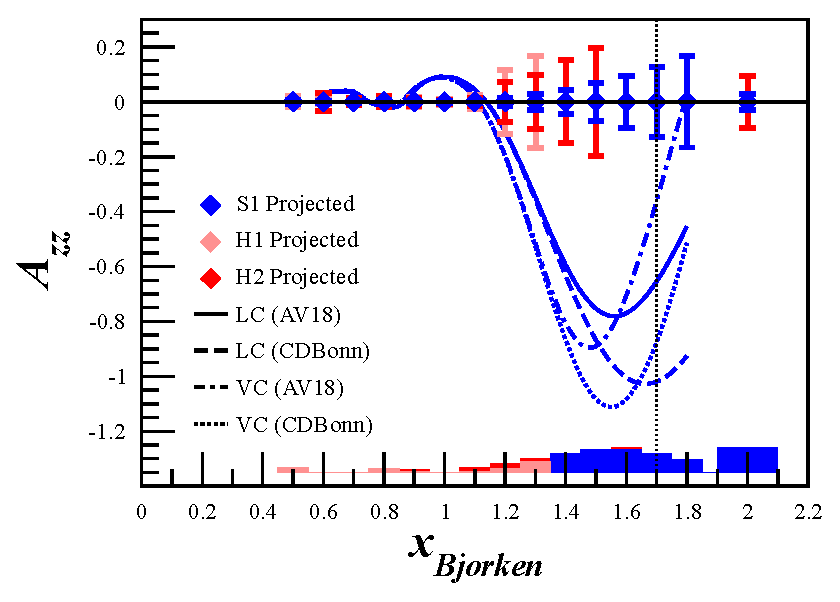
\includegraphics[width=0.49\textwidth]{figs/Azz_S1_H1_H2_vn_lc.eps} 
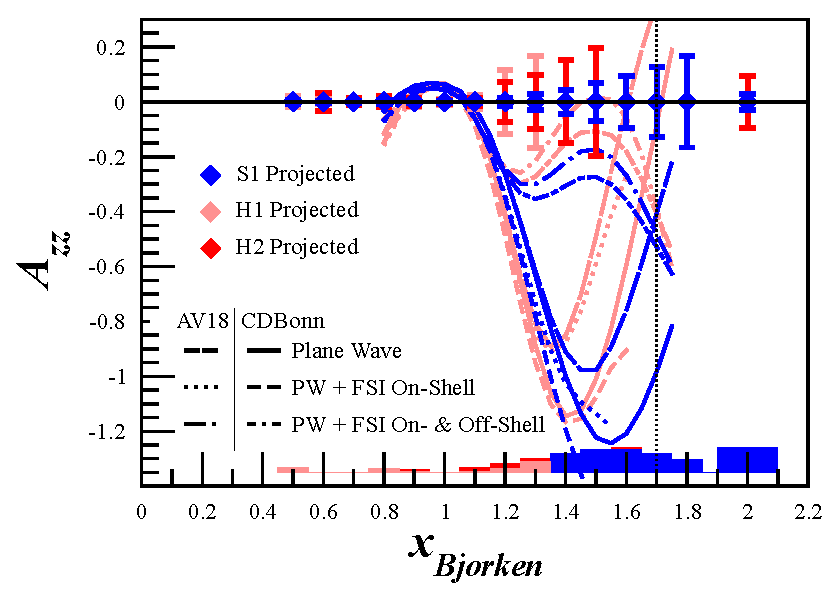
\includegraphics[width=0.49\textwidth]{figs/Azz_S1_H1_H2_fsi.eps} \\
\includegraphics[width=0.49\textwidth]{figs/Azz_S2_H3_S3.eps} 
\caption{\label{PROJ}Projected uncertainties for the tensor asymmetry $A_{zz}$ with \productiondays days of beam time. The band represents the systematic uncertainty. The top row shows the $Q^2>1.0~(\mathrm{GeV}/c)^2$ settings and the bottom row shows the $Q^2<1.0~(\mathrm{GeV}/c)^2$. The upper $x$ limit for H1 (H2) is $x=1.3$ ($x=1.5$). The upper-left plot includes light-cone (LC) and virtual-nucleon (VN) calculations provided by M. Sargsian~\cite{Sargsian:2014fla}, as well as the dependence of each model on various deuteron wave functions (AV18, CDBonn). The dotted line at $x=1.75$ indicates the threshold of $W_{NN}>m_D+100$~MeV where LC and VN calculations begin to not be valid as $A_{zz}$ approaches the elastic peak. The upper-right plot includes virtual-nucleon plane wave and final state interaction (FSI) calculations provided by W. Cosyn~\cite{cosyn-convo}. The bottom row includes a modified Frankfurt and Strikman model~\cite{Frankfurt:1988nt} that estimates the peak shifts in $x$ expected due to the SRC scaling changing with $Q^2$~\cite{Frankfurt:2008zv}.
}
\end{center}
\end{figure}

\begin{figure}
\begin{center}
%\includegraphics[width=0.45\textwidth]{figs/plots0705/b1_proj_newmiller_lin.eps}
%\hspace{0.5cm}
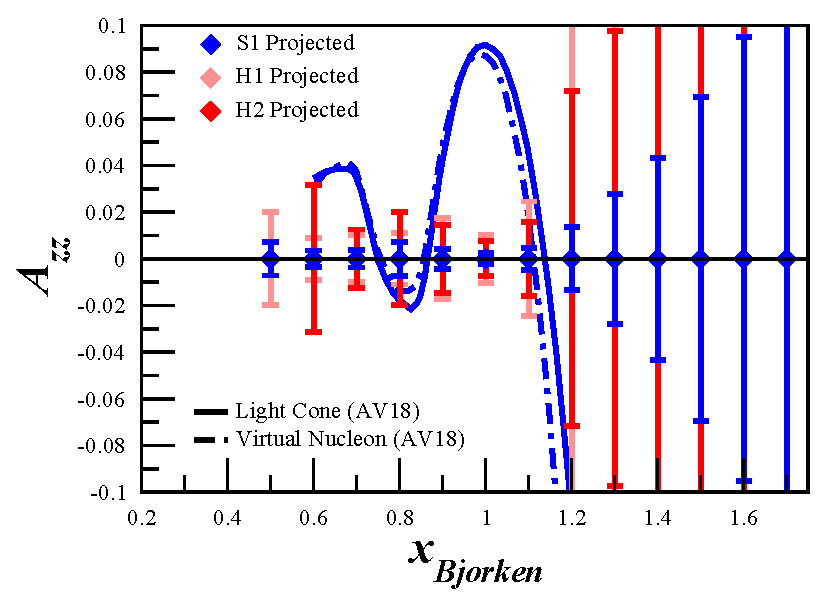
\includegraphics[width=0.49\textwidth]{figs/Azz_S1_H1_H2_zoom.eps} 
\includegraphics[width=0.49\textwidth]{figs/Azz_S2_H3_S3_zoom.eps} 
\caption{\label{PROJ-zoom}Projected uncertainties for the tensor asymmetry $A_{zz}$ with \productiondays days of beam time, same as in Figure~\ref{PROJ}, but zoomed in to $-0.1<A_{zz}<0.1$ to more clearly show the small uncertainties around the quasi-elastic peak.
}
\end{center}
\end{figure}

\begin{table}
\begin{center}
\begin{tabular}{c|c|c|c}
		& $Q^2$    	& $\delta T_{20}^{stat}$	&  $\delta T_{20}^{sys}$ \\
Setting	& (GeV$^2$)	& $\times 10^{-2}$		& $\times 10^{-2}$ \\
\hline\hline
H2 		& 1.8		&  13.2					& 4.7 \\  
S1 		& 1.5		&  3.95					& 4.6 \\
S2 		& 0.7		&  5.36					& 4.6 \\  
H3 		& 0.3		&  4.31					& 9.2 \\  
S3 		& 0.2		&  0.64					& 5.5 \\
  
\hline\hline
\end{tabular}
\caption{\label{RATES-T20}Expected uncertainties for $T_{20}$, assuming a systematic uncertainty of 9.2\%, which could be reduced further by utilizing the S3 measurement as a calibration for the polarized target.}
\end{center}
\end{table}

\begin{figure}
\begin{center}
%\includegraphics[width=0.45\textwidth]{figs/plots0705/b1_proj_newmiller_lin.eps}
%\hspace{0.5cm}
\includegraphics[width=\textwidth]{figs/plot_t20_fit.eps} 
\caption{\label{PROJ-T20}Projected statistical uncertainties for the elastic tensor analyzing power $T_{20}$ with \productiondays days of beam time.
}
\end{center}
\end{figure}

\subsection{Polarized Target}
\label{POLTARGSEC}
This experiment will use the
JLab/UVa dynamically polarized solid {\TARGET}target operated in longitudinal mode.  
%Transverse polarization requires  operation of an upstream chicane to ensure proper transport through the target magnetic field.  
The target is typically operated with a specialized slow raster and beamline instrumentation capable of characterizing the low current 50-100 nA beam.
All of these requirements have been met previously in Hall C.
%, and will be soon implemented also in Hall A for the E08-027/E08-007 run in 2011. 
%
The polarized target (see Fig.~\ref{fig:target}), 
has been successfully used in experiments E143, E155, and E155x at SLAC, and E93-026, E01-006 and E07-003, E08-027 and E08-007 at JLab.
A similar target was used in Hall B for the EG1, EG4, and DVCS experiments. 
%although Hall B does
%not at present have the facilities necessary to operate a transversely polarized target with an electron beam.

The JLab/UVa target underwent significant renovation and improvement~\cite{CKEITH} during the recent g2p run. The magnet was replaced early in the run, and the target then performed consistently.   A new 1 K refrigerator and target insert were designed and constructed by the JLab target group.  The cryogenic pumping system has been overhauled.  In particular, the older Alcatel 2060H rotary vane pumps have been replaced with new Pfeiffer DU065 magnetically coupled rotary vane pumps, and the pump controls are being refurbished. The target motion system has been rebuilt from scratch. %And now, the magnet and vacuum jacket rotate independently of the refrigerator and target insert, which simplifies rotation from parallel to perpendicular magnetic field orientations.

%
\begin{figure}
\centering
\includegraphics[width=5.0in,clip]{figs/targnew.eps} %target_gimp.eps}
\caption{Cross section view of the JLab/UVa polarized target. The proposed experiment will use the modified Hall B magnet, where the backwards-scattering cone is blocked with quench protection circuitry. Figure courtesy of C. Keith.  \label{fig:target}}
\end{figure}


%\begin{figure}
%\centering
%\includegraphics[width=4.5in,clip]{figs/liD.eps}
%\caption{\label{fig:LID} Typical Deuteron thermal equilibrium (TE) and enhanced signals in $^6$LiD.  The left plot shows a typical deuteron TE and the right shows an enhanced deuteron NMR signal.  Note its clean undistorted shape unlike for $^{15}ND_3$.  Also, note the scale difference between the TE and enhanced signals.
%{\it Reproduced from Ref.~\cite{ALTOBIAS}}.}
%\end{figure}

\begin{figure}
\centering
\includegraphics[width=0.5\textwidth]{figs/tensor_pol3.eps}
\caption{{\bf Top}: NMR signal for ND$_3$ with a vector polarization of approximately 50\% from the GEN experiment.  %The average polarization in beam for that experiment was 35\%. 
{\bf Bottom}: Relationship between vector and tensor polarization in equilibrium, and 
neglecting the small quadrupole interaction.  \label{fig:tensorpol}}
\end{figure}

%\begin{figure}
%\centering
%\includegraphics[width=3.0in,clip]{figs/gen.eps} %target_gimp.eps}
%\caption{Performance of the ND$_3$ target during the GEN experiment.  \label{fig:gen}}
%\end{figure}


The target operates on the principle of Dynamic Nuclear Polarization, to
enhance the low temperature (1 K), high magnetic field (5 T) polarization of solid
materials  by microwave pumping.
The polarized target assembly contains several target cells of 3.0 cm length
that can be  selected individually by remote control to be located in the uniform field
region of a superconducting Helmholtz pair. The permeable target cells are
immersed in a  vessel filled with liquid Helium and maintained at 1 K by use of a
high power evaporation refrigerator.
The coils have a 50$^\circ$ conical shaped aperture along the beam axis
which allow for unobstructed forward scattering.
%34$^\circ$ wedge shaped aperture along the vertically oriented midplane.

The target material is exposed to microwaves
to drive the hyperfine transition which  aligns the nucleon spins. 
 The heating of the target by the beam causes a drop of a few percent in
the polarization, and the polarization slowly decreases with time due to radiation
damage. Most of the radiation damage can be repaired by periodically annealing the target,
until the accumulated dose reached is greater than about 
%$ 17\times 10^{15}$ e$^-$/cm$^2$, 
 $0.5\times 10^{17}$~$e^-$/cm$^2$,
at
which time the target material needs to be replaced. 
%The luminosity of the polarized 
%material in the uniform field region is approximately $85\times 10^{33}$ cm$^{-2}$ Hz.

\subsubsection{Polarization Analysis} 
%Eq.~\ref{TENSORVECTOR} allows calculation of a target's tensor polarization once the vector polarization has been determined.  
The three Zeeman sublevels of the deuteron system ($m=-1,0,1$) are
shifted unevenly due to the quadrupole interaction~\cite{Meyer:1985dta}. This shift
depends on the angle between the magnetic field and the electrical field gradient, and gives rise to two separate transition
energies. Hence, the unique double peaked response displayed in Fig.~\ref{fig:tensorpol}.
When the system is at thermal equilibrium with the solid lattice, the deuteron polarization is known from:
\begin{eqnarray}
\label{VECT}
P_z = \frac{4+\tanh\frac{\mu B}{2 k T}} {3+\tanh^2\frac{\mu B}{2 k T}    }
\end{eqnarray}
where $\mu$ is the magnetic moment, and $k$ is Boltzmann's constant.  The vector polarization can be determined by comparing
the enhanced signal with that of the TE signal (which has known polarization).  This polarimetry method is typically reliable to about 3.9\% relative.

Similarly, the tensor polarization is given by: 
\begin{eqnarray}
\label{TENS}
P_{zz} = \frac{4+\tanh^2\frac{\mu B}{2 k T}} {3+\tanh^2\frac{\mu B}{2 k T}    }
\end{eqnarray}

From Eqs.~\ref{VECT} and~\ref{TENS}, we find:
\begin{eqnarray*}
\label{PZZEQN}
P_{zz}= 2 - \sqrt{4-3 P_z^2}
\end{eqnarray*}


In addition to the TE method, polarizations can be determined by analyzing NMR lineshapes as described in~\cite{Dulya:1997qc} with a typical  7\% relative uncertainty.  At high polarizations, the
intensities of the two transitions differ, and the NMR signal shows an asymmetry R in the
value of the two peaks, as shown in Fig.~\ref{fig:tensorpol}.  The vector polarization is then given by:
\begin{eqnarray}
\label{RVECT}
P_{z} = \frac{R^2-1}{R^2+R+1}
\end{eqnarray}
and the tensor polarization is given by:
\begin{eqnarray}
\label{TVECT}P_{zz} = \frac{R^2-2 R +1}{R^2+R+1}
\end{eqnarray}
This measuring technique can be used as a compliment to the TE method resulting in reduced uncertainty in polarization.


\subsubsection{Tensor Polarization Enhancement}
It is possible to enhance tensor polarization using RF irradiation on the oriented deuterium nuclei to manipulate the alignment.
Applying a saturating RF field on the pedestal of the smaller transition equalizes the substate $m=+1$ and $m=0$ populations
over 2/3 of the NMR signal.  This equalization over the range of a single pedestal leads to enhancement in tensor polarization with only a small loss
to the overall area ($\sim 2\%$).  Very recent studies at UVA using deuterated butanol have indicated that the tensor polarization can be increased by using a modified hole burning technique. The result will be investigated in the near future, and the method applied to ND$_3$.
% in a tensor polarization of more then25\% as shown in Fig.~\ref{fig:study}.  A similar result is expected for ND$_3$.  
The studies also indicate that microwaves used during DNP does not
interfere with the saturation from the RF irradiation when sufficient power is used.  This implies that RF over the pedestal can be done the same time DNP is performed to enhance the area while taking beam in an experiment.  Research and development is ongoing to study various
techniques to optimize tensor enhancement for nuclear experiments targets.
\begin{figure}
\centering
\includegraphics[width=3.0in,clip]{figs/study.eps}
\caption{The deuterium magnetic resonance line shape showing the recent achievement of 
%more than 25\%
high tensor polarization of deuterated butanol after RF saturation of a pedestal at the UVA polarized target lab accomplished during their April 2014 cool-down.}  
\label{fig:study}
\end{figure}

\subsubsection{Depolarizing the Target}
%The NMR will be used on both to probe polarization.  
To move from polarized to unpolarized measurements, the target
polarization will be annihilated using destructive NMR loop field changes and destructive DNP microwave pumping.
%It is also possible to remove LHe in the nose of the target to remove the polarization by heating.
During unpolarized data taking the incident electron beam heating is enough to remove the thermal equilibrium polarization.

We are able to verify that the target is in the unpolarized state via NMR measurements.  The target material will be
kept at 1 K for polarized and unpolarized data collection, and the target field
will be held constant for both states as well.  These
consistencies are used to minimize the systematic differences in the
polarized and unpolarized data collection.  To minimize systematic effects over
time, the polarization condition will be switched twice in a 72 hour period, as shown in Fig.~\ref{fig:polcycle}. 
This will be sufficient to account for drift in integrated charge accumulation.

\begin{figure}
\centering
\includegraphics[width=0.75\textwidth,clip]{figs/pol_cycle.eps}
\caption{A visual demonstration of how the polarization cycle will happen over a 72 hour period to reduce time-dependent systematic effects. For the two lower $Q^2$ measurements, the cycle will happen over a 18 hour period.}  
\label{fig:polcycle}
\end{figure}

%(I think we should move this discussion to another section dealing with target
%physics and the overhead time accounting. Also,  I would favor dumping the LHe, and refilling the
%nose.)}


\subsubsection{Dilution Factor}
\label{dil}
To derive the dilution factor, we first start with the ratio of 
polarized to unpolarized counts.
%equation used to obtain the observable in terms of each measured cross section.
%\begin{equation}
%\frac{A_{zz}P_{zz}}{2}=\left(\frac{\sigma^1-\sigma}{\sigma}\right).
%\end{equation}
In each case, the number of counts that are actually measured,  neglecting 
the small contributions of the thin aluminium cup window materials, NMR coils, etc.,
are
\begin{equation}
N_1=Q_1\varepsilon_1 {\cal A}_1 l_1[(\sigma_N+3\sigma_1)p_f+\sigma_{He}(1-p_f)],
\end{equation}
and
\begin{equation}
N=Q\varepsilon {\cal A}l[(\sigma_N+3\sigma)p_f+\sigma_{He}(1-p_f)].
\end{equation}
where $Q$ represents accumulated charge, $\varepsilon$ is the dectector 
efficiency, ${\cal A}$ the cup acceptance, and $l$ the cup length.  

For
this calculation we assume similar charge accumulation such that $Q\simeq Q_1$, 
and that the efficiencies stay constant, in which case all factors drop out of 
the ratio leading to
\begin{eqnarray}
\nonumber \frac{N_1}{N}& = &\frac{{(\sigma_N+3\sigma_1)p_f+\sigma_{He}(1-p_f)}
}{(\sigma_N+3\sigma)p_f+\sigma_{He}(1-p_f)}\\
\nonumber & = & \frac{{(\sigma_N+3\sigma(1+A_{zz}P_{zz}/2))p_f+\sigma_{He}(1-p_
f)}}{(\sigma_N+3\sigma)p_f+\sigma_{He}(1-p_f)}\\
\nonumber & = & \frac{{[(\sigma_N+3\sigma)p_f+\sigma_{He}(1-p_
f)]+3\sigma A_{zz}P_{zz}/2}}{(\sigma_N+3\sigma)p_f+\sigma_{He}(1-p_f)}\\
\nonumber & = & 1 + \frac{3\sigma 
A_{zz}P_{zz}/2}{(\sigma_N+3\sigma)p_f+\sigma_{He}(1-p_f)}\\
& = & 1 + \frac{1}{2} f A_{zz}P_{zz}, 
\end{eqnarray}
where $\sigma_1 = \sigma(1+A_{zz}P_{zz}/2)$ has ben substituted, per 
Eq.~\ref{eq:one}, with $P_B =0$. It can be seen that the above result 
corresponds to Eq.~\ref{3}.

\subsection{Overhead}

Table~\ref{OVERHEAD} summarizes the expected overhead, which sums to \overheaddays days.
%In order to calibrate the target polarimetry, elastic scattering measurements will be performed at %an
%incident energy of 2.2 GeV.
The dominant overhead comes from switching from the polarized to unpolarized state and vice versa, and target anneals.  The target will need to be annealed about every other day, and the material replaced once a week.
Measurements of the dilution from the unpolarized materials contained in the target, and of the packing fraction due to the granular composition of the target material will be performed with a carbon target.

%Configuration changes include rotation of the magnetic field of the target from parallel to perpendicular and vice versa.

\begin{table}
\begin{center}
  \begin{tabular}{lrrr} \hline\hline
 Overhead & Number&Time Per (hr)&(hr)\\
\hline
Polarization/depolarization & 35&       2.0&     70.0\\
Target anneal             &   13&       4.0&     52.0\\
Target T.E. measurement   &    5&       4.0&     20.0\\
%Beamline survey          &    2&       8.0&     16.0\\
Target material change    &    4&       4.0&     16.0\\
Packing Fraction/Dilution runs &    18&       1.0&      18.0\\
\hline
%Pass change              &    0&       4.0&       0.0\\
BCM calibration           &    8&       2.0&      16.0\\
Optics                    &    3&       4.0&      12.0\\
Linac change              &    1&       8.0&      8.0\\
Momentum/angle change     &    3&       2.0&       6.0\\
%Arc Energy Meas.          &    3&       2.0&       6.0\\
\hline
                          &     &          &        \overheaddays days  \\
\hline
 \end{tabular}
 \end{center}
  \caption{\label{OVERHEAD} Major contributions to the overhead.}
\end{table}


\section{PAC42 Comments and Concerns}

In this section we summarize the comments and concerns that were raised by the PAC42 committees on letter of intent LOI12-14-002.

\subsection{Theory Advisory Committee}

\begin{quote}
``This Letter of Intent describes a measurement of the tensor-polarized asymmetry $A_{zz}$ in electron scattering on polarized deuterium in the quasi-elastic region, at values of $x = 0.8 - 1.75$ ($x$ is the equivalent Bjorken variable at the nucleon level) and $Q^2 = 1 − 2 \mathrm{~GeV} ^2$. The aim is to determine with this observable the $S/D$ wave ratio in the deuteron wave function at large relative momenta $k > 300$~MeV, which is important for understanding the $NN$ interaction at short distances and the properties of the dominant $pn$ short-range correlations in heavier nuclei. The same tensor-polarized asymmetry was/will be measured in elastic scattering (deuteron form factor) and deep-inelastic scattering (structure function $b_1$); the proposed measurement in quasi-elastic scattering would fill the gap and study this observable in the region where it is most directly related to the short-range $NN$ interaction. The tensor asymmetry at large recoil momenta also serves as a sensitive test of ``relativistic effects" in the treatment of deuteron structure, which are an important aspect of the overall theoretical framework and the object of ongoing studies. A unique feature of the measurement proposed here is that it selects small-size configurations in the deuteron both through the tensor asymmetry ($D$-state) and the choice of kinematics ($x > 1$), amplifying the overall effect. The use of $x > 1$ for selecting small-size $NN$ configurations has been demonstrated in previous studies of deep-inelastic structure. 

The measurement proposed here arises from a well-developed context, presents a clear objective, and enjoys strong theory support. It would further explore the nature of short-range $pn$ correlations in nuclei, the discovery of which has been one of the most important results of the JLab 6 GeV nuclear program. Development of a full proposal should be encouraged."
\end{quote}

\subsection{Technical Advisory Committee}

\begin{quote}
``This experiment utilizes the same apparatus and techniques as the conditionally approved b1 experiment C13-12-011. The comments in the TAC report for that experiment also apply to this experiment.

The requirement to understand and mitigate time-dependent systematic effects may be less as the asymmetry $A_{zz}$, at least for $x>1$, is expected to be larger than for b1. 
However, measuring with $\delta A_{zz} < 0.10$ still requires a systematic control of the raw asymmetry to better than 1\%. 
This is still challenging with a target polarization that is cycled on and off about once a day.
Furthermore, at $x>1$, short range structure enhances inclusive cross sections in nuclei relative to deuterium. This will reduce the dilution factor for $x>1$ measurements, reducing the raw asymmetries to levels where understanding and controlling systematic errors will still be important."
\end{quote}

\subsection{Program Advisory Committee}
\begin{quote}
``\textbf{Measurement and Feasibility:} Electron scattering off tensor-polarized deuterium would be measured in the quasi-elastic
region using the Hall C HMS and SHMS spectrometers. This proposal would use the same setup as the C1-approved
experiment E12-13-011, which is to measure the deuteron tensor structure function b1. The C1-approval is subject to
demonstration that 35\% tensor polarization is possible. The expected asymmetry is larger in the case of this measurement,
but we anticipate that a similar requirement would apply. It is anticipated that a full proposal would be for 39 days, which
would include 30 days for three different $Q^2$ values and 9.1 additional days of overhead.

\textbf{Issues:} A significant amount of beam time will be required for this measurement. A full proposal will need a detail
discussion of expected systematic and statistical errors similar to what is in the letter that carefully justifies the requested
time. The proposal should also demonstrate what sensitivity they will have to NN interaction models, such as the 6-quark
model, final state interaction models, and NN interaction models, mentioned in the proposal. It will also be important to
discuss how the results will distinguish between effects from the NN-interaction, the treatment of these interactions at
high virtuality, and the intrinsic deuteron wave function.

\textbf{Recommendation:} Proceed to proposal addressing the issues noted above."
\end{quote}

\subsection{Response to PAC42 Concerns}
The tensor polarization of 30\% used in the rates for this proposal is the same as condition on the E12-13-011 proposal, which was incorrectly mentioned as 35\%. To ensure that the target polarization is not significantly affected by the electron beam, we've reduced our estimated current from 90~nA in the LOI to \CURRENT~nA, which is the conservative standard for a DNP target. We have expanded upon our estimated statistical and systematic uncertainties in Section \ref{uncertainties} and in a recent technical note\need, where we stress that a measurement of $A_{zz}$ in the quasi-elastic and $x>1$ region is ideal for understanding time-dependent systematic effects without significantly affecting the measurement, as it is an order of magnitude less sensitive to drift effects than $b_1$. Furthermore, we will be measuring $T_{20}$ at low $Q^2$ where the observable is well understood both experimentally and theoretically, which can be used as a calibration to reduce our leading systematics from understanding the target polarization. There has also been a dedicated effort made in understanding the tensor-enhanced polarization state by the UVA group over the past few years. Through studying tensor polarization and NMR line-shape analysis through multiple cool-downs, the UVA group is confident that the uncertainty in polarization can be kept to $<6\%$~\cite{keller2, keller3}. However, even a very conservative estimate of $10\%$ would make for a compelling measurement.
%However, for the uncertainty calculations in this proposal we retain a conservative estimate of 12\%.


Since PAC42, we have engaged a number of theorists who have provided models not only between light cone and virtual nucleon models, but also using different $NN$ interaction potentials~\cite{Sargsian:2014fla} and final state interactions~\cite{cosyn-convo}. Deviations based on $NN$ potentials only become apparent at large $x>1.3$, so that the low $x<1.3$ region can be used to discriminate between light cone and virtual nucleon calculations. Furthermore, $A_{zz}$ calculations are currently being systematically studied at low $Q^2$ by W. Van Orden and are expected to be completed within a year~\cite{vanorden-convo}. Although not completed at the time of this proposal, G. Miller is still engaged in providing calculations of 6 quark effects in the elastic region~\cite{miller-convo}. Additionally, the proposed $A_{zz}$ measurements are also ideal for making simultaneous high-precision measurements of $T_{20}$ to test existing calculations up to large $Q^2$, as discussed in Section~\ref{t20_exp}, including in the region where Hall C and MIT-Bates data show a discrepancy, which requires only four more days of beam time than initially proposed in the LOI. Along with the ground-breaking measurements of $A_{zz}$ in the $x>1$ region, we will also be measuring $T_{20}$ in the largest $Q^2$ range ever taken in a single experiment.







\section{Summary}


We have investigated the possibility of making high precision measurements of the quasi-elastic tensor asymmetry $A_{zz}$.  By covering the kinematic range from the QE peak ($x\approx 1$) up to elastic scattering ($x=2$), we expect that this data will provide valuable new insights about the high momentum components of the deuteron wavefunction. We have been actively working with several theorists who have provided state-of-the-art calculations of light cone, virtual nucleon, and final state interactions. Additional calculations are being performed that include six-quark models, and low $Q^2$ sensitivity to NN potentials.  It is important to note that this is the same kinematic region that has been shown to be correlated with the EMC effect via the $x>1$ A/D ($e,e'$) results. 

Additionally, our measurement of $A_{zz}$ allows for a simultaneous measurement of the tensor analyzing power $T_{20}$ without any further beam time or equipment by making a kinematic cut on the elastic peak. The lowest $Q^2$ measurement will fall on the most experimentally probed and theoretically understood region, making it ideal for ensuring that the tensor polarized target is operating correctly and to help reduce target systematic uncertainty, the leading systematic in this experiment. At medium $Q^2$, our measurement will fall in the same region where there is currently a discrepancy between Hall C and Bates results. Our final point will lie at the highest $Q^2$ value ever measured for $T_{20}$, and will provide a crucial test of ensuring our understanding of $T_{20}$. These measurements of $T_{20}$ will also cover the largest range in $Q^2$ measured by a single experiment.


We have found that with \productiondays days of beam and an additional \overheaddays days of overhead, $A_{zz}$ can be measured with high precision at $Q^2=0.2$, 0.3, 0.7, 1.5, 1.8 and $2.9~(\mathrm{GeV}/c)^2$ and $T_{20}$ at $Q^2=0.2$, 0.3, 0.7, 1.5, and $1.8~(\mathrm{GeV}/c)^2$ in Hall C using identical equipment as the upcoming $b_1$ measurement while being orders of magnitude less sensitive to systematic uncertainties. In addition, this data will fill a gap in measurements of $A_{zz}$ between the $T_{20}\propto A_{zz}$ elastic measurements and the $b_1\propto \frac{A_{zz}}{F_1^d}$ deep-inelastic measurements. 

% -----------------------------------------------------



% \section{Summary}

\clearpage
\appendix
%\section{Rates and Kinematics}
%\begin{figure}
%\begin{center}
%\includegraphics[width=1.0\textwidth,angle=00]{newfigs/ellie/b1_rates_hms_shms.eps}
%\caption{\label{PROJDETAIL}
%{\bf Top Left: }
%Projected precision of the tensor structure function $b_1$  with \production_days days of beam time.
%{\bf Right:}
%Corresponding projected precision of the tensor asymmetry $A_{zz}$.
%Data at different $Q^2$ are combined with an x-binning that varies slightly per point, but is approximately $\pm0.05$.
%%The black band
%%represents the systematic uncertainty.
%Also shown are the HERMES data~\cite{Airapetian:2005cb}, and the calculations from Kumano~\cite{Kumano:2010vz}, Miller~\cite{Miller:1989nc,Miller_tmp}, and Sargsian~\cite{MISAK}.
%}
%\end{center}
%\end{figure}

%\section{Statistical error calculations of $A_{zz}$}
%\input{input/Azz_error.tex}
%\input{input/b1_error.tex}
%%\section{Statistical Uncertainty Calculation}
\label{stat}
To investigate the statistical uncertainty we start with the equation for $A_{zz}$ using
measured counts for polarized data $N_1$ and unpolarized data $N$, 
\begin{equation}
A_{zz}=\frac{2}{fP_{zz}}\left(\frac{N_1-N}{N}\right).
\end{equation}
The absolute error with respect to counts in then,
\begin{equation}
\delta A_{zz}=\frac{2}{fP_{zz}}\sqrt{\left(\frac{\delta N_1}{N}\right)^2+\left(\frac{N_1\delta N}{N^2}\right)^2}.
\end{equation}
To approximate, assume $N_1\simeq N$, so that twice $N$ is required to obtain the total number of count
$N_T$ for the experiment leading to,
\begin{equation}
\delta A_{zz}=\frac{4}{fP_{zz}}\frac{1}{\sqrt{N_T}}.
\end{equation}



%  Go to fullpage mode

\topmargin 0pt
\advance \topmargin by -\headheight
\advance \topmargin by -\headsep

\textheight 8.9in

\oddsidemargin 0pt
\evensidemargin \oddsidemargin
\marginparwidth 0.5in

\textwidth 6.5in
\clearpage
%\begin{thebibliography}{99}
%\input{input/bib.tex}
%\end{thebibliography}

\bibliography{input/bibliography}
\end{document}
